% Векторизация.
\newpage
\section*{Глава 5. Векторизация вычислений} % выключить номер главы
\addcontentsline{toc}{section}{Глава 5. Векторизация вычислений} % но добавить ее в оглавление
\addtocounter{section}{1}                                                    % а теперь и счетчик продвинуть
\setcounter{subsection}{0}
\setcounter{figure}{0}
\setcounter{equation}{0}
\setcounter{table}{0}
\setcounter{theorem}{0}
\setcounter{lemma}{0}
\setcounter{definition}{0}

% Описательная часть про векторизацию.
Векторизация вычислений это низкоуровневая оптимизация, применение которой способно кратно повысить производительность наиболее часто исполняемых участков программного кода и сократить энергопотребление \cite{Cebrian2019VecScal}.
Использование векторных инструкций позволяет применять одинаковые операции сразу к нескольким наборам входных данных, упакованных в векторные регистры.
Векторные инструкции представлены во многих современных микропроцессорным архитектурах, но в наибольшей степени они развиты в архитектуре x86.

% x86
Архитектура x86 представлена богатым набором векторных инструкций, которые добавлялись постепенно по мере развития \cite{IntelSDM2025}.
Первый набор инструкций MMX\label{abbr:mmx-1} был предназначен для обработки аудио и видеоданных и содержал операции по работе с целыми числами, упакованными в 64-битные регистры.
В дальнейшем в архитектуру были добавлены несколько наборов SSE\label{abbr:sse-1} и AVX\label{abbr:avx-2} инструкций, и на сегодняшний день последним расширением является AVX-512 с возможностью выборочной обработки элементов векторов, о котором в основном и будет идти речь в этой главе.

Упомянем кратко другие микропроцессорные архитектуры, в которых можно встретить поддержку векторных вычислений.

% ARM
В архитектуре ARM\label{abbr:arm-1} векторные инструкции поддержаны в 128-битном SIMD\label{abbr:simd-1} расширении Neon, и они являются по сути аналогом SSE инструкций в x86 \cite{Zhuykov2012VecARM,Marquez2020VecARM}.
Инструкции Neon поддерживают работу с целыми элементами данных размера от 8 до 64 битов, а также с вещественными значениями размера 16, 32 и 64 бита.
Инструкции Neon не поддерживают выборочную обработку элементов данных векторов, однако в наборе предусмотрены широкие возможности комбинирования данных путем выполнения операций сдвига и перестановки элементов внутри вектора.
Современное расширение SVE\label{abbr:sve-1} \cite{Stephens2017VecARM} позволяет оперировать терминами векторных вычислений без привязки к конкретной длине вектора (при условии кратности 128), которая определяется аппаратной реализацией.
В частности, в микропроцессоре Fujitsu A64FX используется набор SVE инструкций с реализаций длины вектора 512-бит \cite{Okazaki2020A64FX}.

% Power
Для поддержки векторных и матричных вычислений в архитектуре Power предусмотрено векторное расширение VMX\label{abbr:vmx-1} \cite{Gschwind2016VecPower,Eisen2007VecPower}.
Расширение поддерживает векторные регистры, состоящие из целых значений размера до 32 битов, либо вещественные значения одинарной точности.
В расширение входят арифметические и логические операции, операции доступа в память, однако выборочная обработка элементов векторов не поддержана.

% Эльбрус
В архитектуре <<Эльбрус>> присутствует поддержка векторных операций для коротких векторов размера 64 бита, что позволяет паралльно выполнять арифметические операции над элементами векторов \cite{Ishin2011VecElbrus}.
Так как выборочная обработка элементов векторов в этом наборе инструкций также отсутствует, то для векторизации управления в цикле используются логические операции обнуления ненужных частей соответствующих векторных регистров с последующим их слиянием \cite{Volkonsky2012VecElbrus}.

% Китайские.
Можно отметить современные китайские микропроцессорные архитектуры, также поддерживающие векторизацию.
Так, в оригинальной архитектуре LoongArch, на базе которой создан микропроцессор Loongson 3A6000, поддержаны векторные инструкции, работающие с упакованными векторами размера 128 и 256 бит \cite{Bai2024VecLoongarch}.
А в архитектуре Sunway \cite{Sun2023VecSunway}, на базе которой собрана одна из мощнейших линеек китайских суперкомпьютеров, в систему команд включены инструкции для работы с 512-битными векторами.

Для оценки качества векторизации программного кода в этой главе будем использовать следующие понятия.

\begin{definition}
Шириной векторизации назовем величину $w = \frac{v}{t}$, где $v$ -- размер векторного регистра, $t$ -- размер типа расчетных данных.
\end{definition}

То есть, например, при выполнении расчетов на вещественных данных одинарной точности (float, размер 32 бита) ширина векторизации при использовании AVX-512\label{abbr:avx-3} (размер векторного регистра 512 битов) равна 16.

\begin{definition}
Ускорением программного кода от векторизации будем называть величину $s_{vec} = \frac{T}{T_v}$, где $T$ -- время выполнения невекторизованной (скалярной) версии кода, $T_v$ -- время выполнения векторизованной версии кода.
\end{definition}

\begin{definition}
Эффективностью векторизации будем называть величину $e_{vec} = \frac{s_{vec}}{w}$.
\end{definition}

Показатель эффективности векторизации является удобной мерой сравнения векторизованного кода.
При этом следует отметить, что $e_{vec}$ вполне может превышать единицу при использовании, например, большого количества векторных FMA\label{abbr:fma-1} операций.
Однако, в большинстве случаев этот показатель меньше единицы.

\begin{definition}
Логическим ускорением программного кода от векторизации будем называть величину $s_{vec}^{*} = \frac{L}{L_v}$, где $L$ -- количество выполненных инструкций в скалярном коде, $L_v$ -- количество выполненных аналогичных им инструкций в векторном коде.
\end{definition}

\begin{definition}
Логической эффективностью векторизации будем называть величину $e_{vec}^{*} = \frac{s_{vec}^{*}}{w}$.
\end{definition}

%---------------------------------------------------------------------------------------------------
% 5.1 - AVX-512

\subsection{Векторные инструкции AVX-512}\label{abbr:avx-4}

На сегодняшний день наиболее продвинутым набором векторных инструкций является AVX-512, поддержку которого можно встретить в микропроцессорах Intel и AMD\label{abbr:amd-1}.
Инструкции AVX-512 работают с векторными регистрами zmm размера 512 бит, каждый из которых вмещает в себя 8 элементов в формате вещественных чисел двойной точности, что с учетом комбинированных операций приводит к возможности выполнения 16 операций сложения и умножения двойной точности за одну векторную команду.
Из этого следует, что на микропроцессорах с поддержкой AVX-512 без использования векторизации даже теоретически невозможно добиться производительности более 6,25\% от пиковой производительности.
Особенности векторных инструкций AVX-512 позволяют применять их для векторизации достаточно сложного программного контекста, однако оптимизирующий компилятор не всегда успешно справляется с этой задачей.
Для обеспечения программисту возможности прямого использования векторных инструкций существует набор функций-интринсиков \cite{IntelIntrinsicsGuide}, которые в дальнейшем заменяются компилятором на конкретные векторные инструкции или последовательности инструкций.
Использование интринсиков значительно упрощает разработку векторизованного кода и позволяет вести разработку в терминах функций, применяемых к векторным данным.

Можно считать, что впервые набор векторных инструкций AVX-512 был поддержан в 2016 году в микропроцессорах Intel Xeon Phi KNL\label{abbr:knl-5} \cite{Jeffers2016KNL}, так как более раннее поколение Intel Xeon Phi Knights Corner (KNC)\label{abbr:knc-1} представляет собой ускоритель, и векторный код для него не является x86 совместимым.
С этого момента вопросы векторизации приложений активно обсуждаются в научном сообществе.

\subsubsection{Обзор применения инструкций AVX-512}

Отметим наиболее заметные актуальные работы, в которых описаны существенные результаты по ускорению программных кодов, полученные с помощью векторизации.

В работе \cite{Kulikov2019VecAstro} путем векторизации безусловных операций было продемонстрировано повышение производительности газодинамического решателя на 200\% при исполнении на микропроцессорах Intel Xeon Phi KNL и Intel Xeon Scalable.
В работе \cite{Glinting2019VecSwim} описывается сравнение реализации римановских решателей в применении к теории мелкой воды, одним из результатов работы является ускорение решателя с помощью инструкций AVX-512 в 16,7 раз при работе с вещественными числами одинарной точности.
В исследовании \cite{Yildirim2021VecCFD} было достигнуто ускорение в 3,27 газодинамического решателя ADflow, работающего на структурированных расчетных сетках.
Ускорение достигнуто путем декомпозиции сетки на вычислительные блоки, которые могут быть эффективно обработаны с точки зрения использования кэш-памяти и применения векторных инструкций AVX-512.
В работе \cite{Rucci2020VecNBody} рассмотрена реализация расчета гравитационного взаимодействия между N телами, из результатов видно, что использование набора инструкций AVX-512 позволило ускорить работу приложения в 2 и более раз.
В работе \cite{Rucci2019VecSW} описано успешное применение векторных инструкций в задаче поиска сходных участков в белковых последовательностях.
Работы \cite{Choi2023VecKorean,Cheng2021VecCSIDH} посвящены ускорению алгоритмов, связанных с шифрованием.

В качестве практического руководства по созданию векторизованного программного кода с помощью функций-интринсиков для языка программирования C++ и с помощью языка ассемблера для широкого спектра практических задач, включая задачи линейной алгебры, обработки изображений, реализацию сверток и другие, можно рассматривать работу \cite{Kusswurm2022VecCpp}.

Среди научно-исследовательских статей в различных областях применения можно отметить \cite{Blacher2022VecQuick}, посвященную разработке векторизованной версии быстрой сортировки (vqsort) с помощью наборов векторных инструкций AVX2 и AVX-512, превышающей по эффективности реализацию из стандартной библиотеки (qsort) более чем в 10 раз.
В работе \cite{Long2022VecSPD} рассматриваются реализация бессеточного метода решения задачи газовой динамики и векторизация этого метода. 
Использование векторных инструкций AVX-512 позволило ускорить исходный код в 6,3 раза.
В статье \cite{PonteFernandez2022VecInteractions} описано успешное применение векторизации для алгоритма анализа генетических вариаций.
Использование векторных инструкций AVX-512 позволило добиться ускорения расчетов от 7 до 12 раз по сравнению с оригинальным алгоритмом (алгоритм базируется на обработке данных формата Byte, что объясняет такое серьезное ускорение).
В работе \cite{Quisland2023VecSeries} рассматривается прямое применение инструкций AVX-512 для задачи обработки временных рядов, что привело к ускорению результирующего кода в 4 раза по сравнению с автоматической векторизацией, выполняемой оптимизирующим компилятором. 
Статья \cite{Buhrow2022VecMult} посвящена оптимизации алгоритмов шифрования с открытым ключом, в частности, рассматривается оптимизация блочного варианта умножения Монтгомери.
Было достигнуто ускорение основных операций от 1,5 до 1,9 раза.
В статье \cite{Choi2022VecPIPO} показана реализация алгоритма блочного шифрования на различных архитектурах, включая GPU\label{abbr:gpu-1} и CPU\label{abbr:cpu-1}.
В частности, в рамках этой работы алгоритм блочного шифрования был реализован с помощью инструкций AVX-512, что позволило ускорить его в 9,5 раза по сравнению с оригиналом.
В статье \cite{Cheng2022VecSIKE} рассматривается применение векторных инструкций для оптимизации математических операций, используемых в протоколе обмена ключами с применением суперсингулярных изогений (SIKE)\label{abbr:sike-1}.
В результате выполненных усовершенствований зафиксировано ускорение отдельных операций в диапазоне от 1,5 до 3,5 раза.
В работе \cite{Sansone2023VecFourier} описано использование инструкций AVX-512 для оптимизации быстрого преобразования Фурье.
С помощью функций-интринсиков для векторных инструкций было достигнуто ускорение примерно в полтора раза по сравнению с оригинальной версией.
Работа \cite{Edamatsu2023VecDiv} посвящена применению подмножества инструкций Integer Fused Multiply-Add (AVX-512 IFMA)\label{abbr:ifma-1} для повышения эффективности реализации деления больших целых чисел.
В результате оптимизации было достигнуто ускорение требуемого функционала на 25–35\%.
В работе \cite{Medakin2021VecPP} продемонстрирован практический подход к векторизации расчета попарного взаимодействия множества частиц.
Использование инструкций AVX-512 в явном виде привело к ускорению исполнения программы в 3,3 раза.
В статье \cite{Tayeb2023VecAuto} предлагается подход к развитию средств автоматической векторизации расчетных циклов, основанный на анализе и эквивалентных преобразованиях графа зависимостей между операциями, расположенными в теле цикла.
Этот подход позволяет переупорядочить операции внутри цикла, снизив их количество и укоротив критический путь исполнения \cite{Laukemann2019VecAuto}, и сгруппировать для объединения в векторные инструкции.

\subsubsection{Особенности инструкций AVX-512}

Множество инструкций AVX-512\label{abbr:avx-5} состоит из нескольких подмножеств, их перечень расширяется с появлением новых поколений микропроцессоров (при этом в различных поколениях микропроцессоров поддержаны разные наборы подмножеств инструкций AVX-512) \cite{IntelSDM2025}.
Приведем краткое описание этих поднаборов.

AVX-512 F (Foundation) -- основной набор, который содержит в себе базовые операции для работы с векторными данными, включая арифметику, операции конвертации, сравнения, операции перестановки элементов векторов и другие.

Набор AVX-512 VL\label{abbr:vl-1} (Vector Length) позволяет расширить многие векторные инструкции для работы со 128-битными XMM регистрами и 256-битными YMM регистрами на длину вектора 512.

Набор AVX-512 BW\label{abbr:bw-1} (Byte and Word) расширяет инструкции для работы с элементами векторов размера 8 и 16 бит, а AVX-512 DQ\label{abbr:dq-1} (Doubleword and Quadword) добавляет новые инструкции, работающие с элементами размера 32 и 64 бита.

Набор AVX-512 CD\label{abbr:cd-1} (Conflict Detection) содержит операцию для нахождения пар совпадающих целых значений в двух векторах (VPCONFLICTD/Q), а также операции записи маски в элементы вектора и подсчета количества ведущих нулей в элементах вектора.
Операции подсчета количества единиц в элементах векторов определены в наборах AVX-512 BITALG\label{abbr:bitalg-1} (Bit Algorithms) и AVX-512 VPOPCNTDQ (Vector population count).

AVX-512 ER\label{abbr:er-1} (Exponential and Reciprocal) включает в себя инструкции для вычисления значений $2^x$, $1/x$, $1/{x^2}$.

AVX-512 PF\label{abbr:pf-1} (PreFetch) содержит операции предварительной подкачки данных для VGATHERDPS/VSCATTERDPD, что позволяет уменьшить вероятность промаха в кэш при дальнейших обращениях в память.

Наборы AVX-512 VBMI\label{abbr:vbmi-1} (Vector Byte Manipulation Instructions) и AVX-512 VBMI2 добавляют новые операции, работающие с 8-битными данными, такие как перестановка элементов, чтение из памяти и запись в память, конкатенация со сдвигом.

AVX-512 IFMA\label{abbr:ifma-2} (Integer Fused Multiply Add) содержит комбинированные операции над целыми числами, которые используются для реализации работы с большими числами или для шифрования \cite{Edamatsu2023VecDiv}.

Набор AVX-512 FP16\label{abbr:fp-1} включает в себя арифметические операции и операции конвертации для работы с вещественными числами половинной точности, а набор AVX-512 BF16\label{abbr:bf-1} добавляет инструкции для работы с форматом brain float 16 \cite{Kalamkar2019VecBF16}.

AVX-512 VNNI\label{abbr:vnni-1} (Vector Neural Network Instructions) и AVX-512 4VNNIW\label{abbr:vnniw-1} содержат операции поэлементного перемножения пар целых чисел с последующим их сложением.
Операции выполняются над 8-битными и 16-битными данными и используются в задачах линейной алгебры, в частности для реализации искусственных нейронных сетей \cite{Zhou2024VecVNNI}.
Набор AVX-512 4FMAPS\label{abbr:fmaps-1} (Fused Multiply Accumulation Packed Single) содержит инструкции V4FMADDPS и V4FNMADDPS, реализующие комбинированные операции над четырьмя 512-битными операндами и значениями из памати, объединяя в себе 64 операции перемножения и 64 операции сложения вещественных чисел одинарной точности.

AVX-512 VPCLMULQDQ содержит операцию VPCLMULQDQ, предназначенную для перемножения 128-битных целых чисел.

AVX-512 VP2INTERSECT (Vector pair intersection) содержит операции VP2INTERSECTD и VP2INTERSECTQ, используемые для определения пересечений двух векторов 32-битных или 64-битных целых чисел \cite{DiezCanas2021VecVP2Int}.

AVX-512 VAES\label{abbr:vaes-1} (Vector Advanced Encryption Standard) содержит векторные операции для поддержки симметричного алгоритма блочного шифрования \cite{Kovats2024VecAES}.

AVX-512 GFNI\label{abbr:gfni-1} (Galois Field New Instructions) включает в себя операции для работы в конечном поле Галуа $GF(2^8)$\label{abbr:gf-1}, использование которых распространено для реализации алгоритмов шифрования \cite{Yoo2023VecGFNI}.

Для поддержки выборочного применения операций над упакованными данными к конкретным элементам векторов большинство инструкций AVX-512\label{abbr:avx-6} использует специальные регистры-маски в качестве аргументов.
Всего таких регистров 8 (k0-k7).
Маски используются в командах для осуществления условной операции над элементами упакованных данных (если соответствующий бит выставлен в 1, то операция выполняется, а точнее результат операции записывается в соответствующий элемент вектора назначения) или для слияния элементов данных в регистр назначения.
Также маски могут использоваться для выборочного чтения из памяти и запись в память элементов векторов, для аккумулирования результатов логических операций над элементами векторов.
Эта уникальная особенность набора инструкций AVX-512 обеспечивает реализацию предикатного режима исполнения \cite{Volkonsky2003VecPred}, который поддержан в таких архитектурах, как ARM\label{abbr:arm-2} или «Эльбрус» \cite{Kim2013VecElb}.
Наличие предикатного режима исполнения позволяет применять оптимизацию слияния ветвей исполнения и, таким образом, избавляться от лишних операций передачи управления, что помогает создавать высокоэффективный параллельный код.

Из других важных особенностей набора инструкций AVX-512 можно отметить операции множественного чтения элементов векторов, расположенных в памяти с произвольными смещениями от базового адреса, а также аналогичные операции записи элементов векторов в память с произвольными смещениями (операции gather/scatter).
Хотя эти операции крайне медленные, они в некоторых случаях помогают существенно упростить логику векторизованного кода.
Также следует отметить большое разнообразие операций перестановки, перемешивания, дублирования, пересылки элементов векторов, что позволяет произвольным образом менять порядок обработки данных.
Также существенное ускорение способны принести комбинированные операции, объединяющие операцию умножения и сложения в одну операцию.

По схеме работы можно выделить несколько групп операций AVX-512.
Упакованные операции с одним операндом zmm (512-битный вектор) и одним результатом zmm получают на вход один вектор и применяют к каждому его элементу конкретную функцию, получая результат того же размера, который по маске записывается в выходной вектор.
Примерами таких операций является получение абсолютного значения, извлечение корня, округление, операции сдвигов и другие.
Упакованные операции с двумя операндами zmm и одним результатом zmm отличаются только тем, что применяемая функция является бинарной.
К этой группе относятся операции поэлементного сложения, вычитания, умножения, деления, сдвига на переменное количество разрядов и другие.
Упакованные операции с двумя операндами zmm и результатом маской выполняют поэлементное сравнение двух векторов.
Операции конвертации предназначены для преобразования элементов вектора из одного формата в другой, к ним относятся наборы команд cvt и pack.
Упакованные комбинированные операции принимают на вход сразу три zmm вектора $a$, $b$, $c$ и поэлементно вычисляют значения вида $\pm a \cdot b \pm c$, которые по маске записываются в выходной вектор.
Операции перестановок не выполняют арифметических действий, а только переставляют части вектора в произвольном порядке, определяемом типом операции и дополнительными параметрами.
Эта группа операций представлена большим набором разнообразных операций unpck, shuf, align, blend, perm.
Операции пересылок предназначены для перемещения последовательных данных между регистрами, а также между памятью и регистром.
Поддержаны также операции пересылки элементов данных, расположенных не последовательно, а с произвольными смещениями от заданного базового адреса в памяти (операции gather и scatter), а также операции пересылки с дублированием элементов, позволяющие переместить одно значение сразу в несколько элементов вектора.
Операции предварительной подкачки данных используются для того, чтобы увеличить вероятность того, что к моменту исполнения команды данные уже будут в кэше.
Кроме того, поддержаны другие операции с более сложной логикой, среди которых определение класса вещественного числа, реализация логических функций от трех аргументов, операции определения конфликтов и другие

Для упрощения применения векторных инструкций при оптимизации программного кода, написанного на языке C/C++, разработаны специальные функции-интринсики (они определены в заголовочном файле immintrin.h) \cite{IntelIntrinsicsGuide}.
Эти функции покрывают не все множество инструкций AVX-512, однако избавляют от необходимости вручную писать ассемблерный код.
Вместо этого предоставляется возможность оперировать встроенными типами данных для 512-битных векторов и использовать их при работе с функциями-инстринсиками как обычные базовые типы (при построении компилятором исполняемого кода для этих типов данных будут использованы регистры zmm).
Некоторые функции-инстринсики соответствуют не одной отдельной команде, а целой последовательности, как, например, группа функций reduce, другие же просто раскрываются в вызов библиотечной функции (например, тригонометрические функции).
Из множества интринсиков можно выделить следующие группы функций, схожие по структуре.
Функции swizzle, shuffle, permute и permutevar осуществляют перестановку элементов вектора и раскрываются в последовательность операций, в которой присутвует shuf и пересылка по маске.
Для большего числа операций AVX-512 реализованы соответствующие инстринсики, раскрывающиеся в одну конкретную операцию.
Среди них арифметические операции, побитовые операции, операции чтения из памяти и записи в память, операции конвертации, слияние двух векторов, нахождение обратных значений, получение минимума и максимума из двух значений, операции сравнения, операции с масками, комбинированные операции и другие.

В этой главе рассматриваются различные подходы и методы векторизации программного кода, как с помощью оптимизирующего компилятора, так и с помощью явного использования функций-интринсиков.
При этом в некоторых листингах по тексту главы некоторые имена интринсиков сокращаются, где это не мешает пониманию: например, при рассмотрении операций с вещественными числами одинарной точности вместо имени интринсика \texttt{\_mm512\_add\_ps} может быть использовано просто обозначение \texttt{ADD}.

%---------------------------------------------------------------------------------------------------
% 5.2 - выделение однотипных операций

\subsection{Векторизация с помощью выделения однотипных \mbox{операций}}\label{sec:text_4_small_matr}

Так как основной смысл векторной команды состоит в поэлементной обработке векторных данных с помощью одной и той же операции, то для выполнения векторизации необходимо выделить в коде однотипные операции, которые далее могут быть объединены в векторные команды.
В качестве примера программного контекста для анализа этого подхода будем рассматривать операции над матрицами малой размерности \cite{Bendersky2018VecMat2}.

\subsubsection{Операции с малоразмерными матрицами}\label{sec:vec_small_matr_opers}

Будем рассматривать следующие операции: умножение матрицы размера $8 \times 8$ на вектор, перемножение двух матриц размера $8 \times 8$, нахождение обратной матрицы размера $8 \times 8$.

Реализация неоптимизированной версии умножения матрицы $8 \times 8$ на вектор может выглядеть так, как это представлено на листинге~\ref{lst:text_4_small_matr_8x8_mul_vel_noopt}.
Рассмотрим некоторые моменты реализации.
Матрица хранится в сплошной области памяти по строкам.
Все параметры функции передаются c указанием \texttt{\_\_restrict} для облегчения компилятору задачи по оптимизации.
Умножение матрицы на вектор состоит в вычислении скалярного произведения каждой строки этой матрицы на вектор и составлении из результатов выходного вектора.
Так как в рассматриваемом случае на листинге~\ref{lst:text_4_small_matr_8x8_mul_vel_noopt} размер строки матрицы равен 8 элементам типа float, то одной операцией в 512-битный регистр можно загрузить из памяти сразу 2 соседние строки матрицы.
После чего нужно выполнить операцию упакованного умножения на регистр, содержащий две копии вектора, на который умножается матрица.
Сумма первых восьми элементов получившегося регистра и последних восьми элементов будут являться элементами выходного вектора $r$ (см. рис.~\ref{fig:text_4_small_matr_matvec8}).

\begin{singlespace}
\begin{lstlisting}[caption={Невекторизованная версия умножения матрицы \\ размера $8 \times 8$ на вектор.},label={lst:text_4_small_matr_8x8_mul_vel_noopt}]
void matvec8_orig(float* __restrict m,
                  float* __restrict v,
                  float* __restrict r)
{
    for (int i = 0; i < V8; ++i)
    {
        float sum = 0.0;
        int ii = i * V8;

        for (int j = 0; j < V8; ++j)
        {
            sum = sum + m[ii + j] * v[j];
        }

        r[i] = sum;
     }
}
\end{lstlisting}
\end{singlespace}

\begin{figure}[ht]
\centering
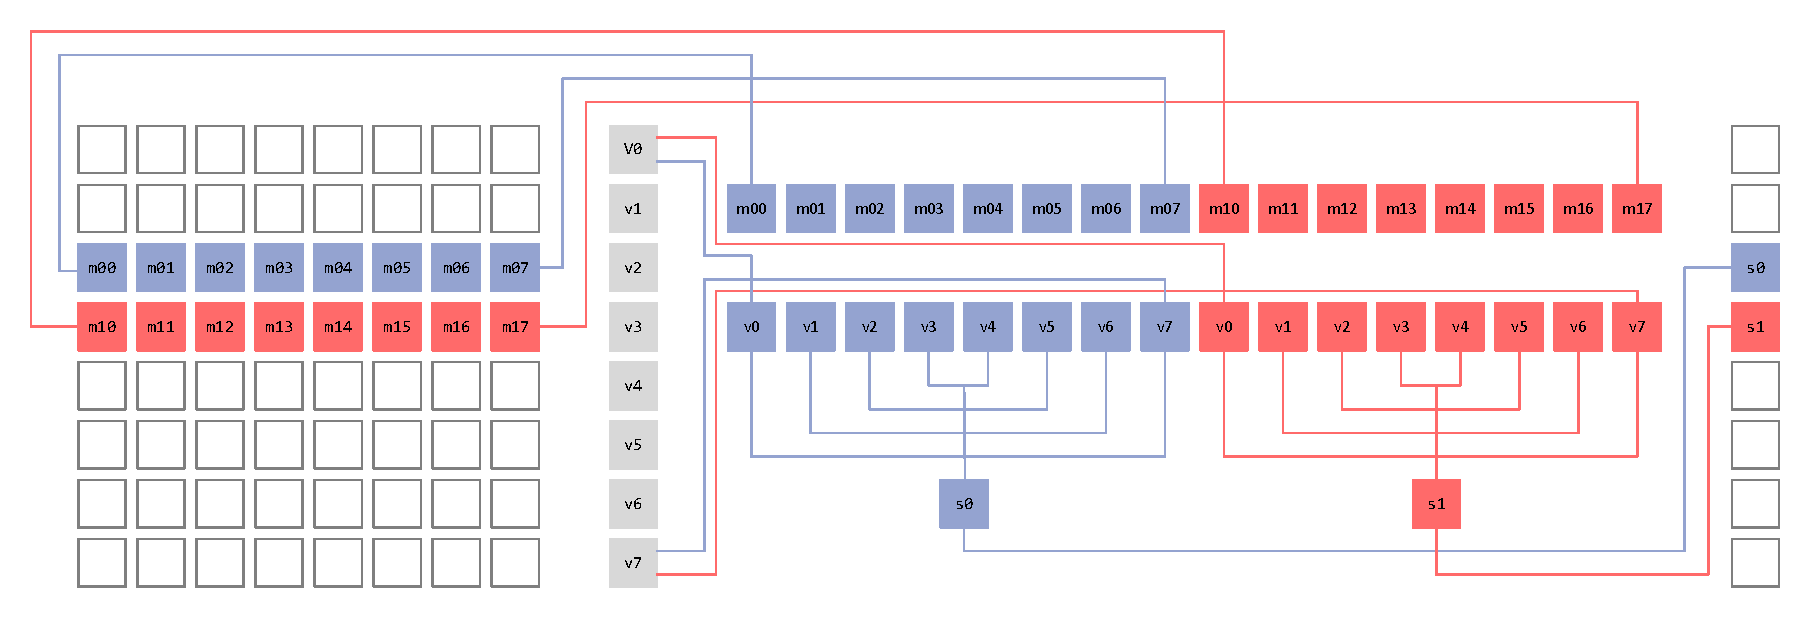
\includegraphics[width=1.0\textwidth]{./fig/vec_matvec8.pdf}
\singlespacing
\captionstyle{center}\caption{Схема вычисления результата в операции \texttt{matvec8}.}
\label{fig:text_4_small_matr_matvec8}
\end{figure}

Итак, при реализации операции умножения матрицы $8 \times 8$ на вектор мы должны загрузить всю матрицу в четыре zmm регистра.
Затем выполнить четыре упакованные операции умножения этих регистров, на регистр, содержащий две копии вектора, на которые умножается матрица.
После этого из каждого из получившихся четырех регистров мы должны получить сумму элементов каждой его половины, что в результате даст 8 искомых элементов выходного вектора.
Получение суммы элементов половины zmm регистра представляет собой горизонтальную операцию, реализация которой с помощью интринсика оказывается слишком дорогой.
Как показали эксперименты, простое применение интринсика \texttt{\_mm512\_mask\_reduce\_add\_ps} (и даже безмасочного \texttt{\_mm512\_reduce\_add\_ps} в случае умножения матрицы $16 \times 16$) не приводит к ускорению по сравнению с оригинальной версией функции, оптимизированной компилятором icc с использованием уровня оптимизации -O3.
Прежде чем переходить к оптимизации горизонтальных операций сложения рассмотрим второй интересующий нас пример, -- перемножение двух матриц размера $8 \times 8$, -- с целью выделения похожих однотипных операций.

Как и в случае с примером умножения матрицы на вектор, вначале приведем простую реализацию неоптимизированной версии перемножения двух матриц размера $8 \times 8$ (листинг~\ref{lst:text_4_small_matr_8x8_mul_matr_noopt}):

Логика перемножения двух матриц состоит в том, что результаты попарного скалярного произведения 8 строк матрицы $a$ и 8 столбцов матрицы $b$ формируют элементы результирующей матрицы.
Как и в случае умножения матрицы на вектор, использование 512-битных команд загрузки данных из памяти позволяет за одну операцию загрузить две соседние строки матрицы $a$ (операцией последовательного чтения) или два соседних столбца матрицы $b$ (с помощью операции gather).
После этого мы должны вычислить четыре скалярные произведения каждой половины загруженного из матрицы $a$ вектора с каждой половиной загруженного из матрицы $b$ вектора.
Для этого выполняются две операции поэлементного перемножения двух загруженных векторов, в одном из которых старшая и младшая половины второго вектора переставлены местами, как показано на рис.~\ref{fig:text_4_small_matr_matmat8}.

\begin{singlespace}
\begin{lstlisting}[caption={Невекторизованная версия перемножения матриц \\ размера $8 \times 8$.}, label={lst:text_4_small_matr_8x8_mul_matr_noopt}]
void matmat8_orig(float* __restrict a,
                  float* __restrict b,
                  float* __restrict r)
{
    for (int i = 0; i < V8; ++i)
    {
        int ii = i * V8;
 
        for (int j = 0; j < V8; ++j)
        {
            float sum = 0.0;

            for (int k = 0; k < V8; ++k)
            {
                int kk = k * V8;
                
                sum = sum + a[ii + k] * b[kk + j];
            }

            r[ii + j] = sum;
        }
    }
}
\end{lstlisting}
\end{singlespace}

\begin{figure}[ht]
\centering
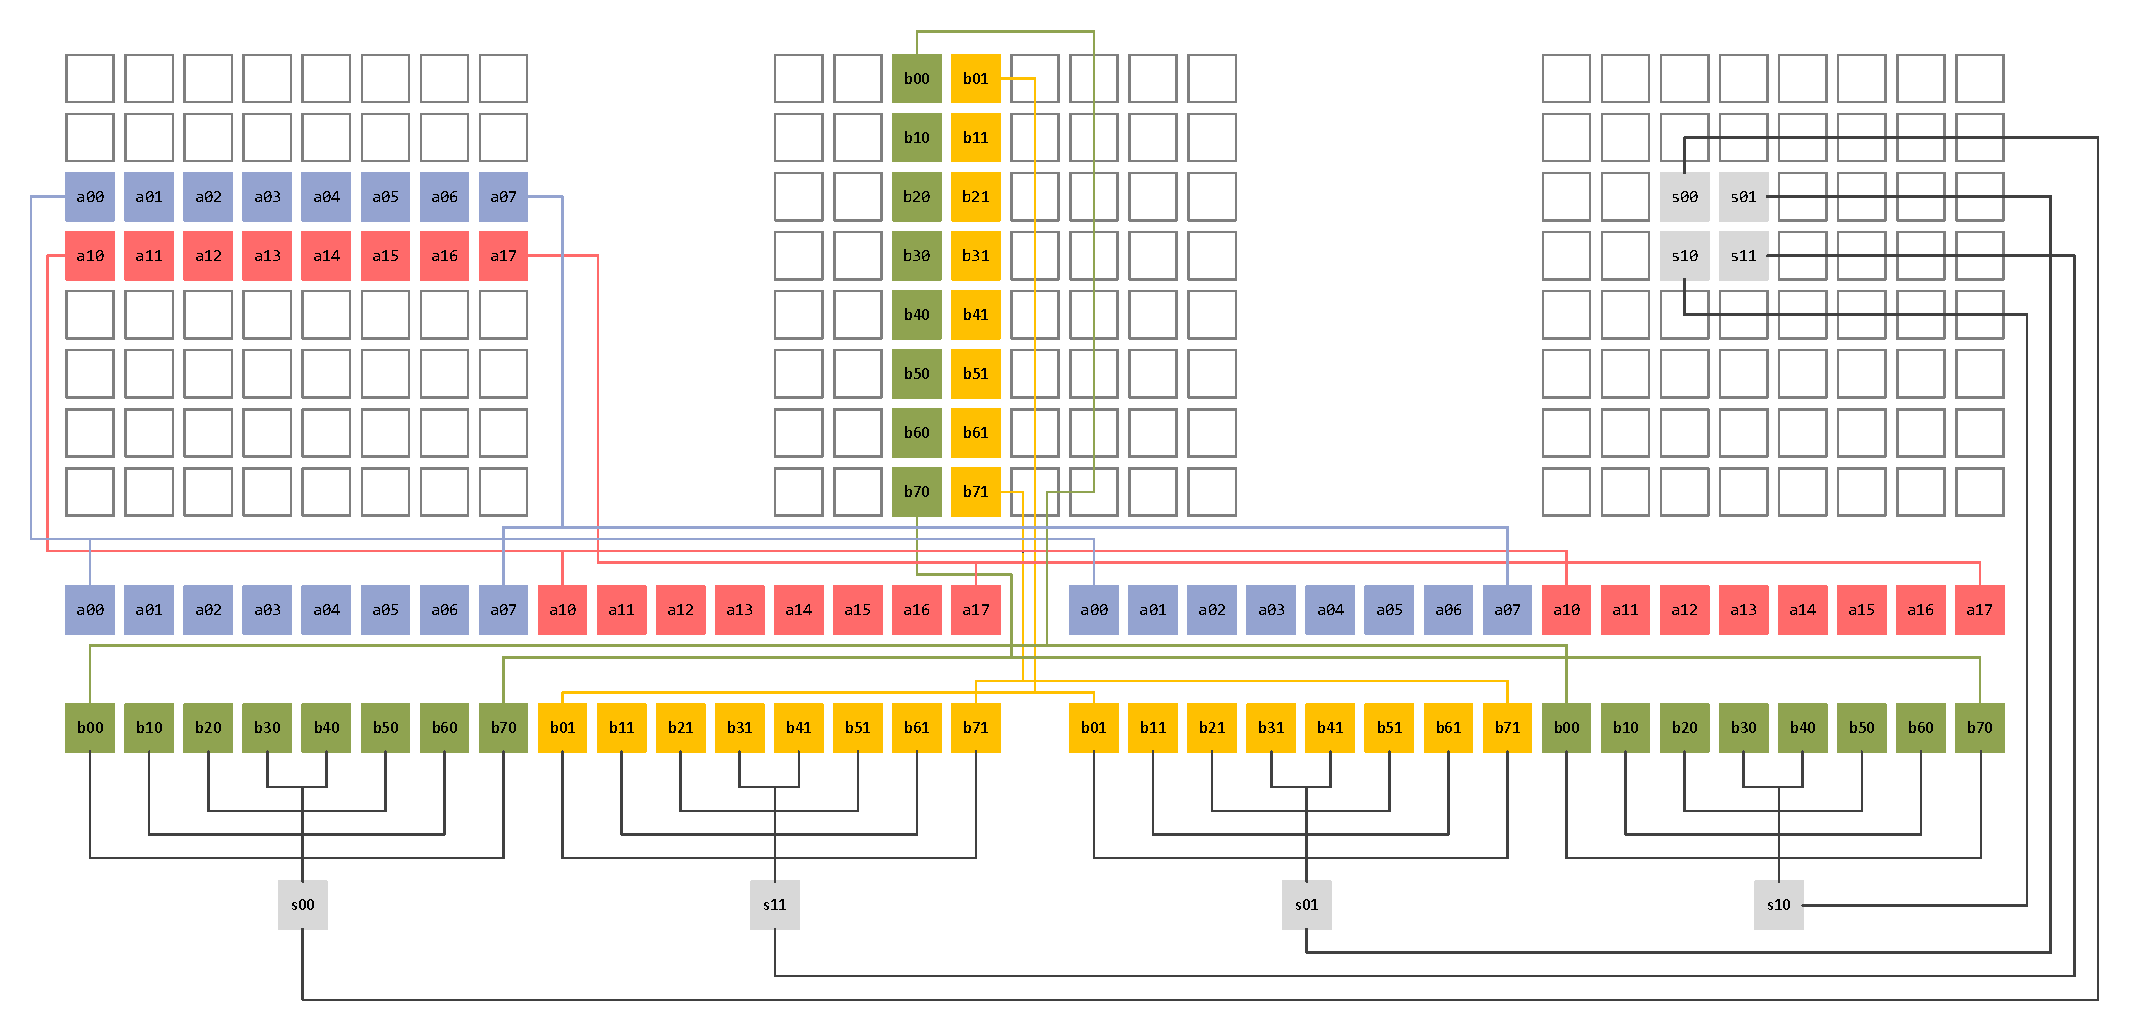
\includegraphics[width=1.00\textwidth]{./fig/vec_matmat8.pdf}
\singlespacing
\captionstyle{center}\caption{Схема вычисления результата в операции \texttt{matmat8}.}
\label{fig:text_4_small_matr_matmat8}
\end{figure}

После выполнения действий, представленных на рис.~\ref{fig:text_4_small_matr_matmat8}, возникает потребность вычисления суммы 8 младших элементов вектора и 8 старших элементов этого же вектора.
Таким образом, мы приходим к тому, что каждый элемент результирующей матрицы должен быть получен с помощью горизонтальной операции суммирования 8 младших или старших элементов некоторого zmm регистра.

Примеры реализаций функций \texttt{matvec16\_orig} и \texttt{matmat16\_orig} аналогичны, но там возникают задачи суммирования всех 16 элементов вектора.
Отсюда возникает потребность объединения таких горизонтальных операций вместе.
Рассмотрим задачу в общем виде: даны 16 zmm регистров (a, b, c, d, e, f, g, h, i, j, k, l, m, n, o, p), каждый из которых содержит по 16 элементов типа float.
Требуется посчитать суммы их элементов и записать в один регистр zmm.
Набор команд AVX-512\label{abbr:avx-7} и библиотека интринсиков содержат все необходимые возможности для эффективной реализации этого функционала.
Схема вычислений состоит из четырех фаз, каждая из которых реализуется операциями перестановок с последующим сложением и слиянием векторов.

\begin{figure}[!ht]
\centering
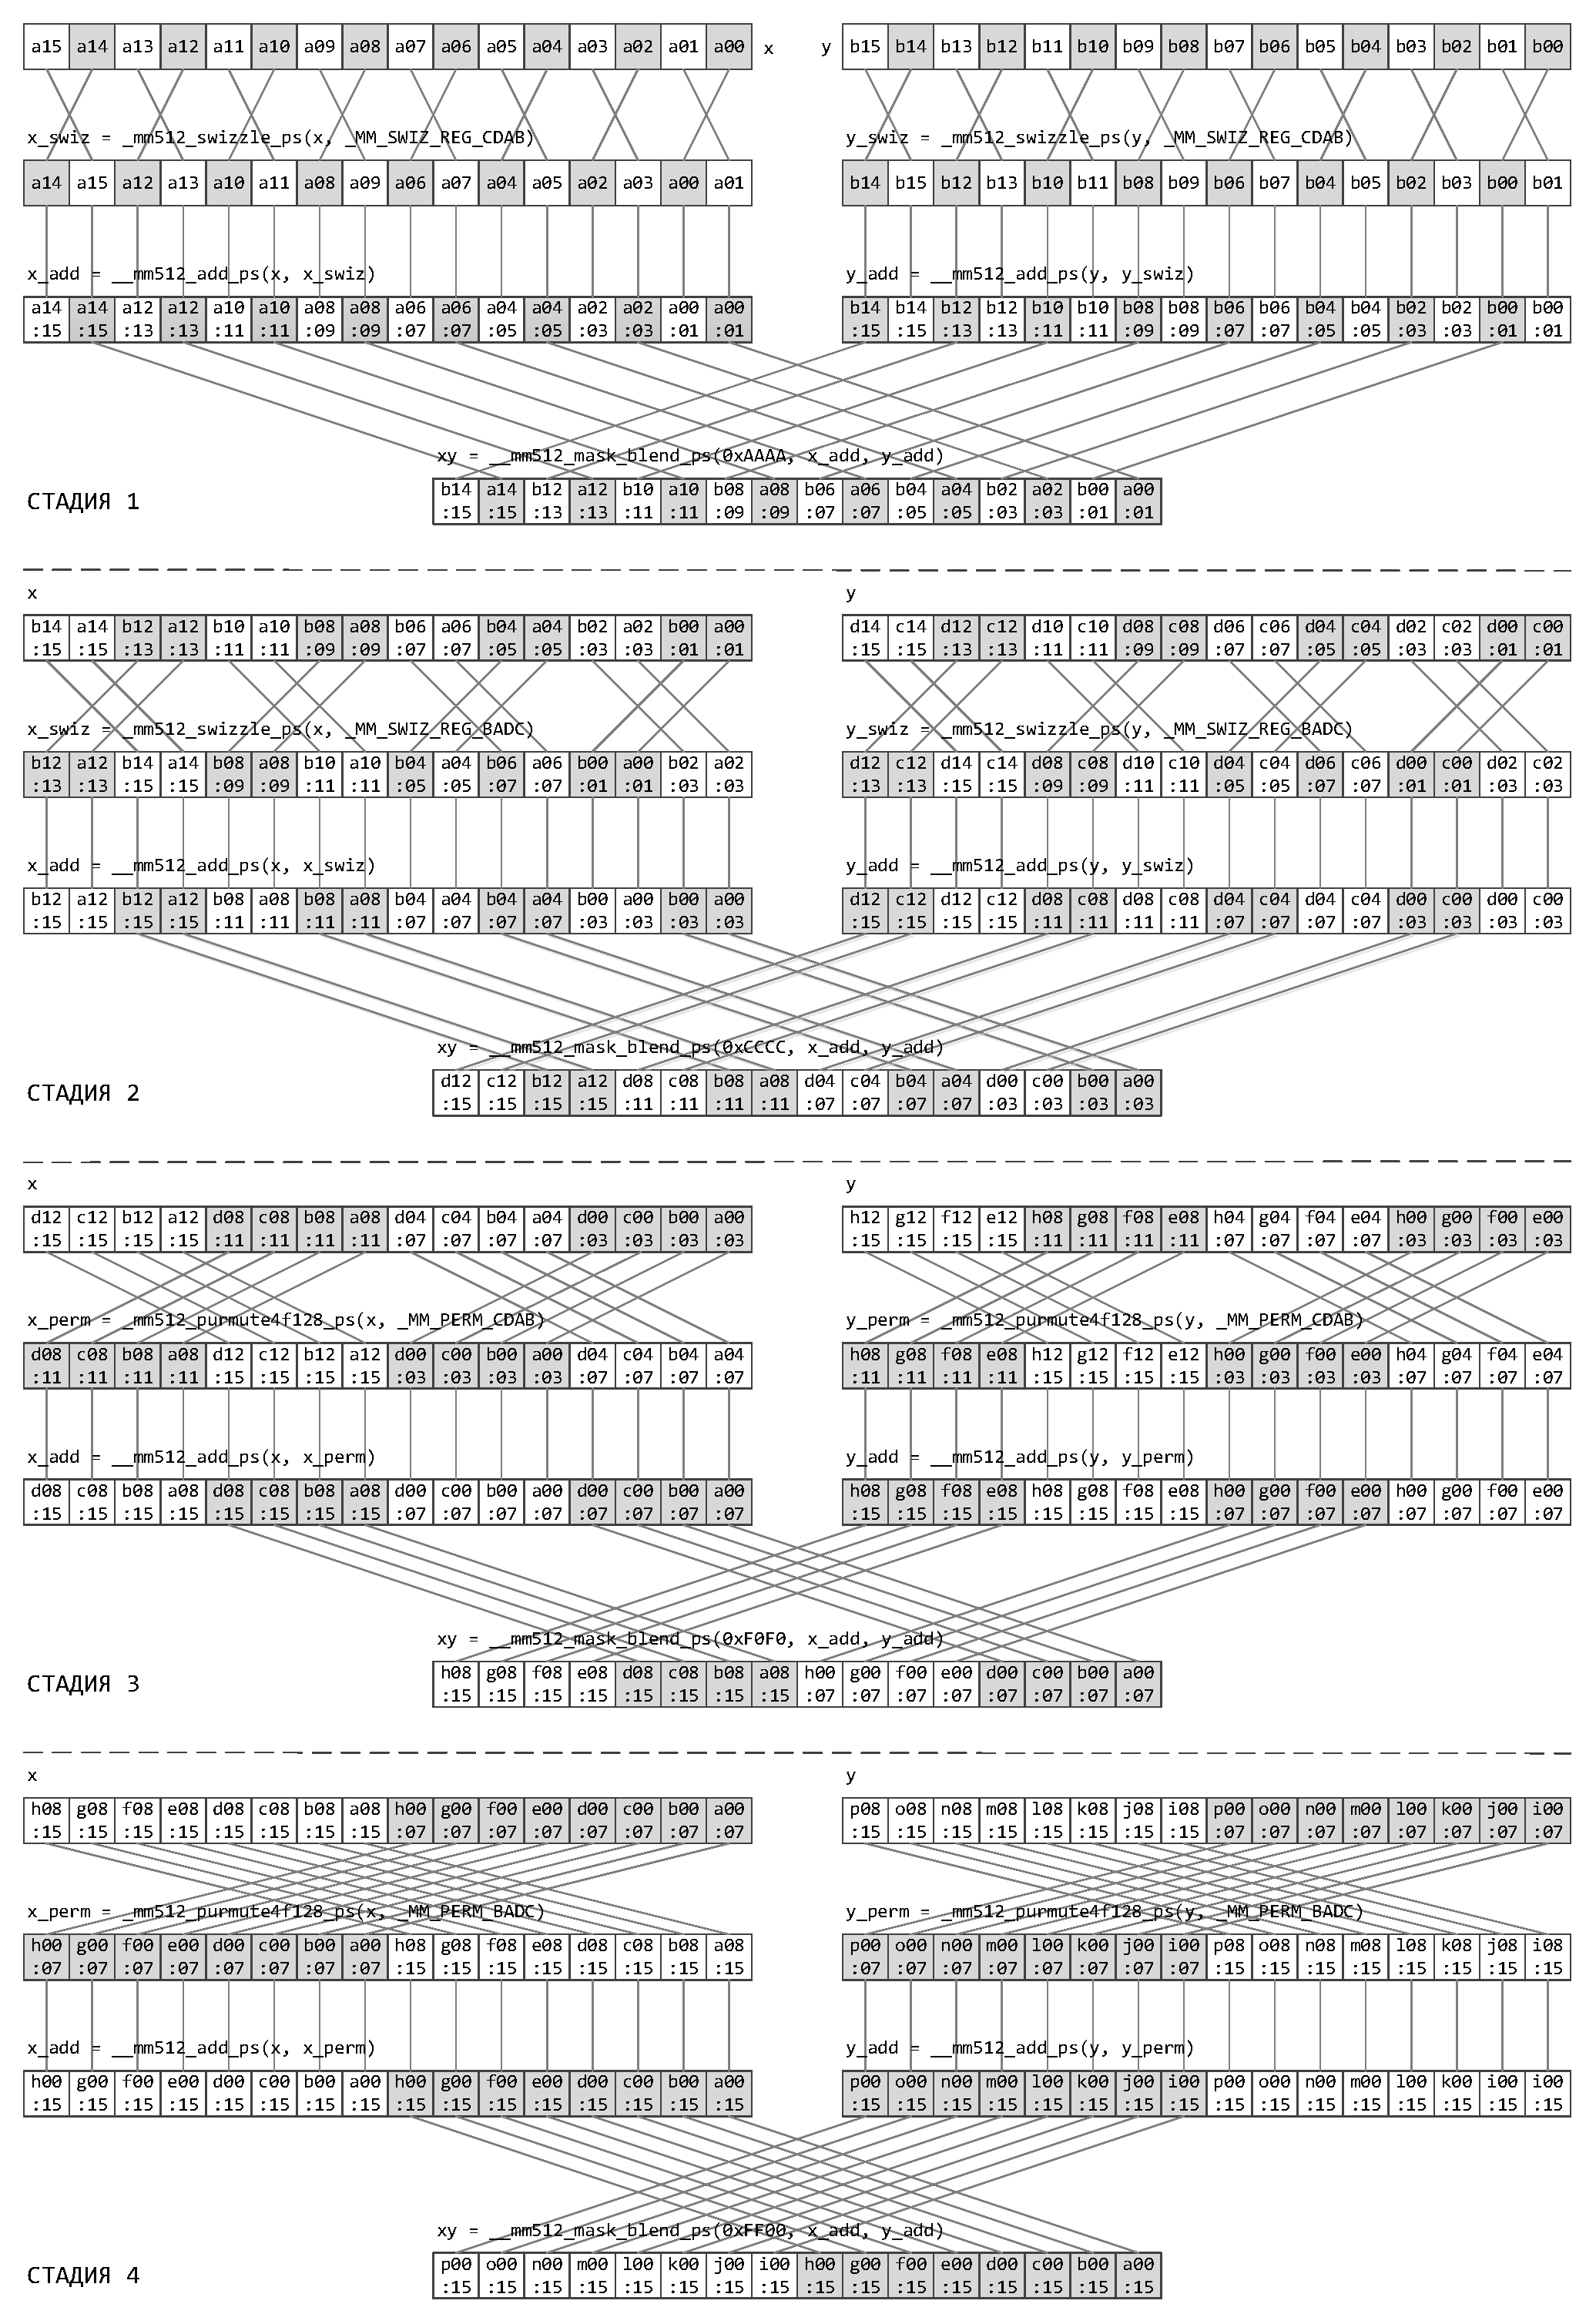
\includegraphics[width=0.95\textwidth]{./fig/vec_horizontal_add.pdf}
\singlespacing
\captionstyle{center}\caption{Схема суммирования элементов zmm вектора.}
\label{fig:text_4_small_matr_horizontal_add}
\end{figure}

На рис.~\ref{fig:text_4_small_matr_horizontal_add} представлена схема суммирования элементов для пары векторов.
Набор команд AVX-512 не содержит операций горизонтального сложения элементов вектора zmm.
Таким образом, для сложения двух элементов одного и того же вектора требуется покомпонентно сложить этот вектор со своей копией, в которой элементы переставлены нужным образом.
Это действие и выполняется на каждой обозначенной на рис.~\ref{fig:text_4_small_matr_horizontal_add} фазе.
Так как всего вектор содержит 16 элементов, то минимальное количество фаз, необходымых для суммирования его элементов равно 4.
После первой фазы (после выполнения операции слияния blend) можно наблюдать вектор, содержащий суммы пар соседних элементов векторов a и b, после второй фазы вектор состоит уже из сумм четверок элементов векторов a, b, c и d, и т. д.

\begin{figure}[ht]
\centering
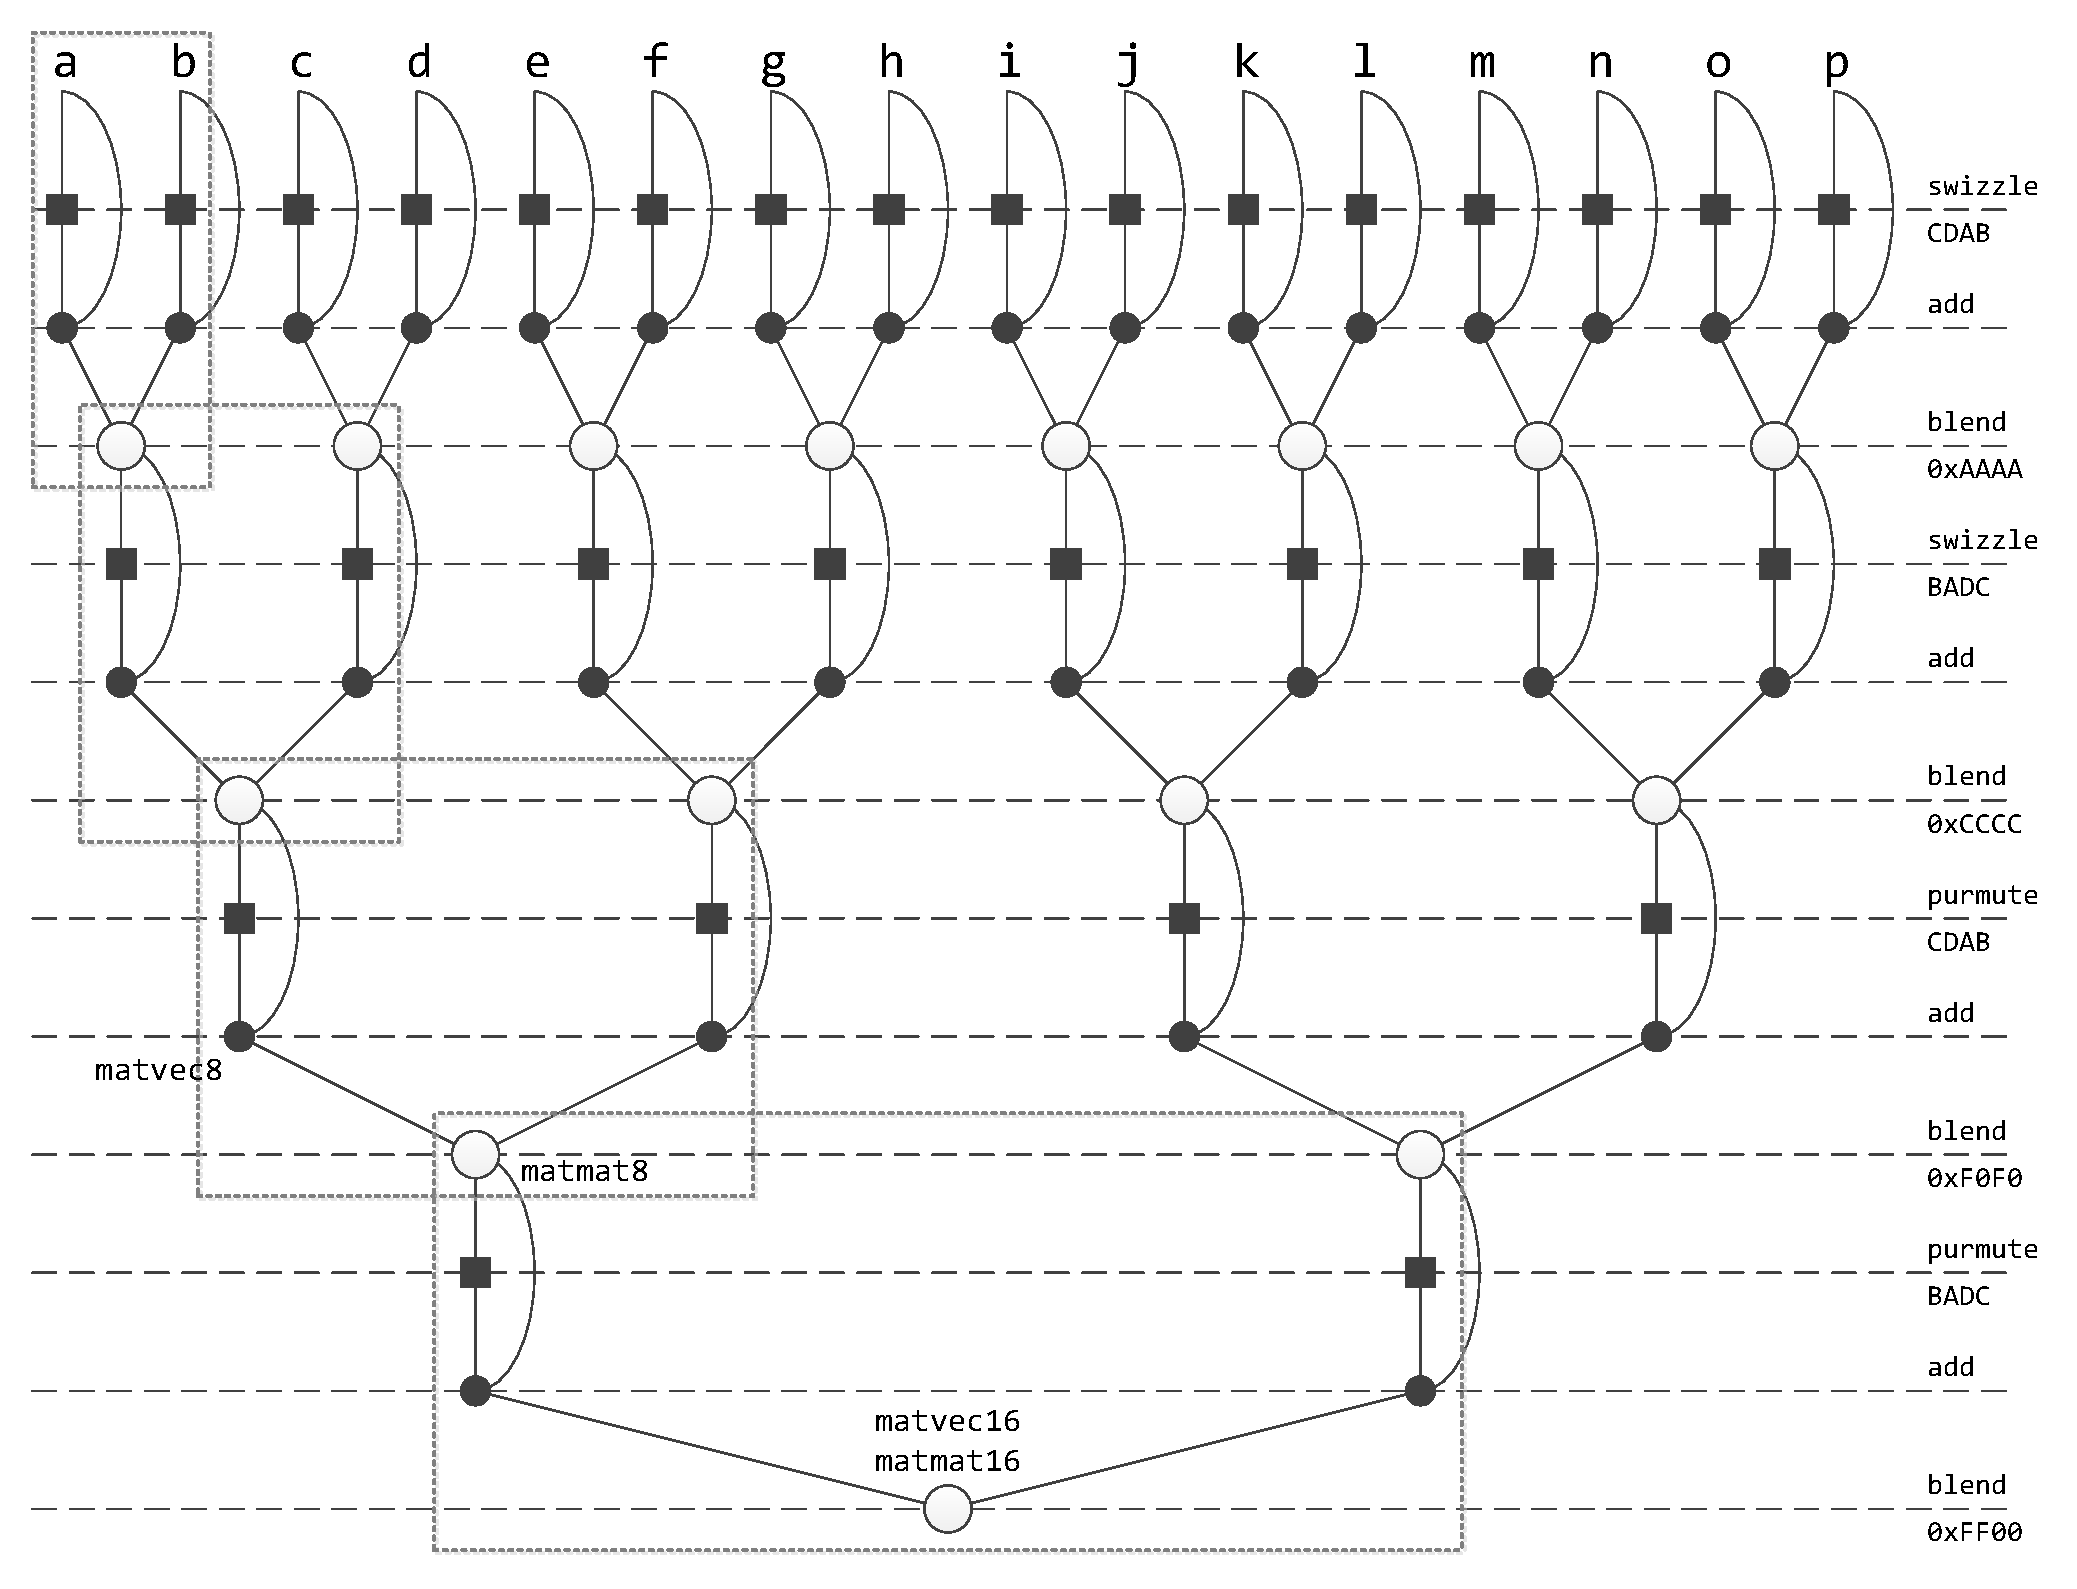
\includegraphics[width=1.0\textwidth]{./fig/vec_horizontal_add_operations_tree.pdf}
\singlespacing
\captionstyle{center}\caption{Схема суммирования элементов 16 zmm векторов.}
\label{fig:text_4_small_matr_operations_tree}
\end{figure}

На рис~\ref{fig:text_4_small_matr_operations_tree} представлен граф потока данных для суммирования всех элементов 16 векторов.
Черными квадратами обозначены операции перестановки элементов (swizzle или permute в терминах интринсиков), черными кругами -- операции сложения вектора со своей пермутированной копией, а белые круги обозначают операции слияния двух векторов по маске.
Прямоугольниками с пунктирной границей очерчены стадии из рис.~\ref{fig:text_4_small_matr_horizontal_add}.

Можно заметить, что граф потока данных на рис.~\ref{fig:text_4_small_matr_operations_tree} состоит из схожих блоков операций, выполняющих одни и те же действия с разными входными регистрами: пермутация двух векторов, сложение пары векторов с пермутированной копией и слияние этих двух результатов по маске (2 swizzle/permute + 2 add + 1 blend).
Причем на каждой фазе свои маски перестановок и слияний, но они постоянны для всех входных векторов.
Для удобства можно определить макросы, реализующие обозначенные фазы.
На вход макрос получает пару обрабатываемых векторов, а также параметры перестановки элементов и слияния результирующей пары.
Пара макросов объясняется тем, что интринсик swizzle предназначен для перестановки элементов внутри 128-битных четвертей, а permute4f128 переставляет местами эти четверти (обе функции раскрываются в операцию perm).

\begin{singlespace}
\begin{lstlisting}[caption={Определение макросов для реализации фаз суммирования элементов векторов.}, label={lst:text_4_small_matr_swiz_macro}]
#define SWIZ_2_ADD_2_BLEND_1(X, Y, SWIZ_TYPE, BLEND_MASK)\
    _mm512_mask_blend_ps(BLEND_MASK,\
        _mm512_add_ps(X, _mm512_swizzle_ps(X, SWIZ_TYPE)),\
        _mm512_add_ps(Y, _mm512_swizzle_ps(Y, SWIZ_TYPE)))

#define PERM_2_ADD_2_BLEND_1(X, Y, PERM_TYPE, BLEND_MASK)\
    _mm512_mask_blend_ps(BLEND_MASK,\
        _mm512_add_ps(X, _mm512_permute4f128_ps(X, PERM_TYPE)),\
        _mm512_add_ps(Y, _mm512_permute4f128_ps(Y, PERM_TYPE)))
\end{lstlisting}
\end{singlespace}

Последний рассматриваемый в разделе пример -- нахождение обратной матрицы с помощью алгоритма Гаусса-Жордана \texttt{invmat8\_orig}.
По алгоритму Гаусса-Жордана к исходной матрице $m$ нужно приписать справа единичную матрицу $e$.
Получим прямоугольную матрицу вида ($m|e$), размера $8 \times 16$.
Далее над этой матрицей необходимо выполнить такие преобразования строк (перестановка строк, умножение строки на число, прибавление одной строки к другой), чтобы исходная матрица, стоящая слева, трансформировалась в единичную.
Тогда матрица, стоящая справа, из единичной трансформируется в искомую обратную матрицу.
Действия выполняются над строками матрицы размера $8 \times 16$, последовательно хранящейся в памяти.
Так как на вход функции подается матрица $8 \times 8$, также хранящаяся в памяти последовательно, то внутри функции возникают накладные действия, связанные с копированием элементов входной матрицы во временную матрицу $8 \times 16$ и обратным копированием из временной матрицы результата.
Также требуется инициализация правой части временной матрицы элементами единичной матрицы.
Все эти накладные действия реализуются с помощью операций gather/scatter.
Заметим, что при реализации \texttt{invmat16} накладные расходы отсутствуют.

\subsubsection{Векторизация операций с малоразмерными \mbox{матрицами}}\label{sec:text_4_small_matr_realization}

В реализации функции \texttt{matvec8\_opt} следует отметить загрузку двух копий вектора в zmm регистр с помощью операции gather.
Существует возможность загрузки двух копий 256-битного участка памяти в zmm регистр, однако реализована она с помощью функции-интринсика \texttt{\_mm512\_extload\_pd} с указанием параметра \texttt{\_MM\_BROADCAST\_4X8}.
Так как формально результатом является регистр типа \texttt{\_\_m512d}, то было решено оставить чтение через gather.
Суммирование половинок четырех zmm регистров заканчивается на операции add третьей фазы, как показано на рис.~\ref{fig:text_4_small_matr_horizontal_add} (см. листинг~\ref{lst:text4_small_matr_matvec_opt}).

\begin{singlespace}
\begin{lstlisting}[caption={Векторизованная версия умножения матрицы \\ размера $8 \times 8$ на вектор.}, label={lst:text4_small_matr_matvec_opt}]
void matvec8_opt(float* __restrict m,
                 float* __restrict v,
                 float* __restrict r)
{
  ...
  ind_gth = _mm512_set_epi32(7,6,5,4,3,2,1,0,7,6,5,4,3,2,1,0);
  ind_sct = _mm512_set_epi32(0,0,0,0,7,5,3,1,0,0,0,0,6,4,2,0);
  ...
  vec = _mm512_i32gather_ps(ind_gth, v, _MM_SCALE_4);
  ...
  m0 = _mm512_mul_ps(_mm512_load_ps(&m[0]), vec);
  ...
  x0 = SWIZ_2_ADD_2_BLEND_1(m0, m2, _MM_SWIZ_REG_CDAB, 0xAAAA);
  x2 = SWIZ_2_ADD_2_BLEND_1(m4, m6, _MM_SWIZ_REG_CDAB, 0xAAAA);
  m0 = SWIZ_2_ADD_2_BLEND_1(x0, x2, _MM_SWIZ_REG_BADC, 0xCCCC);
  x0 = _mm512_add_ps(m0, _mm512_permute4f128_ps(m0, _MM_PERM_CDAB));
  ...
  _mm512_mask_i32scatter_ps(r, 0xF0F, ind_sct, x0, _MM_SCALE_4);
}
\end{lstlisting}
\end{singlespace}

Перемножение двух матриц изначально реализуется гнездом из трех вложенных циклов.
Два внешних цикла относятся к проходу по строкам одной из перемножаемых матриц и столбцам другой.
Во внутреннем цикле вычисляется скалярное произведение соответствующей строки и столбца.
Чтение двух соседних строк выполняется обычной функцией \texttt{\_mm512\_load\_ps}.
Загрузка двух соседних столбцов выполняется с помощью gather и заданными смещениями всех элементов.
По этой причине в реализации была выполнена перестановка двух внешних циклов, чтобы чтение с помощью gather выполнялось во внешнем цикле.
Далее выполняется полная раскрутка ставшего теперь уже внутренним цикла, проходящего по строкам матрицы $a$.
Суммирование половинок 8 регистров zmm заканчивается на операции blend третьей фазы из рис.~\ref{fig:text_4_small_matr_horizontal_add}.
Полученные 16 элементов результирующей матрицы записываются в память с использованием scatter с указанием смещений (см. листинг~\ref{lst:text_4_small_matr_matmat_opt}).

\begin{singlespace}
\begin{lstlisting}[caption={Векторизованная версия перемножения \ \\ матриц размера $8 \times 8$.}, label={lst:text_4_small_matr_matmat_opt}]
void matmat8_opt(float* __restrict a,
                 float* __restrict b,
                 float* __restrict r)
{
 ...
 ind = _mm512_set_epi32(7*V8+1, 6*V8+1, 5*V8+1, 4*V8+1,
                        3*V8+1, 2*V8+1,   V8+1,      1,
                        7*V8,   6*V8,   5*V8,   4*V8,
                        3*V8,   2*V8,     V8,        0);

 for (int j = 0; j < V8; j += 2)
 {
  ...
  bj = _mm512_i32gather_ps(ind, &b[j], _MM_SCALE_4);
  bj2 = _mm512_permute4f128_ps(bj, _MM_PERM_BADC);
  ...
  a0 = _mm512_load_ps(&a[ii0]);
  m0 = _mm512_mul_ps(a0, bj);
  m1 = _mm512_mul_ps(a0, bj2);
  ...
  x0 = SWIZ_2_ADD_2_BLEND_1(m0, m1, _MM_SWIZ_REG_CDAB, 0xAAAA);
  x1 = SWIZ_2_ADD_2_BLEND_1(m2, m3, _MM_SWIZ_REG_CDAB, 0xAAAA);
  x2 = SWIZ_2_ADD_2_BLEND_1(m4, m5, _MM_SWIZ_REG_CDAB, 0xAAAA);
  x3 = SWIZ_2_ADD_2_BLEND_1(m6, m7, _MM_SWIZ_REG_CDAB, 0xAAAA);
  m0 = SWIZ_2_ADD_2_BLEND_1(x0, x1, _MM_SWIZ_REG_BADC, 0xCCCC);
  m1 = SWIZ_2_ADD_2_BLEND_1(x2, x3, _MM_SWIZ_REG_BADC, 0xCCCC);
  x0 = PERM_2_ADD_2_BLEND_1(m0, m1, _MM_PERM_CDAB, 0xF0F0);
  ...
  ind1 = _mm512_set_epi32(ii3+V8+j, ii3+V8+j+1,
                          ii2+V8+j, ii2+V8+j+1,
                          ii1+V8+j, ii1+V8+j+1,
                          ii0+V8+j, ii0+V8+j+1,
                          ii3+j+1,  ii3+j,
                          ii2+j+1,  ii2+j,
                          ii1+j+1,  ii1+j,
                          ii0+j+1,  ii0+j),
  _mm512_i32scatter_ps(r, ind1, x0, _MM_SCALE_4);
}
\end{lstlisting}
\end{singlespace}

Реализация функции \texttt{invmat8\_opt} начинается с формирования временной матрицы размера $8 \times 16$.
После инициализации временной матрицы выполняется тело алгоритма Гаусса-Жордана нахождения обратной матрицы.
Действие по нахождению ведущей строки не подвергалось векторизации.
Три остальные действия реализуются без каких бы то ни было особенностей с помощью применения пересылок и покомпонентных операций сложения, умножения и комбинированных FMA\label{abbr:fma-2} операций.

\begin{singlespace}
\begin{lstlisting}[caption={Векторизованная версия вычисления обратной \\ матрицы размера $8 \times 8$.},label={lst:text_4_small_matr_invmat_opt}]
int invmat8_opt(float* __restrict m, float* __restrict r)
{
  z0 = _mm512_setzero_ps();
  z1 = _mm512_set1_ps(1.0);
  ind1 = _mm512_set_epi32(V16+7,V16+6,V16+5,V16+4,V16+3,V16+2,V16+1,V16,
                          7,6,5,4,3,2,1,0);
  ind2 = _mm512_set_epi32(0,0,0,0,0,0,0,0,
                          7*V16+7,6*V16+6,5*V16+5,4*V16+4,
                          3*V16+3,2*V16+2,V16+1,0);

  for (int i = 0; i < V8; i += 2)
  {
    _mm512_i32scatter_ps(&t[i * V16], ind1, _mm512_load_ps(&m[i * V8]),
                         _MM_SCALE_4);
    _mm512_i32scatter_ps(&t[i * V16 + V8], ind1, z0, _MM_SCALE_4);
  }

  _mm512_mask_i32scatter_ps(&t[V8], 0xFF, ind2, z1, _MM_SCALE_4);

  for (int i = 0; i < V8; ++i)
  {
    ...
    if (lead_i != i)
    {
      vi = _mm512_load_ps(&t[ii]);
      vl = _mm512_load_ps(&t[lead_i * V16]);
      _mm512_store_ps(&t[lead_i * V16], vi);
      _mm512_store_ps(&t[ii], vl);
    }
    ...
    vd = _mm512_set1_ps(1.0 / t[ii + i]);
    vi = _mm512_load_ps(&t[ii]);
    vi = _mm512_mul_ps(vi, vd);
    _mm512_store_ps(&t[ii], vi);
    ...
    for (int j = 0; j < V8; ++j)
    {
      int jj = j * V16;
      if (j != i)
      {
        vd = _mm512_set1_ps(-t[jj + i]);
        vj = _mm512_load_ps(&t[jj]);
        vi = _mm512_load_ps(&t[ii]);
        vj = _mm512_fmadd_ps(vi, vd, vj);
        _mm512_store_ps(&t[jj], vj);
      }
    }
  }

  ...
  for (int i = 0; i < V8; i += 2)
  {
    vi = _mm512_i32gather_ps(ind, &t[i * V16 + V8], _MM_SCALE_4);
    _mm512_store_ps(&r[i * V8], vi);
  }
}
\end{lstlisting}
\end{singlespace}

После завершения работы алгоритма Гаусса-Жордана результат из временной матрицы перемещается в область памяти результата с помощью пар операций gather/store.

Реализация функций по работе с матрицами $16 \times 16$ не приводится, так как эти функции имплементируются аналогично, только код получается более громоздкий.
Выполнение горизонтальных операций сложения для \texttt{matvec16} и \texttt{matmat16} охватывает все четыре фазы из рис.~\ref{fig:text_4_small_matr_horizontal_add}, логика же вычислений более примитивна, так как не требуется объединения итераций при обходе матриц -- одна строка матрицы в точности заполняет zmm регистр.
Полные тексты приведенного в разделе программного кода доступны в \cite{iparGithub}.

Реализованные оптимизированные с помощью инструкций AVX-512 функции для работы с матрицами размера $8 \times 8$ и $16 \times 16$ были опробованы на процессоре Intel Xeon Phi KNL\label{abbr:knl-6}.
Hассматривались два варианта исполняемого кода.
В первом варианте функции были реализованы без использования интринсиков, компилировались с использованием компилятора icc с уровнем оптимизации -O3.
Во втором варианте использовались те же опции компиляции, однако функции были оптимизированы вручную, как это представлено в листингах~\ref{lst:text4_small_matr_matvec_opt}, \ref{lst:text_4_small_matr_matmat_opt}, \ref{lst:text_4_small_matr_invmat_opt}.
В обоих вариантах был запрещен инлайн рассматриваемых функций в место вызова.
Размеры матриц рассматривались в двух вариантах: $8 \times 8$ и $16 \times 16$.
На рис.~\ref{fig:text_4_small_matr_res} приведены данные по ускорению векторизованных версий функций работы с матрицами.

\begin{figure}[ht]
\centering
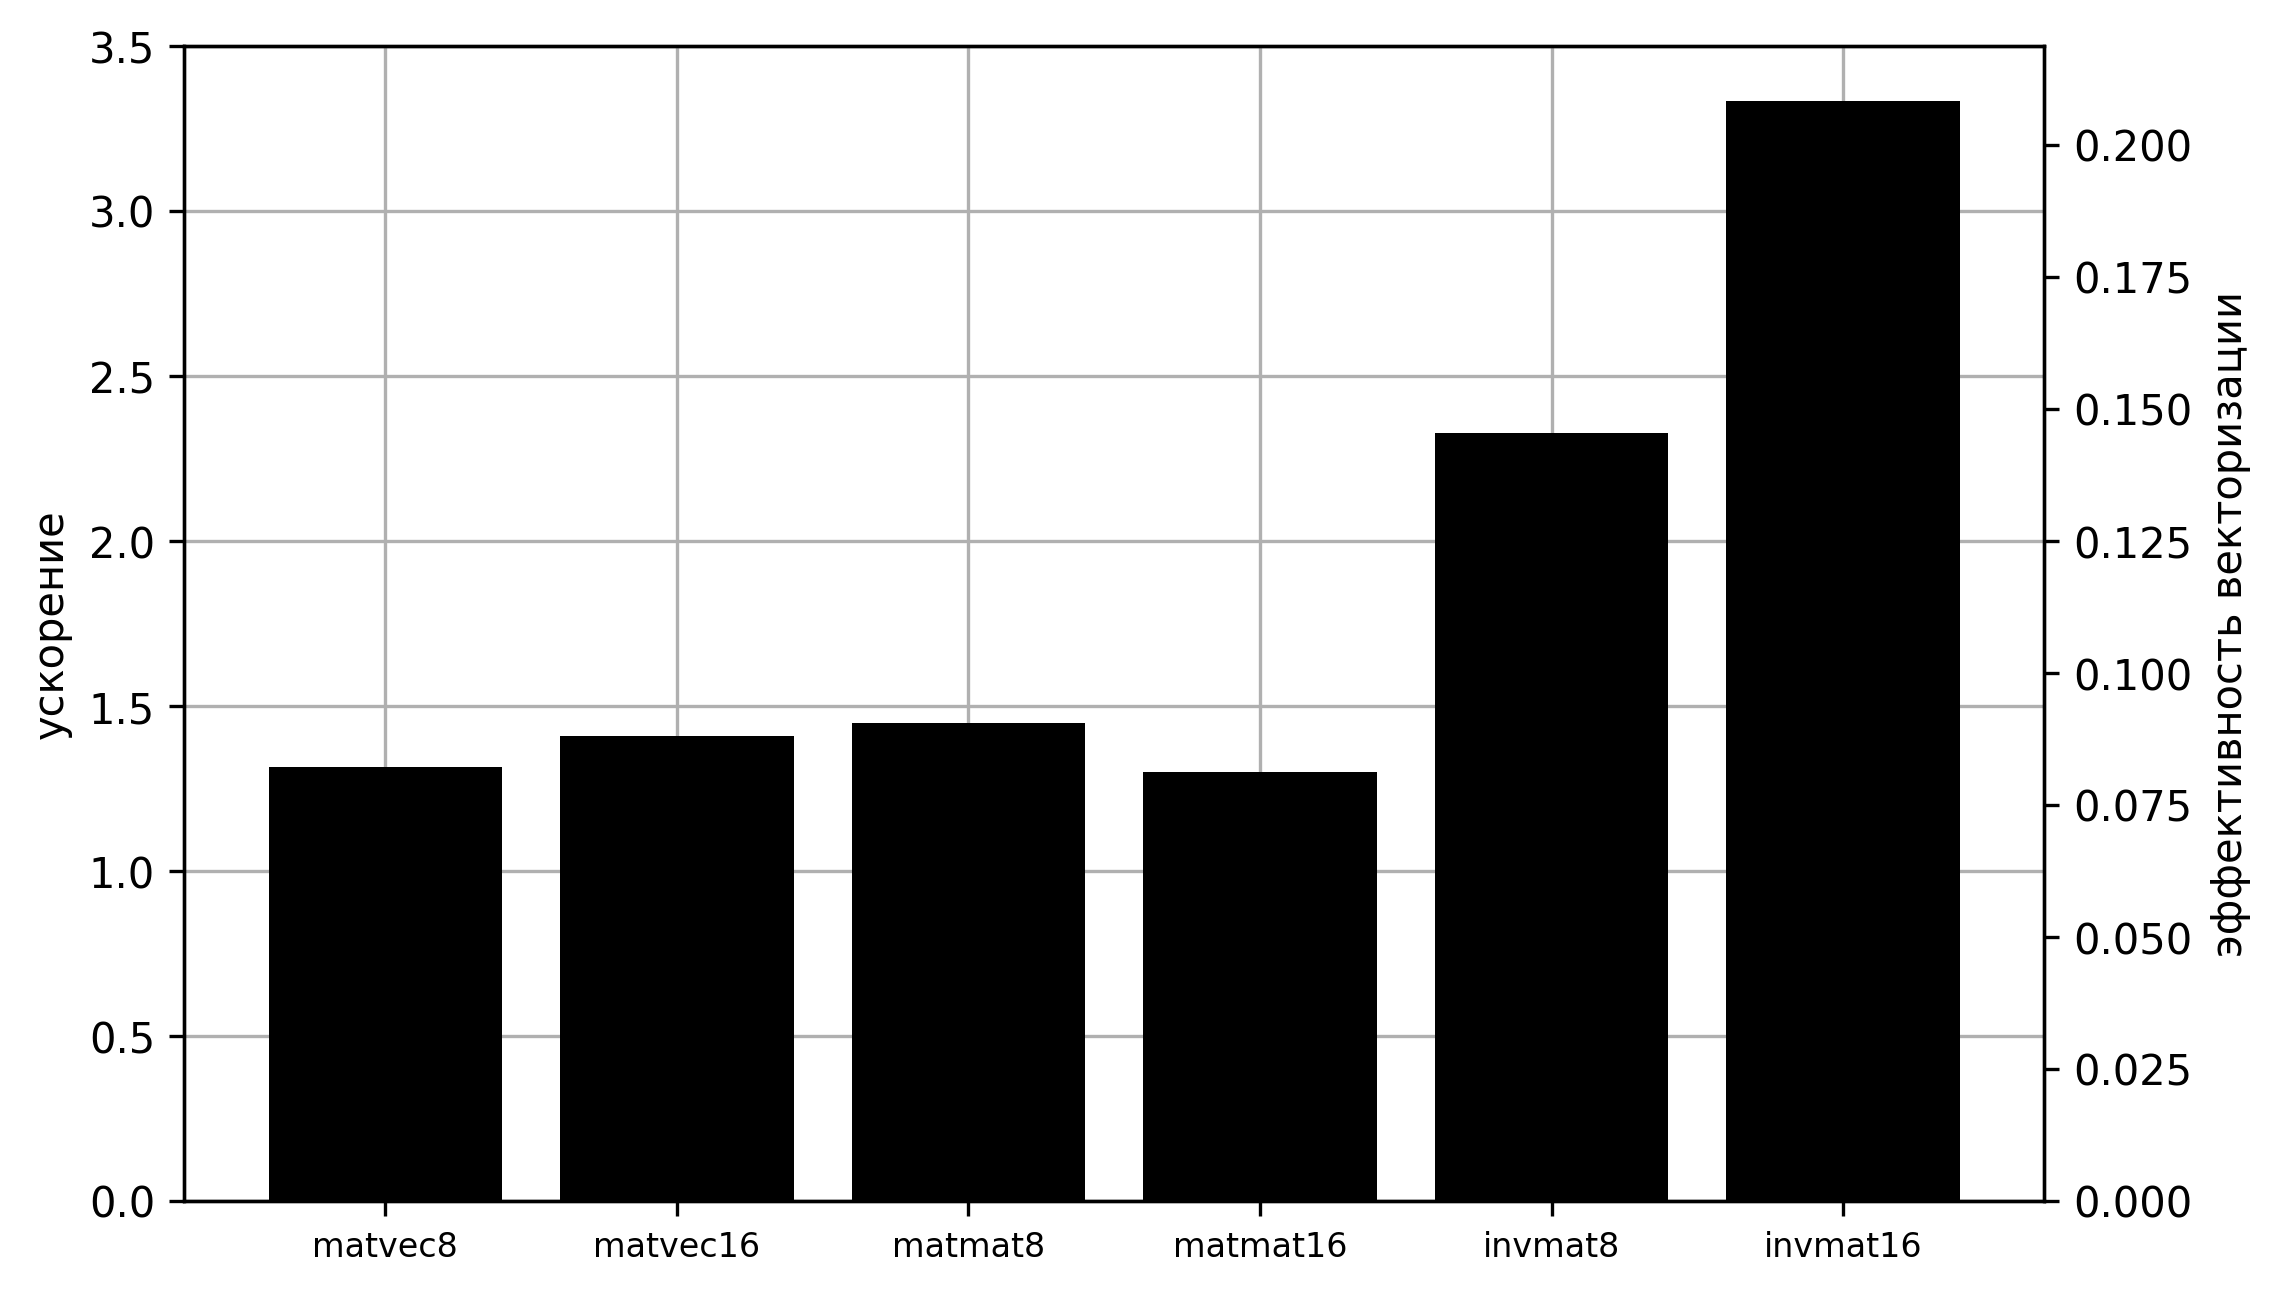
\includegraphics[width=0.6\textwidth]{./fig/vec_small_matr_res.png}
\singlespacing
\captionstyle{center}\caption{Ускорение и эффективность векторизации операций над матрицами размера $8 \times 8$ и $16 \times 16$.}
\label{fig:text_4_small_matr_res}
\end{figure}

Наибольшее ускорение продемонстрировали функции нахождения обратной матрицы, так как алгоритм нахождения обратной матрицы естественным образом формулируется в терминах работы со строками объединенной матрицы, что находит свое отражение в 512-битных векторных операциях.
При этом функция \texttt{invmat16} ускорилась больше, чем \texttt{invmat8} из-за отсутствия накладных расходов.
Функции \texttt{matvec8/16} и \texttt{matmat8/16} демонстрируют умеренное ускорение из-за наличия горизонтальных операций сложения.
Объединение горизонтальных операций позволяет сгладить этот эффект, однако для дальнейшего ускорения требуется реализация объединенных функций, выполняющих одновременно сразу несколько операций или применяющих одну операцию к более широкому набору данных (например, функция перемножение двух пар матриц).

% Векторизация перемножения матриц специального вида.
\subsubsection{Потери производительности из-за неполного \mbox{использования} элементов векторных регистров}\label{sec:text_4_spec_matr}

В разделах~\ref{sec:vec_small_matr_opers} и \ref{sec:text_4_small_matr_realization} рассматривались матрицы размера $8 \times 8$ и $16 \times 16$, работа с которыми удобна в плане векторизации, так как в один векторных регистр помещается ровно 8 значений формата double или 16 значений формата float.
Однако, при работе с другими размерностями неизбежно возникает проблема неполного использования элементов векторных регистров, что приводит к падению производительности.

При проведении вычислений с помощью метода RANS/ILES\label{abbr:rans-3}\label{abbr:iles-3} расчетные параметры компонуются внутри матриц размером $5 \times 5$, эти матрицы являются подматрицами матриц размера $8 \times 8$ (это делается из соображений выровненности расположения в памяти).
Будем рассматривать операцию перемножения таких матриц и возможные пути повышения производительности этой операции \cite{Bendersky2018VecMat1}. 

\begin{figure}[ht]
\centering
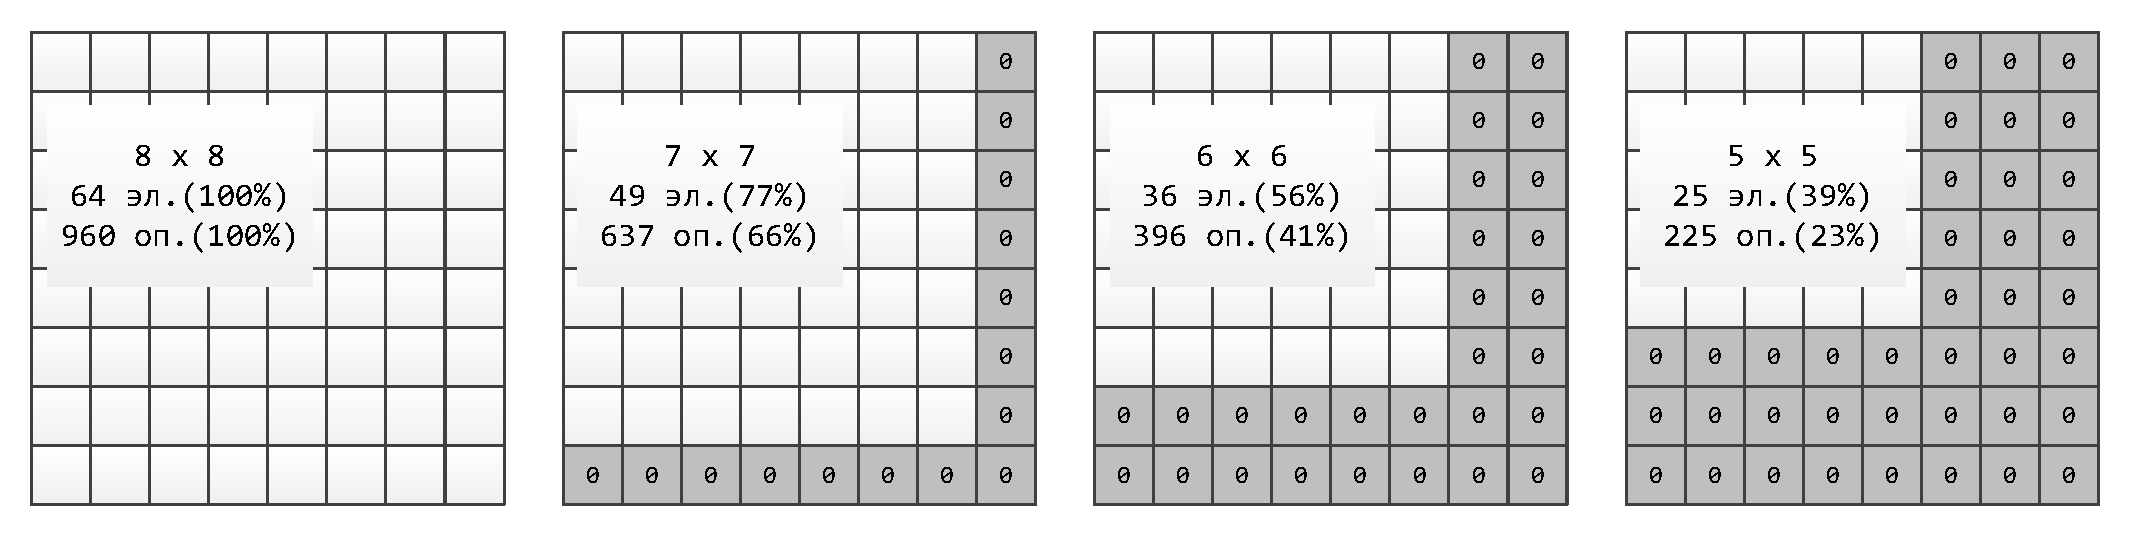
\includegraphics[width=1.00\textwidth]{./fig/vec_spec_matrices.pdf}
\singlespacing
\captionstyle{center}\caption{Иллюстрация матриц размера $8 \times 8$, $7 \times 7$, $6 \times 6$, $5 \times 5$, представленных как подматрицы матрицы $8 \times 8$.}
\label{fig:text_4_spec_matr_matrices}
\end{figure}

Идея выделения однотипных операций из раздела~\ref{sec:text_4_small_matr_realization} обладает существенными недостатками.
Во-первых, в коде присутствуют медленные инструкции gather/scatter.
Во-вторых, выполнение сначала поэлементного перемножения векторов, а затем параллельное нахождение сумм их элементов (в рассматриваемом случае рассчитываются суммы элементов половинок векторов), делают невозможным использование эффективных комбинированных инструкций fmadd.
Рассмотрим пути по устранению перечисленных недостатков.

Запишем в явном виде значения элементов $i$-й строки результирующей матрицы:
\begin{equation}
	\left\{
		\begin{aligned}
			& r_{i0} = a_{i0}b_{00} + a_{i1}b_{10} + \cdots + a_{i7}b_{70} \\
			& \cdots \\
			& r_{i7} = a_{i0}b_{07} + a_{i1}b_{17} + \cdots + a_{i7}b_{77}
		\end{aligned}
	\right.
\end{equation}
или в векторном виде $\overline{r}_i = a_{i0}\overline{b}_0 + a_{i1}\overline{b}_1 + \cdots + a_{i7}\overline{b}_7$, что в объединении с выражением для $i + 1$-ой строки $\overline{r}_{i + 1} = a_{i + 1,0}\overline{b}_0 + a_{i + 1,1}\overline{b}_1 + \cdots + a_{i + 1,7}\overline{b}_7$ приводит к выражению
\begin{equation}\label{eqn:text_4_spec_matr_riip1}
	\overline{r}|_{i + 1}^i
	=
	\sum_{j = 0}^{7} \left(  \overline{a}|_{i + 1,j}^{ij} \circ \overline{b}|_j^j \right),
\end{equation}
где $\overline{r}|_{i + 1}^i$ -- комбинированный вектор состоящий из векторов $\overline{r}_i$ и $\overline{r}_{i + 1}$, $\overline{b}|_j^j$ -- комбинированный вектор состоящий из двух копий вектора $\overline{b}_j$, а $\overline{a}|_{i + 1,j}^{ij}$ -- вектор, первые 8 элементов которого равны $a_{ij}$, а остальные 8 элементов равны $a_{i + 1,j}$.
Получающийся по формуле~\eqref{eqn:text_4_spec_matr_riip1} комбинированный вектор $\overline{r}|_{i + 1}^i$ расположен в памяти последовательно, и записывать его в память можно с помощью интринсика \texttt{\_mm512\_store\_ps}.
При этом предполагаем, что значение $i$ четно, то есть вектор $\overline{r}|_{i + 1}^i$ выровнен в памяти должным образом.
Другие комбинированные векторы в \eqref{eqn:text_4_spec_matr_riip1} получаются с помощью инструкции perm (интринсик \texttt{\_mm512\_permutexvar\_ps}), примененной к соответствующим загруженным соседним строкам матриц $a$ и $b$.
При реализации \eqref{eqn:text_4_spec_matr_riip1} не требуется использование медленных инструкций gather/scatter, так как столбцы матриц не читаются и не записываются (работа ведется только со строками).
После того, как векторы $\overline{a}|_{i + 1,j}^{ij}$ и $\overline{b}|_j^j$ сформированы, нужно выполнить их попарное поэлементное перемножение, после чего сложить в один вектор (8 операций поэлементного умножения, 7 операций сложения).
Эти действия можно выполнить, используя комбинированные операции fmadd.

\begin{figure}[ht]
\centering
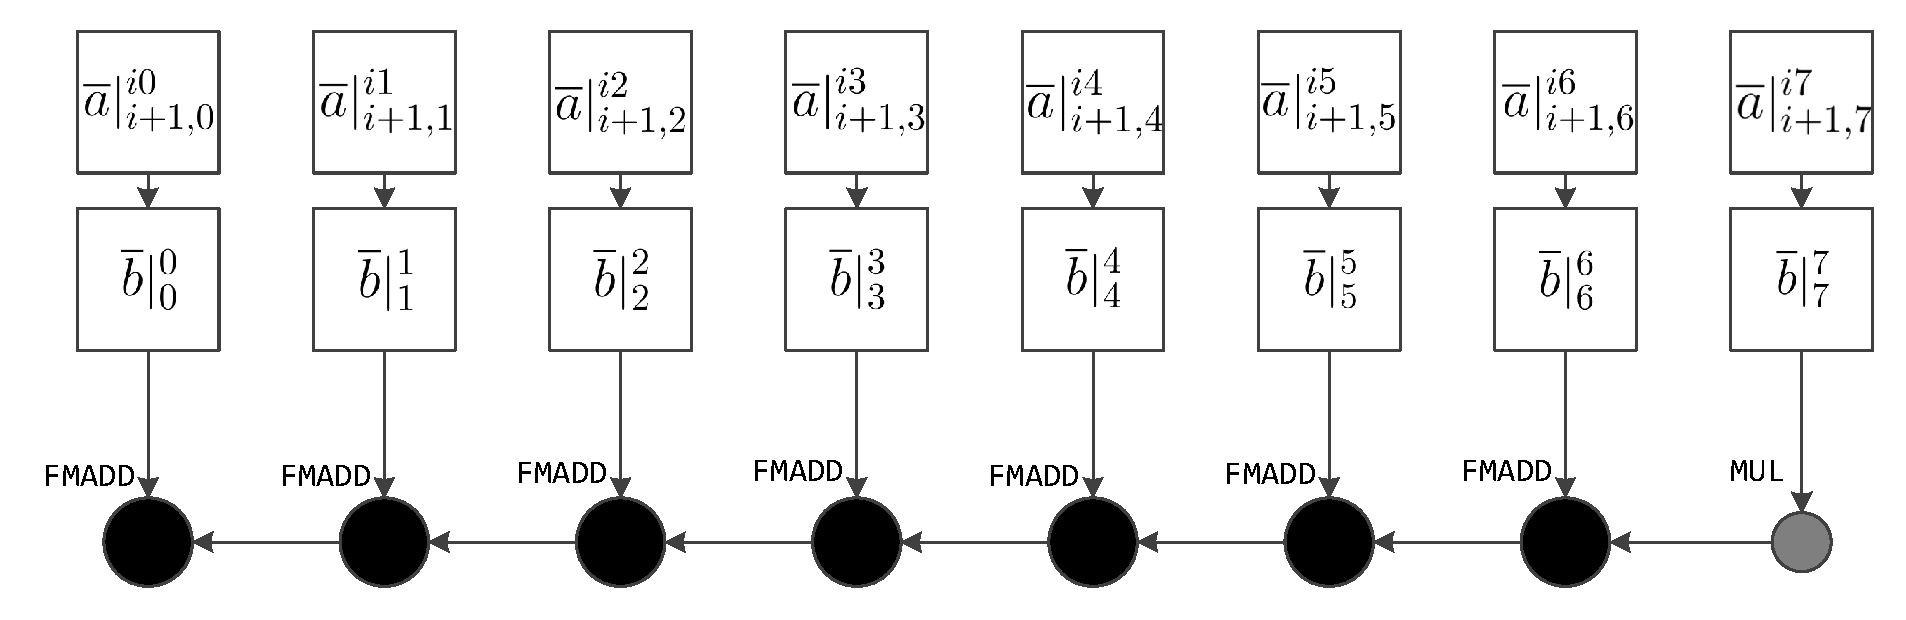
\includegraphics[width=1.00\textwidth]{./fig/vec_spec_matrices_fmadd.pdf}
\singlespacing
\captionstyle{center}\caption{Схема вычисления двух соседних строк результирующей матрицы путем последовательного сложения попарно перемноженных векторов.}
\label{fig:text_4_spec_matr_fmadd}
\end{figure}

Для вычисления значения $\overline{r}|_{i + 1}^i$ потребуется 8 векторных операций (1 mul и 7 fmadd) (см. рис.~\ref{fig:text_4_spec_matr_fmadd}).

Рассмотрим функцию перемножения двух матриц размера $8 \times 8$, с помощью использования комбинированных операций.
Для реализации выполним полную загрузку обеих матриц $a$ и $b$.
Далее требуется сформировать 8 векторов вида $\overline{b}|_j^j$, для чего потребуется еще 8 операций perm (для каждой пары загруженных строк матрицы $b$ нужно выполнить дублирование первой строки и дублирование второй строки).

\begin{lstlisting}[caption={Векторизованная версия перемножения матриц $8 \times 8$.},label={lst:text_4_spec_matr_mul8x8_opt}]
void mul_8x8_opt(float* __restrict a, float* __b, float* __restrict r)
{
    ...
    ind_df = _mm512_set_epi32(7,6,5,4,3,2,1,0,7,6,5,4,3,2,1,0);
    ind_ds = _mm512_set_epi32(15,14,13,12,11,10,9,8,
                              15,14,13,12,11,10,9,8);
    ...
    b0 = LD(&b[0]);
    b1 = _mm512_permutexvar_ps(ind_ds, b0);
    b0 = _mm512_permutexvar_ps(ind_df, b0);
    ...
    b6 = LD(&b[6 * V8]);
    b7 = _mm512_permutexvar_ps(ind_ds, b6);
    b6 = _mm512_permutexvar_ps(ind_df, b6);

    a0 = LD(&a[0]);
    ...
    a6 = LD(&a[6 * V8]);

    ind_0 = _mm512_set_epi32(8,8,8,8,8,8,8,8,0,0,0,0,0,0,0,0);
    ...
    ind_7 = _mm512_set_epi32(15,15,15,15,15,15,15,15,
                             7,7,7,7,7,7,7,7);

#define BLOCK(N, A)                           \
    ST(&r[N * V8],                            \
      FMADD(PERMXV(ind_0, A), b0,             \
        FMADD(PERMXV(ind_1, A), b1,           \
          FMADD(PERMXV(ind_2, A), b2,         \
            FMADD(PERMXV(ind_3, A), b3,       \
              FMADD(PERMXV(ind_4, A), b4,     \
                FMADD(PERMXV(ind_5, A), b5,   \
                  FMADD(PERMXV(ind_6, A), b6, \
                    MUL(PERMXV(ind_7, A), b7)))))))));

    BLOCK(0, a0);
    BLOCK(2, a2);
    BLOCK(4, a4);
    BLOCK(6, a6);
}
\end{lstlisting}

После подготовки всех необходимых данных выполняется вычисление значений результирующей матрицы.
Блок операций \texttt{BLOCK} осуществляет вычисление двух соседних строк результирующей матрицы.
Реализация блока состоит из 8 операций perm, 1 операции mul и 7 операций fmadd, кроме того выполняется одна операция записи в память.
Всего выполняется четыре таких блока, что в сумме и с учетом операций подготовки данных приводит к следующему итогу: 8 простых операций чтения из памяти, 40 операций perm, 4 операции mul, 28 операций fmadd, 4 простые операции записи в память.
Итоговый код (без отображения некоторых повторяющихся участков) приведен на листинге~\ref{lst:text_4_spec_matr_mul8x8_opt} (полные коды доступны в \cite{iparGithub}).

Заметим, что 28 векторных операций fmadd и 4 векторные операции mul соответствуют $(28 \times 2 + 4) \times 16 = 960$ скалярным операциям, что в точности совпадает с количеством скалярных операций, требуемых для выполнения перемножения двух матриц размера $8 \times 8$.
Таким образом, в реализации нет лишних арифметических операций, и результат каждой выполненной операции влияет на конечный результат.

При реализации перемножения матриц размера $7 \times 7$, $6 \times 6$, $5 \times 5$ удаляются заведомо лишние векторные операции (например, умножение на вектор, все элементы которого равны нулю), однако все равно остаются элементы векторов, обработка которых избыточна, что приводит к снижению эффективности векторизации в этих случаях.
Приведем таблицу с точным подсчетом количества скалярных операций для невекторизованных функций и количества векторных операций для их векторизованных аналогов (см. таблицу~\ref{tbl:text_4_spec_matr_tabl}).

\begin{table}
\centering
\singlespacing
\captionstyle{center}\caption{Статистика по количеству операций в невекторизованном и векторизованном вариантах функций перемножения матриц размера $8 \times 8$, $7 \times 7$, $6 \times 6$, $5 \times 5$.}
\bigskip
\label{tbl:text_4_spec_matr_tabl}
\begin{tabular}{ | c | c | c | }
  \hline
  \ & Невекторизованный вариант & Векторизованный вариант \\ \hline\hline
  $8 \times 8$ & \makecell{512 mul, 448 add \\ 960 арифметических операций} & \makecell{4 mul, 28 fmadd, 40 perm \\ 960 арифметических операций} \\ \hline
  $7 \times 7$ & \makecell{343 mul, 294 add \\ 637 арифметических операций} & \makecell{4 mul, 24 fmadd, 35 perm \\ 832 арифметические операции} \\ \hline
  $6 \times 6$ & \makecell{216 mul, 180 add \\ 396 арифметических операций} & \makecell{3 mul, 15 fmadd, 24 perm \\ 528 арифметических операций} \\ \hline
  $5 \times 5$ & \makecell{125 mul, 100 add \\ 225 арифметических операций} & \makecell{3 mul, 12 fmadd, 20 perm \\ 432 арифметические операции}
 \\ \hline
\end{tabular}
\end{table}

Из таблицы~\ref{tbl:text_4_spec_matr_tabl} видно, что с уменьшением размера перемножаемых матриц возрастает избыточность вычислений (для размера $5 \times 5$ эта избыточность почти достигает двукратного размера), что сказывается отрицательно на эффективности векторизации.

\begin{figure}[ht]
\centering
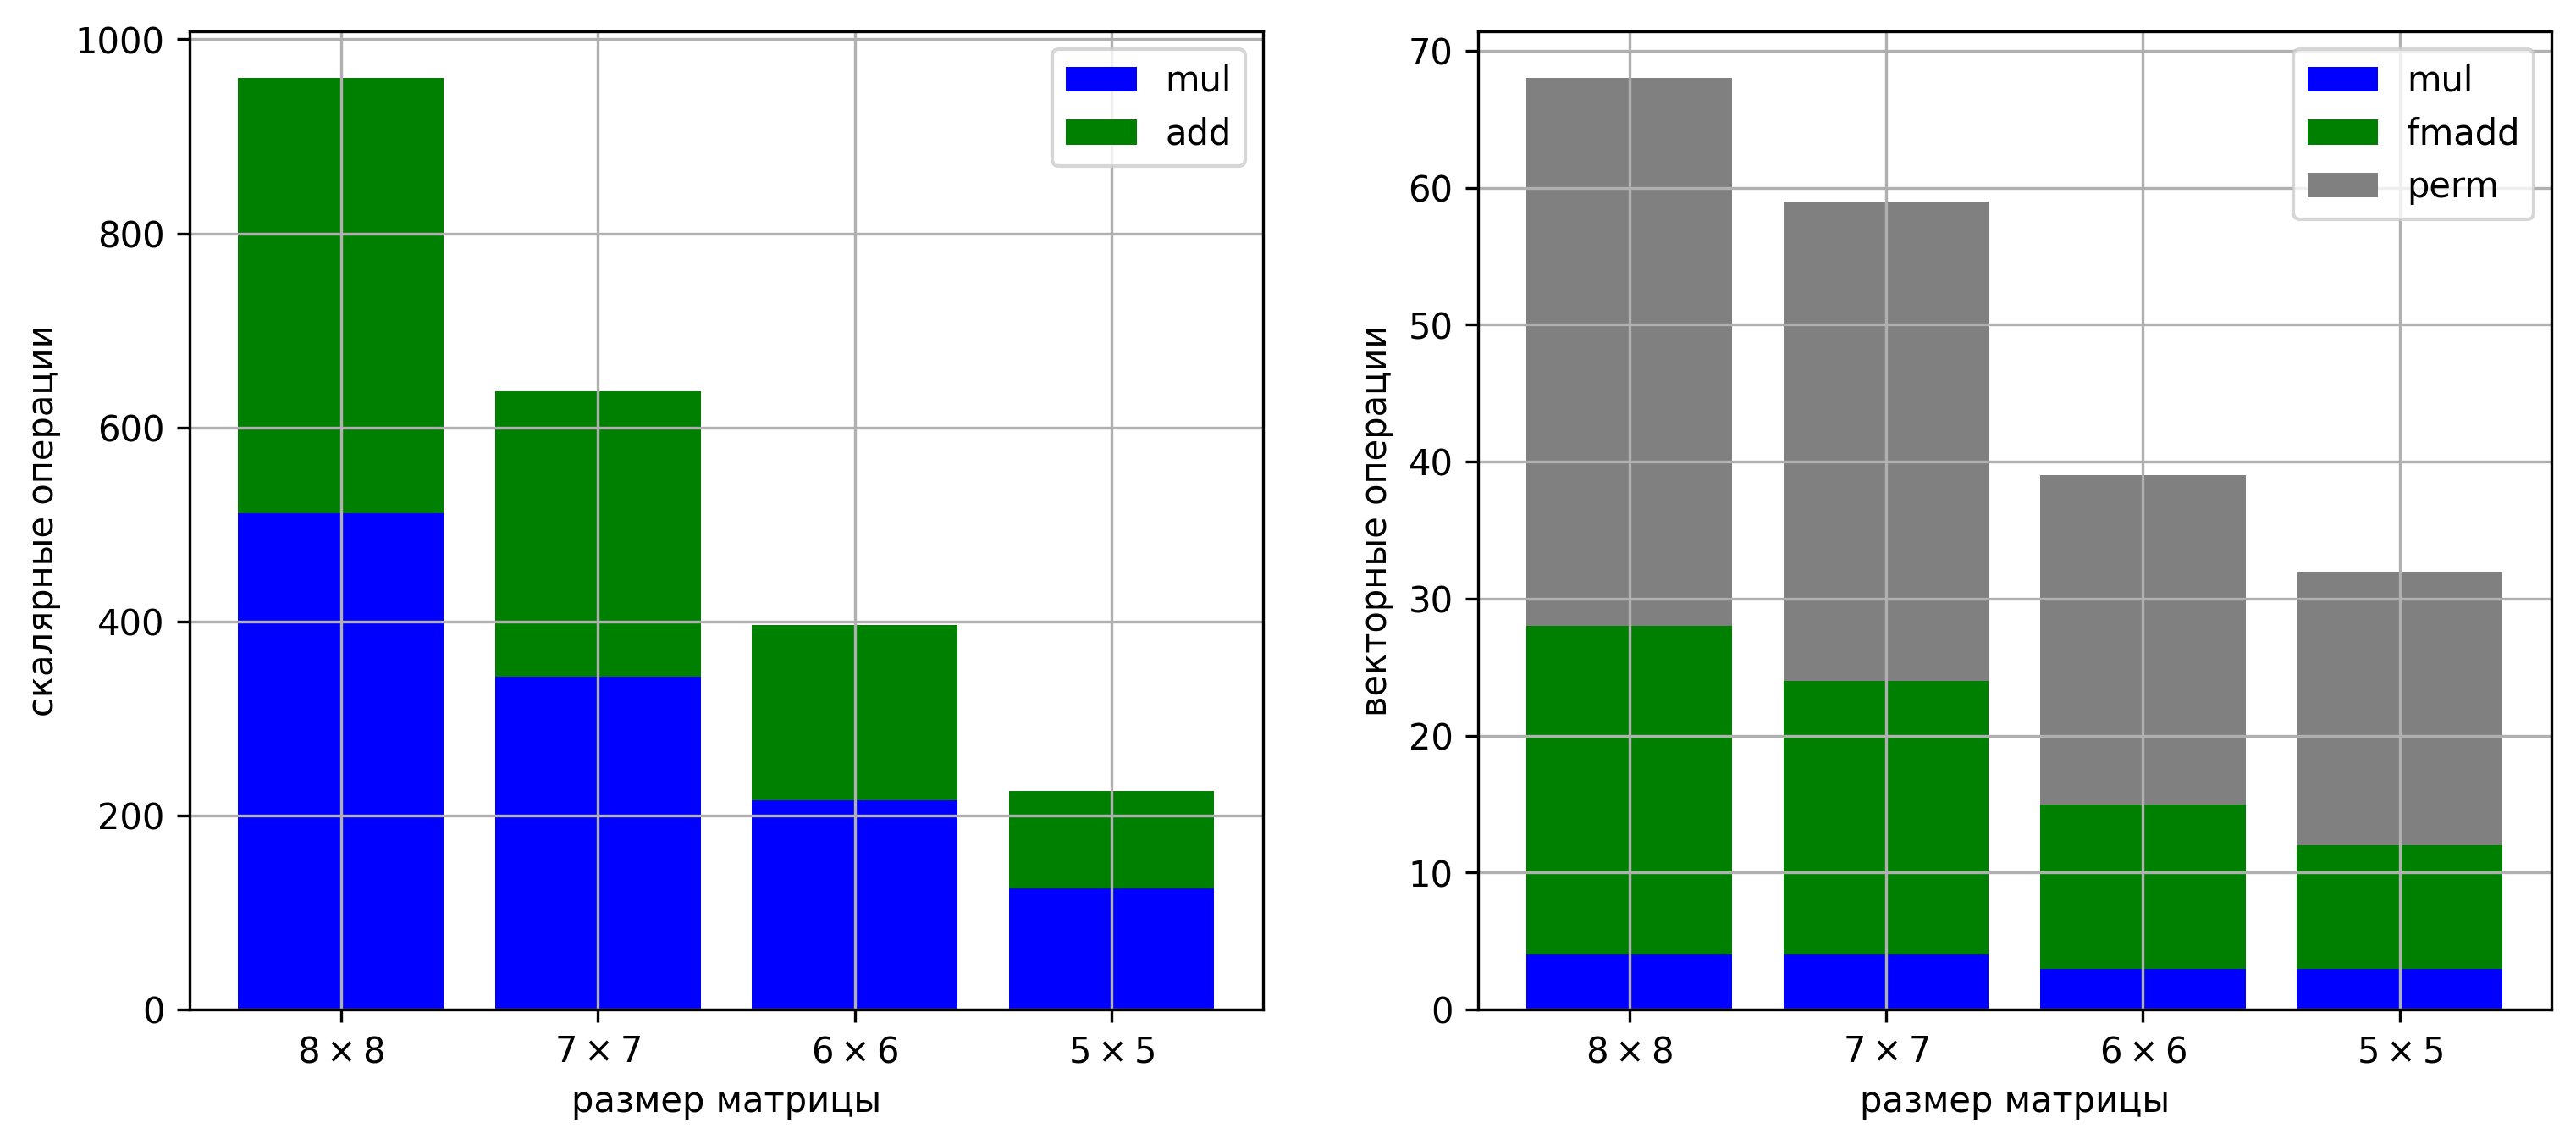
\includegraphics[width=1.00\textwidth]{./fig/vec_spec_matrices_stat.png}
\singlespacing
\captionstyle{center}\caption{Количество операций в скалярных и векторных вариантах перемножения матриц разных размеров.}
\label{fig:text_4_spec_matr_stat}
\end{figure}

На рис.~\ref{fig:text_4_spec_matr_stat} приведена статистика по количеству операций mul и add в скалярных версиях перемножения матриц, а также mul, fmadd и perm в векторизованных версиях.

Приведенный способ векторизации перемножения матриц размера был опробован на процессоре Intel Xeon Phi KNL.
Были рассмотрены 4 функции: \texttt{mul\_8x8}, \texttt{mul\_7x7}, \texttt{mul\_6x6}, \texttt{mul\_5x5}, выполняющие перемножение матриц соответствующих размеров.
Для каждой функции были рассмотрены 3 варианта реализации.
В качестве первого варианта был использован способ векторизации с параллельным вычислением сумм элементов векторов, описанный в разделе \ref{sec:text_4_small_matr_realization} (обозначен \texttt{VECT\_OLD}).
Для этого метода была применена оптимизация для сокращения количества операций по обращению в память.
В качестве второго варианта было взято прямое ручное вычисление каждого элемента результирующей матрицы, в котором все циклы были удалены и для каждого элемента путем многократного копирования был написан скалярный код (обозначен \texttt{FULL\_UNROLL}), в качестве третьего варианта взят рассмотренный подход, основанный на обращениях только к строкам матриц и использовании комбинированных операций fmadd (обозначен \texttt{VECT\_NEW}).

\begin{figure}[ht]
\centering
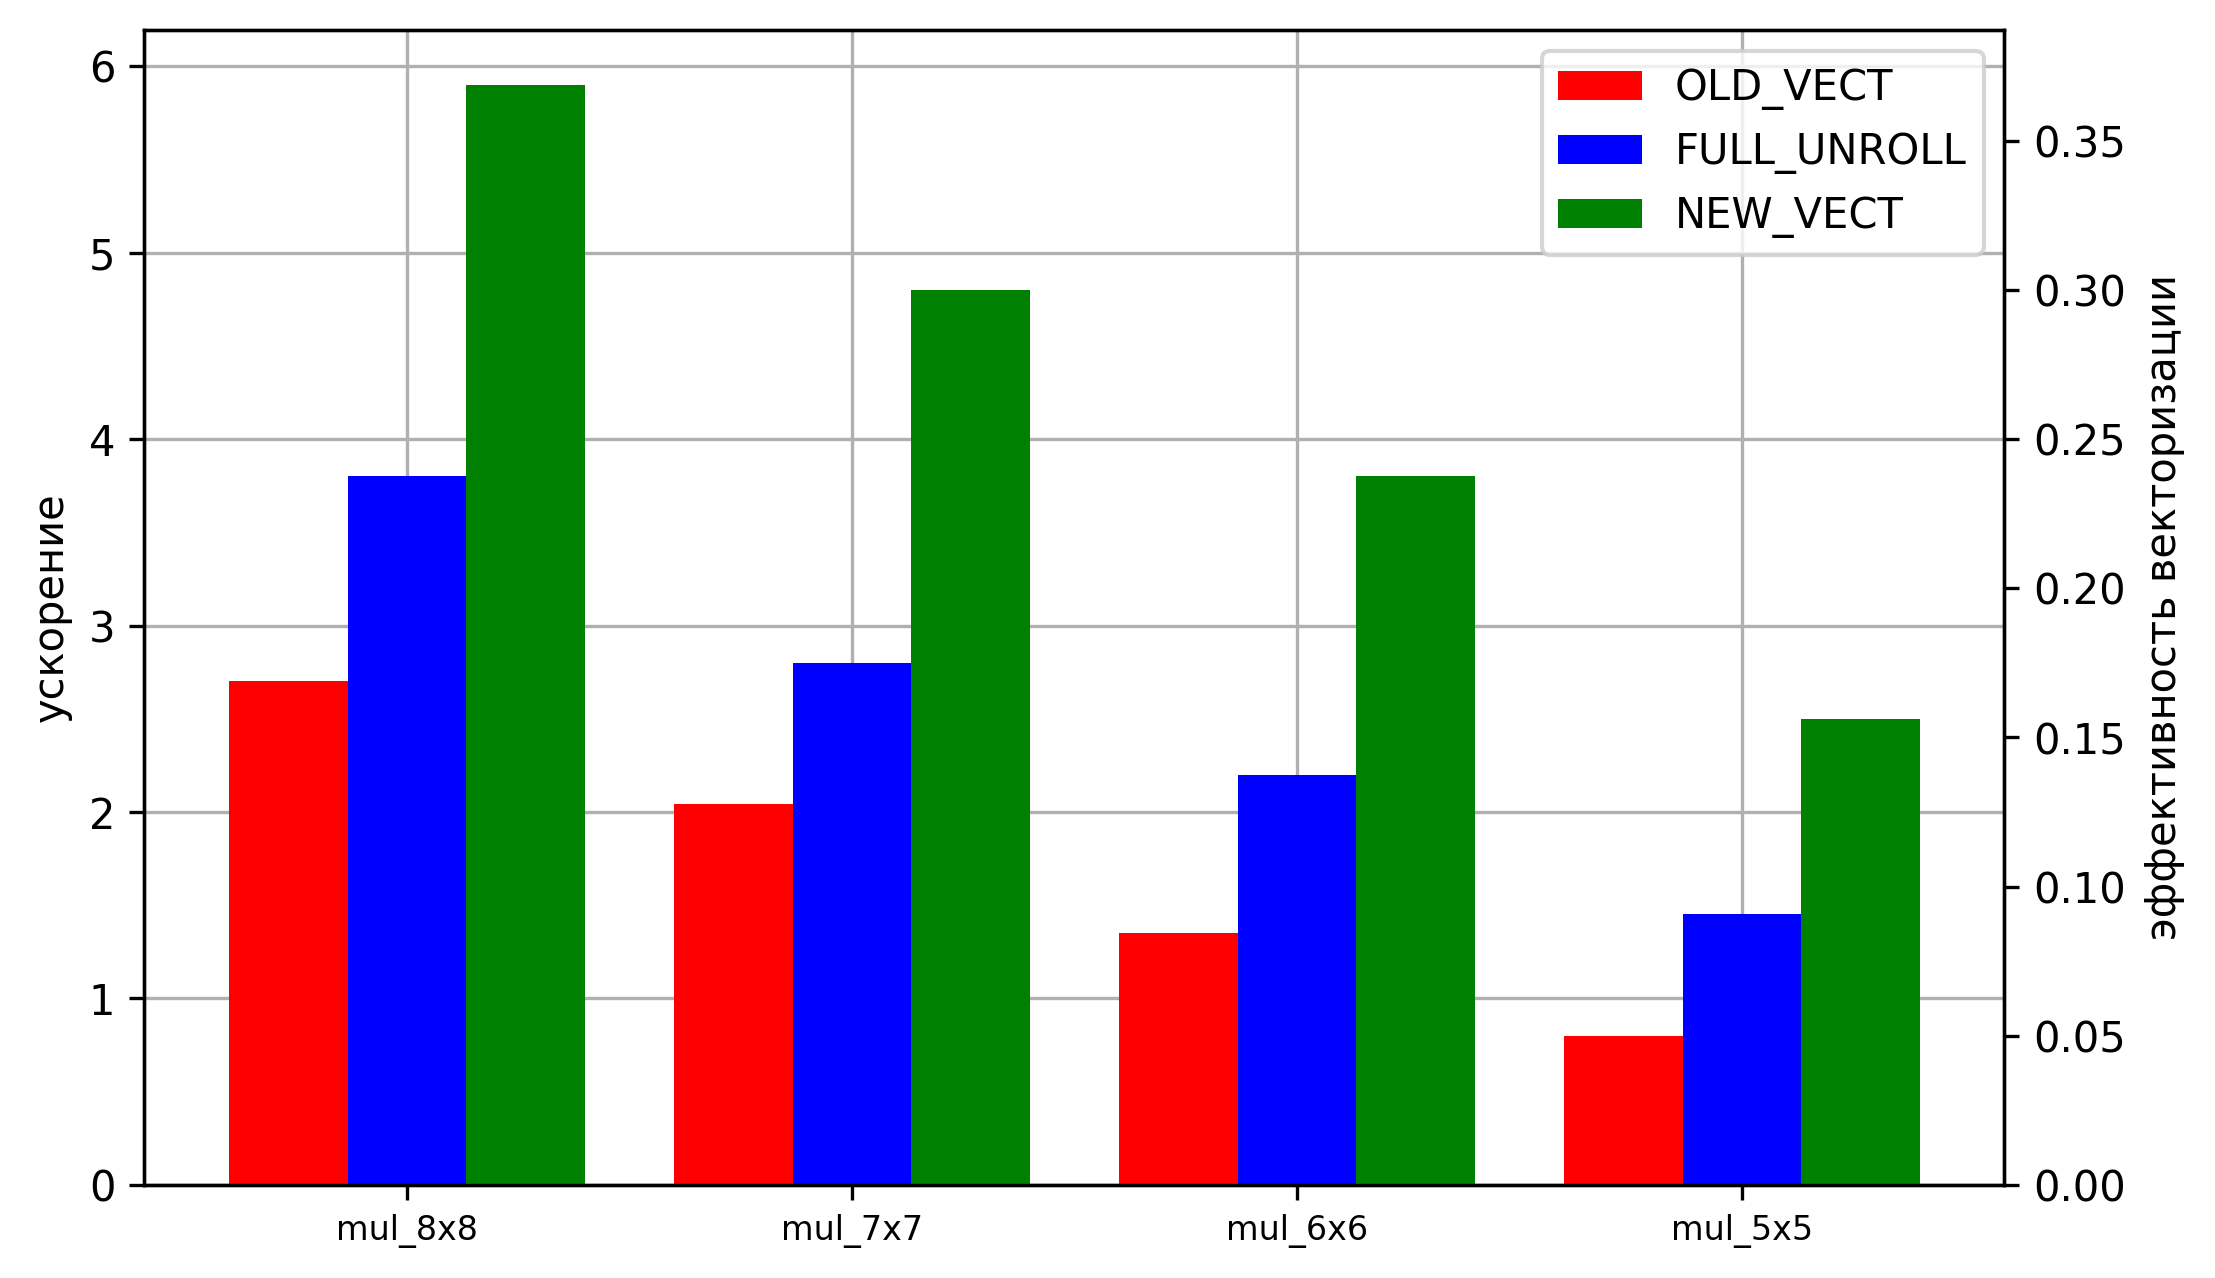
\includegraphics[width=0.6\textwidth]{./fig/vec_spec_matrices_res.png}
\singlespacing
\captionstyle{center}\caption{Ускорение и эффективность векторизации перемножения матриц с помощью подходов \texttt{OLD\_VECT}, \texttt{FULL\_UNROLL}, \texttt{NEW\_VECT}.}
\label{fig:text_4_spec_matr_res}
\end{figure}

На рис.~\ref{fig:text_4_spec_matr_res} показаны результаты тестирования описанных подходов на машине.
Из рисунка следует, что \texttt{OLD\_VECT} оказался наименее эффективным подходом, его применение даже менее выгодно, чем прямое написание скалярного кода.
Для матриц размера $5 \times 5$ этот метод оптимизации вовсе приводит к замедлению оригинальной неоптимизированной версии функции.
Метод \texttt{NEW\_VECT} демонстрирует наилучшие результаты из описанных подходов, на матрицах размера $8 \times 8$ продемонстрировано ускорение почти в 6 раз по сравнению с оригинальным кодом.
При понижении размерности матриц эффективность векторизации несколько снижается, однако даже для матриц размера $5 \times 5$ наблюдается ускорение примерно в 2,5 раза.

%---------------------------------------------------------------------------------------------------
% 5.3 - плоский цикл

% Плоский цикл.
\subsection{Плоский цикл}\label{sec:text_4_flat}

В разделе~\ref{sec:text_4_small_matr} были рассмотрены различные варианты векторизации функций, реализующих работу с малоразмерными матрицами и матрицами специального вида.
Эти варианты базировались на основной идее выделения однотипных операций замены их на векторные аналоги.
Из результатов, представленных в разделе~\ref{sec:text_4_small_matr}, можно заключить, что эффективность векторизации сильно зависит от способа выделения таких однотипных операций, от порядка обращения в память за данными, от избыточности вычислений и других факторов.

Неоднозначность и искусственность векторизации программного кода путем поиска однотипных операций порождает потребность выработки некоторого универсального подхода к векторизации, который мог бы применяться к широкому спектру расчетных приложений.

Исследования, описанные в этом разделе, направлены на определение и описание свойств программного контекста, векторизация которого может быть выполнена достаточно прозрачно, а результирующий код будет обладать высокой степенью эффективности.

\subsubsection{Понятие плоского цикла}

Векторизация программного контекста не может быть применена автоматически к коду произвольного вида.
В этом разделе определим подходящий для векторизации программный контекст специального вида -- плоский цикл -- и опишем его свойства \cite{Shabanov2021VecCFG}.

\begin{figure}[ht]
\centering
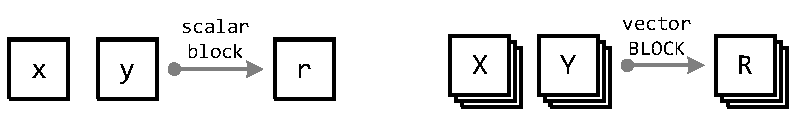
\includegraphics[width=0.8\textwidth]{./fig/vec_block_BLOCK.pdf}
\singlespacing
\captionstyle{center}\caption{Скалярный блок block и аналогичный ему \\ векторный блок BLOCK.}
\label{fig:text_4_vec_flat_fun_FUN}
\end{figure}

Идея плоского цикла состоит в объединении $w$ экземпляров скалярного блока в единый векторный блок, состоящий из аналогичных векторных инструкций.
На рис.~\ref{fig:text_4_vec_flat_fun_FUN} слева представлена схема скалярного блока \texttt{block}, со скалярными входными данными $x$ и $y$ и скалярным результатом $r$.
Будем считать, что этот блок соответствует концепции чистых вычислений, то есть результат его выполнения зависит только от значений $x$ и $y$ (например, отсутствуют побочные эффекты через глобальную память или операции ввода-вывода).
Идеология чистых вычислений берет свое начало из парадигмы функционального программирования \cite{Armstrong2013VecErlang}, использование такого подхода открывает возможности для оптимизации программного кода, в частности для компиляторов.
Если рассмотреть вместо одной копии скалярного блока \texttt{block} несколько копий ($w$ штук) с разными наборами входных данных, то их можно трактовать как выполнение векторного блока \texttt{BLOCK}, входными данными которого являются векторы $X$ и $Y$ длины $w$, а выходным значением является вектор $R$ также длины $w$.
В этом случае можно говорить, что векторный блок \texttt{BLOCK} представляет собой векторизованную версию скалярного блока \texttt{block} при ширине векторизации $w$ (рис.~\ref{fig:text_4_vec_flat_fun_FUN} справа).
В этом случае семантику векторного блока \texttt{BLOCK} можно записать в виде, представленном на листинге~\ref{lst:text_4_vec_flat_FUN_sem}.

\begin{singlespace}
\begin{lstlisting}[caption={Семантика векторного блока \texttt{BLOCK} -- векторизованной версии скалярного блока \texttt{block}.},label={lst:text_4_vec_flat_FUN_sem}]
// BLOCK
for (int i = 0; i < w; ++i)
{
   	r[i] = block(x[i], y[i])
}
\end{lstlisting}
\end{singlespace}

Цикл вида, представленного на в листинге~\ref{lst:text_4_vec_flat_FUN_sem}, будем называть плоским циклом.
Определим свойства, присущие плоскому циклу.

Прежде всего условимся считать, что плоский цикл это цикл for, индуктивная переменная которого меняется от $0$ до $w - 1$ (\texttt{for (int i = 0; i < w; ++i}).
Такое условие не является строгим ограничением, так как произвольный цикл for с количеством итераций $n$ может быть разбит (с помощью расщепления цикла по индуктивной переменной) на $\left\lfloor \frac{n}{w} \right\rfloor$ циклов с количеством итераций $w$ каждый, а также одного цикла с количеством итераций $n - \left\lfloor \frac{n}{w} \right\rfloor w$ (если $w \nmid n$), называемого эпилогом цикла.
Будем считать, что мы рассматриваем циклы с большим числом итераций $n \gg 1$.
В таком случае эпилогом цикла можно пренебречь, поэтому будем считать, что $w \mid n$, и эпилог отсутствует.

Во-вторых, будем считать, что внутри плоского цикла на $i$-ой итерации все обращения в память на запись имеют вид \texttt{a[i]}.
Обращения к глобальным данным на чтение могут иметь вид \texttt{a[i]} либо могут быть обращениями к глобальным скалярным данным.
Такое ограничение гарантирует отсутствие конфликтов между итерациями по обращениям в память.
Дополнительно будем считать, что при обращении в память все данные выровнены правильным образом, то есть адрес элемента \texttt{a[0]} выровнен в памяти на размер вектора.

Последним требованием будем считать отсутствие других межитерационных зависимостей внутри цикла.
Пример цикла с межитерационными зависимостями (обращение к глобальной переменной $s$), можно увидеть на листинге~\ref{lst:text_4_vec_not_flat}.

\begin{lstlisting}[caption={Пример цикла с межитерационной зависимостью.},label={lst:text_4_vec_not_flat}]
for (int i = 0; i < w; ++i)
{
   	s += x[i];
}
\end{lstlisting}

\begin{definition}
Плоским циклом будем называть цикл for, в котором индуктивная переменная $i$ последовательно принимает значения от $0$, до $w - 1$, где $w$ -- ширина векторизации (\texttt{for (int i = 0; i < w; ++i)}), и удовлетворяющий требованиям по обращению к глобальным данным (на $i$-ой итерации все обращения к данным на запись имеют вид \texttt{a[i]}, а обращения к данным на чтение имеют вид либо \texttt{a[i]}, либо являются чтением скаляров), выравниванию глобальных данных в памяти (все массивы данных, обращение к которым на $i$-ой итерации имеет вид \texttt{a[i]}, выровнены в памяти на размер вектора), а также отсутствию других межитерационных зависимостей.
\end{definition}

\begin{definition}
Цикл \texttt{for (int i = 0; i < w; ++i)}, в котором нарушаются некоторые требования, предъявляемые к плоским циклам, будем называеть квазиплоским.
\end{definition}

Учитывая все требования, предъявляемые к плоскому циклу, можно заключить, что итерации плоского цикла являются независимыми между собой, а значит могут выполняться в произвольном порядке, в том числе и одновременно.

Плоские циклы, обладающие описанными свойствами, представляют собой удобный контекст для векторизации, и в большинстве случаев они могут быть векторизованы с помощью векторных инструкций AVX-512\label{abbr:avx-8} с помощью перевода тела цикла в предикатное представление и замены скалярных инструкций векторными аналогами, реализованными с помощью функций-интринсиков \cite{IntelIntrinsicsGuide,Savin2020VecFlat}.
Таким образом, плоский цикл зачастую может быть заменем на векторный блок (или на несколько соседних векторных блоков в случае произвольного количества итераций $n > w$).

Многие практические вычислительные задачи состоят из выполнения однотипных вычислений, применяемых к разным наборам данных, которые можно сгруппировать, трансформировав в плоский цикл, как это продемонстрировано на рис.~\ref{fig:text_4_vec_flat_fun_FUN} на примере скалярного блока \texttt{block}.

Сложность векторизации тела полученного плоского цикла зависит от особенностей исходного блока \texttt{block}.
Чем сложнее управление внутри тела векторизуемого плоского цикла, тем больше трудностей может возникнуть в процессе выполнения векторизации.
Граф потока управления цикла используется для оценки анализа возможности векторизации этого цикла.

\subsubsection{Представление структуры тела плоского цикла в виде графа потока управления}

Граф потока управления (control flow graph, CFG)\label{abbr:cfg-1} является одним из видов промежуточного представления программы, которые используются в частности для выполнения оптимизаций исполняемого кода \cite{Muchnick1997Compilers}.
Узлами этого графа являются линейные участки, состоящие из последовательностей инструкций, а ребрами -- передача управления между этими линейными участками \cite{Rybakov2013CGF}.
Граф потока управления является логической структурой, отражающей параллелизм программы на уровне линейных участков.
Он активно используется компилятором для применения различных глобальных оптимизаций \cite{Aho2006Compilers}.

Кроме самой структуры графа потока управления для оптимизации программного кода важна статистическая информация об исполнении программы: количество выполнений различных линейных участков и данные о частоте переходов между ними.
Такая статистическая информация называется профилем исполнения, и для корректного проведения оптимизаций требуется правильным образом собирать и корректировать этот профиль \cite{Chetverina2015Profile}.
Для векторизации программного кода профиль исполнения программы приобретает особенную важность, так как на эффективность векторизации сильно влияет плотность и даже структура векторных масок, которая сильно разнится при сравнении результатов, полученных при генерации случайных входных данных, и при использовании данных реальных расчетов.

\begin{definition}
Плотностью векторной маски будем называть отношение количества единичных битов в ней к ее длине.
\end{definition}

\begin{figure}[ht]
\centering
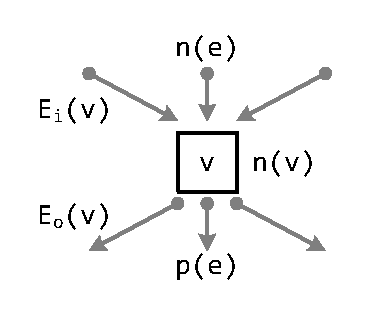
\includegraphics[width=0.4\textwidth]{./fig/vec_cfg.pdf}
\singlespacing
\captionstyle{center}\caption{Узел CFG с входящими и выходящими ребрами.}
\label{fig:text_4_vec_flat_cfg}
\end{figure}

В качестве профиля исполнения приложения будем использовать данные, содержащие только счетчики узлов и ребер, а также вероятности ребер.
Обозначим некоторый узел CFG через $v$.
Пусть в него входят несколько ребер, а также выходят несколько ребер (рис.~\ref{fig:text_4_vec_flat_cfg}).

\begin{definition}
Счетчиком ребра $e$ будем называть количество переходов по этому ребру в процессе выполнения программы.
Значение счетчика ребра будем обозначать $n(e)$.
\end{definition}

\begin{definition}
Счетчиком узла $v$ будем называть суммарное количество счетчиков всех входных ребер либо всех выходных ребер (для внутренних узлов CFG эти значения совпадают).
\begin{equation}
	n(v) = \sum_{e \in E_i(v)}{n(e)} = \sum_{e \in E_o(v)}{n(e)}
\end{equation}
\end{definition}

\begin{definition}
Вероятностью ребра $e$ будем называть отношение счетчика этого ребра с счетчику узла, из которого это ребро выходит.
\begin{equation}
	\forall e \in E_o(v): p(e) = \frac{n(e)}{n(v)}
\end{equation}
\end{definition}

Построенный по телу плоского цикла граф потока управления с собранным профилем исполнения используется для принятия решения о выборе методов векторизации программного контекста.

\subsubsection{Семантика векторных инструкций AVX-512 с точки зрения плоского цикла}

Векторные инструкции AVX-512\label{abbr:avx-9} позволяют не просто объединять $w$ однотипных скалярнях операций, но также обеспечивают выборочное их исполнение с помощью векторных масок (предикатов), что делает инструкции AVX-512 мощным инструментом для векторизации плоских циклов.
В этом разделе опишем семантику некоторых векторных инструкций AVX-512, пригодных для векторизации плоских циклов.
При этом основное внимание будем уделять операциям, работающим с вещественными числами, так как обычно они являются основой высоконагруженных суперкомпьютерных приложений.
Все приводимые ниже векторные инструкции работают с упакованными данными формата float, для данных формата double в AVX-512 существуют аналогичные инструкции.

Условимся обозначать маленькими латинскими буквами элементы данных, с которыми мы оперируем в процессе счета (в рассматриваемом случае это вещественные элементы данных формата float).
Арифметические операции будем записывать в естественном виде, например $r = a + b$ означает вычисление суммы двух элементов данных.
Векторы, составленные из отдельных элементов будем записывать с помощью заглавных латинских букв.
То есть будем считать, что $A$ это вектор, состоящий из $w$ отдельных элементов $A[i]$.
Под записью $R = A + B$ будем понимать поэлементную сумму векторов $A$ и $B$ и копирование результата в вектор $R$.
Заменяя операцию сложения произвольной операцией $op$ (не обязательно операцией двух аргументов), получим запись семантики векторной поэлементной операции в виде $R = op \ A, B$.

Для рассмотрения семантики векторных операций, работающих с масками, нам понадобится представление векторных предикатов.
Предикаты будем обозначать латинскими буквами в галочкой наверху.
Использование предиката при выборе одного из двух аргументов будем записывать с помощью тернарного оператора.
Таким, образом в выражении $r = \check{p} \ ? \ a : b$ элемент $r$ принимает значение $a$ при истинном значении предиката $\check{p}$, в противном случае он принимает значение $b$.
В векторном аналоге этой записи $R = \check{P} \ ? \ A : B$ эта операция выполняется поэлементно для элементов векторов, находящихся в позиции $i$ ($0 \le i < w$).

После рассмотрения записи семантики векторных инструкций для векторизации плоских циклов рассмотрим основные классы пригодных для этого инструкций (примеры операций и их семантика приведены в таблице~\ref{tbl:text_4_flat_avx512semantic}.

\begin{table}
\centering
\singlespacing
\captionstyle{center}\caption{Инструкции AVX-512 для работы с вещественными числами \\ и их семантика.}
\bigskip
\label{tbl:text_4_flat_avx512semantic}
\begin{tabular}{ | c | c | }
  \hline
  Имя инструкции & Семантика инструкции \\ \hline\hline
  \makecell{VMOVAPS, VMOVUPS, VSQRTPS, \\ VGETEXPPS, VGETMANTPS, \\ VRCP14PS, VREDUCEPS, VRNDSCALEPS, \\ VRSQRT14PS, VSCALEFPS} & $\begin{matrix} R = op \ A \\ R = \check{P} \ ? \ (op \ A) : R \\ R = \check{P} \ ? \ (op \ A) : 0 \end{matrix}$ \\ \hline
  \makecell{VADDPS, VANDPS, VANDNPS, VDIVPS, \\ VMAXPS, VMINPS, VMULPS, VORPS, \\ VSUBPS, VRANGEPS} & $\begin{matrix} R = op \ A, B \\ R = \check{P} \ ? \ (op \ A, B) : R \\ R = \check{P} \ ? \ (op \ A, B) : 0 \end{matrix}$ \\ \hline
  \makecell{VFMADD*PS, VFMSUB*PS, \\ VFNMADD*PS, VFNMSUB*PS} & $\begin{matrix} R = op \ R, A, B \\ R = \check{P} \ ? \ (op \ R, A, B) : R \\ R = \check{P} \ ? \ (op \ R, A, B) : 0 \end{matrix}$ \\ \hline
  \makecell{VCMPPS} & $\begin{matrix} \check{P} = op \ A, B \\ \check{P} = \check{Q} \ ? \ (op \ A, B) : 0 \end{matrix}$ \\ \hline
  \makecell{VBLENDPS} & $\begin{matrix} R = \check{P} \ ? \ A : B \end{matrix}$ \\ \hline
\end{tabular}
\end{table}

Первым типом рассматриваемых операций являются векторные операции с одним аргументом.
В этом случае к каждому элементу вектора применяется одна и та же операция (например, получение обратной величины или вычисление квадратного корня), после чего результаты записываются в результирующий вектор.
С помощью дополнительного предикатного аргумента можно выбрать множество обрабатываемых элементов вектора.
Если же к элементу вектора не должна быть применена рассматриваемая операция, то соответствующий элемент результирующего вектора может быть либо оставлен без изменения, либо обнулен (это регулируется отдельным флагом в инструкции).

Аналогичным образом записывается семантика арифметических векторных инструкций с двумя и тремя аргументами.
Операции с двумя аргументами это обычные операции сложения, вычитания, умножения, получения максимума из двух чисел и другие.
Арифметические операции с тремя аргументами это так называемые сдвоенные, или комбинированные FMA\label{abbr:fma-3} операции, которые позволяют за одну операцию вычислитель значение $\pm a \cdot b \pm c$.

Следующий большой класс операций это операции сравнения.
В таблице этот класс представлен единственной операцией VCMPPS, однако данная операция скрывает в себе все множество различных операций сравнения (VCMPEQPS, VCMPLEPS, VCMPNEPS и остальные).
Эти операции выполняют поэлементное сравнение двух векторов и записывают результаты в векторный предикат.

Последний рассматриваемый класс векторных инструкций представлен одной инструкцией VBLENDPS, которая является реализацией векторного тернарного оператора $R = \check{P} \ ? \ A : B$.

На самом деле, глядя на таблицу~\ref{tbl:text_4_flat_avx512semantic}, можно заметить, что описания семантики всех приведенных в ней векторных операций являются просто плоскими циклами в явном виде.
Верно также и обратное -- если некий плоский цикл можно записать в виде семантики одной или нескольких векторных инструкций, то он может быть реализован с помощью этих инструкций.

% Векторизация метода погруженных границ - потери производительности при векторизаии неплоских циклов.
\subsubsection{Векторизация с помощью представления расчетов в виде композиции плоских циклов}\label{sec:text_4_ibm}

В том случае, если вычисления организованы таким образом, что они могут трактоваться как композиция плоских циклов, а тела этих плоских циклов являются достаточно простыми с точки зрения управления, оптимизирующий компилятор может успешно создавать векторизованный код.
В этом случае даже нет необходимости явно использовать ассемблерные вставки или функции-интринсики.
В этом разделе рассмотрим основные аспекты приведения программного кода в форму, пригодную для автоматической векторизации \cite{Rybakov2023VecIBM}.
Подходы, применяемые к векторизации плоских циклов, могут частично применяться также к квазиплоским циклам.
Такие циклы все равно могут быть векторизованы, однако это может приводить к потере производительности.
Также в этом разделе будет проведен анализ потерь производительности при векторизации квазиплоских циклов на примере газодинамических расчетов с использованием метода погруженных границ для расчета обтекания тела со сложной геометрией, реализация которого приведена в разделе~\ref{sec:text_1_immersed_boundary_method_realization}.

Для анализа эффективности векторизации проводился эксперимент по организации программного кода газодинамического решателя, работающего с данными в формате double (вещественные числа размера 64 бита) с целью векторизации под микропроцессоры Intel Xeon Phi KNL\label{abbr:knl-7}.
Тексты анализируемых в этом разделе программных кодов доступны в \cite{ibmGithub}.

\begin{lstlisting}[caption={Организация данных в виде <<массив структур>>.},label={lst:text_4_vec_ibm_list_of_struct}]
struct Cell
{
    double rho;
    double u; double v; double w;
    double p;
    double rho_u; double rho_v; double rho_w;
    double E;
};
Cell cells[N];

void d_to_u()
{
    for (int i = 0; i < N; i++)
    {
        double rho = cells[i].rho;
        double u = cells[i].u;
        double v = cells[i].v;
        double w = cells[i].w;
        double p = cells[i].p;

        cells[i].rho_u = rho * u;
        cells[i].rho_v = rho * v;
        cells[i].rho_w = rho * w;
        cells[i].E = 0.5 * rho * (u * u + v * v + w * w)
                     + p / (GAMMA - 1.0);
    }
}
\end{lstlisting}

Рассмотрим на примере реализации функции \texttt{d\_to\_u} из общей схемы вычислений, представленной на рис.~\ref{fig:text_4_ibm_immersed_boundary_method_cheme}, способы организации данных для эффективного проведения вычислений.
Итак, функция \texttt{d\_to\_u} переводит вектор величин $D = [\rho, u, v, w, p]$ в вектор величин $U = [\rho, \rho u, \rho v, \rho w, E]$ для каждой расчетной ячейки.
При этом все ячейки обрабатываются в цикле независимо друг от друга.
Интуитивным способом вычисления могут быть организованы в виде следующей схемы: для каждой ячейки создается структура, которая содержит все необходимые величины, и действия по переводу вектора $D$ в вектор $U$ выполняется над полями этой структуры (листинг~\ref{lst:text_4_vec_ibm_list_of_struct}).

При попытке векторизации цикла из листинга~\ref{lst:text_4_vec_ibm_list_of_struct} во время объединения $w$ итераций вместо чтения из памяти скалярного значения (например, плотности) должно происходить чтение значений плотности из несколько последовательно расположенных структур данных.
То есть чтение вектора плотностей должно осуществляться не из последовательной области памяти.
Для таких целей в наборе векторных инструкций AVX-512\label{abbr:avx-10} предусмотрены инструкции gather/scatter, однако их эффективность гораздо ниже чтения последовательной области памяти размера 512 бит даже при использовании предварительной подкачки данных.
И хоть организация данных виде <<массива структур>> наиболее предпочтительная с точки зрения идеологии объектно-ориентированного программирования, она оказывается непригодной для успешного применения векторизации.

\begin{lstlisting}[caption={Организация данных в виде <<набор массивов>>.},label={lst:text_4_vec_ibm_set_of_lists}]
double rhos[N];
double us[N]; double vs[N]; double ws[N];
double ps[N];
double rho_us[N]; double rho_vs[N]; double rho_ws[N];
double Es[N];

void d_to_u()
{
    for (int i = 0; i < N; i++)
    {
        double rho = rhos[i];
        double u = us[i];
        double v = vs[i];
        double w = ws[i];
        double p = ps[i];

        rho_us[i] = rho * u;
        rho_vs[i] = rho * v;
        rho_ws[i] = rho * w;
        Es[i] = 0.5 * rho * (u * u + v * v + w * w)
                + p / (GAMMA - 1.0);
     }
}
\end{lstlisting}

Естественным решением оптимизации вычислений является организация расположения данных в памяти в виде набора массивов (листинг~\ref{lst:text_4_vec_ibm_set_of_lists}).
Теперь после объединения нескольких итераций цикла команды скалярного доступа в память трансформируются в векторные аналоги доступа к последовательной области памяти размера 512 бит.
Вся же арифметика, которая присутствует в коде функции (операции сложения, вычитания, умножения, деления, взятие обратной величины) имеет свои векторные аналоги в наборе инструкций AVX-512.

Другой критической проблемой, влияющей на эффективность векторизации кода, является наличие условных операций внутри векторизуемого цикла.
Конечно набор инструкций AVX-512 содержит специальные масочные аргументы, с помощью которых можно векторизовать программный код с управлением практически любой сложности (разветвленное управление, гнезда циклов, циклы с вызовами функций), однако при увеличении количества условий в коде эффективность векторизации снижается.

\begin{lstlisting}[caption={Гнездо циклов с условием во внутреннем цикле.},label={lst:text_4_vec_ibm_nest}]
for (int k = 0; k < NZ; k++)
{
    for (int j = 0; j < NY; j++)
    {
        for (int i = 0; i < NX; i++)
        {
            if (i == 0)
            {
                // left boundary condition
                ...
            }

            // rest code
            ...
        }
    }
}
\end{lstlisting}

В качестве примера такого негативного эффекта можно рассмотреть логику гнезда циклов из функции \texttt{calc\_flows}, в которой корректируются газодинамические величины $U = [\rho, \rho u, \rho v, \rho w, E]$ с помощью потоков через все грани ячейки.
Если рассматриваемая расчетная область представлена структурированной сеткой размера $NX \times NY \times NZ$ по направлениям $i$, $j$, $k$ соответственно, то при учете потоков через левую грань каждой ячейки необходимо отдельно обрабатывать случай $i = 0$, что соответствует граничному условию расчетной области (см. листинг~\ref{lst:text_4_vec_ibm_nest}).
Аналогично нужно рассматривать особые случаи для всех шести граней ячейки, что резко увеличивает количество условий внутри цикла и снижает эффективность векторизации.

Можно заметить, что все три цикла гнезда (по индуктивным переменным $i$, $j$, $k$) не содержат межитерационных зависимостей, они могут быть переставлены местами, как и итерации внутри любого из них.
Также можно заметить, что условия обработки границ расчетной области не являются уникальными для тройки координат ячейки $(i, j, k)$, но являются константными для некоторого среза ячеек сетки.
Это означает, что для гнезда циклов такое условие является частично константным, и гнездо может быть разбито по этому условию (расщепление цикла по условию.
На листинге~\ref{lst:text_4_vec_split_nest} продемонстрировано разбиение гнезда циклов по условию $i = 0$, после чего итоговое гнездо, содержащее основную часть вычислений, освобождается от условия.
Аналогичным образом можно выполнить разбиение по остальным условиям, освободив от них основное гнездо циклов, которое после этого успешно векторизуется.

\begin{lstlisting}[caption={Расщепление гнезда циклов по условию.},label={lst:text_4_vec_split_nest}]
for (int k = 0; k < NZ; k++)
{
    for (int j = 0; j < NY; j++)
    {
        // left boundary condition with i = 0
        ...
    }
}

for (int k = 0; k < NZ; k++)
{
    for (int j = 0; j < NY; j++)
    {
        for (int i = 1; i < NX; i++)
        {
            // rest code
            ...
        }
    }
}
\end{lstlisting}

При таком расщеплении циклов по условию нарушается условие выровненности данных внутри цикла, то есть цикл становится квазиплоским.

На рис~\ref{fig:text_4_ibm_immersed_boundary_method_cheme} представлена общая схема выполнения расчетов для одной итерации численного метода.
Основными функциями в этих расчетах являются \texttt{approximate\_values}, \texttt{d\_to\_u}, \texttt{calc\_fgh}, \texttt{calc\_flows}, \texttt{u\_to\_d}.
Все эти функции содержат внутри себя обработку ячеек расчетной сетки в гнезде циклов либо в одном цикле.
Функция \texttt{approximate\_values} выполняет апроксимацию газодинамических величин в фиктивных ячейках, содержит векторные и матричные операции и сложное управление.
Функции \texttt{d\_to\_u}, \texttt{calc\_fgh}, \texttt{u\_to\_d} не содержат операторов передачи управления и при условии реорганизации данных в виде <<набор массивов>> могут быть представлены в виде композиции плоских циклов.
Функция \texttt{calc\_flows} с помощью расщепления гнезда циклов по 6 условиям может быть предствлена в виде композиции квазиплоских циклов.

Для автоматически векторизованного с помощью оптимизирующего компилятора icc программного кода расчета газодинамического потока с помощью схемы Стегера-Уорминга и метода погруженной границы был поставлен эксперимент по замеру ускорения и эффективности векторизации на микропроцессоре Intel Xeon Phi KNL.
Во время проведения эксперимента на модельной задаче был собран профиль исполнения до векторизации и после нее, результаты распределения времени исполнения между этими основными функциями представлены на рис.~\ref{fig:text_4_ibm_diagr}.

\begin{figure}[ht]
\centering
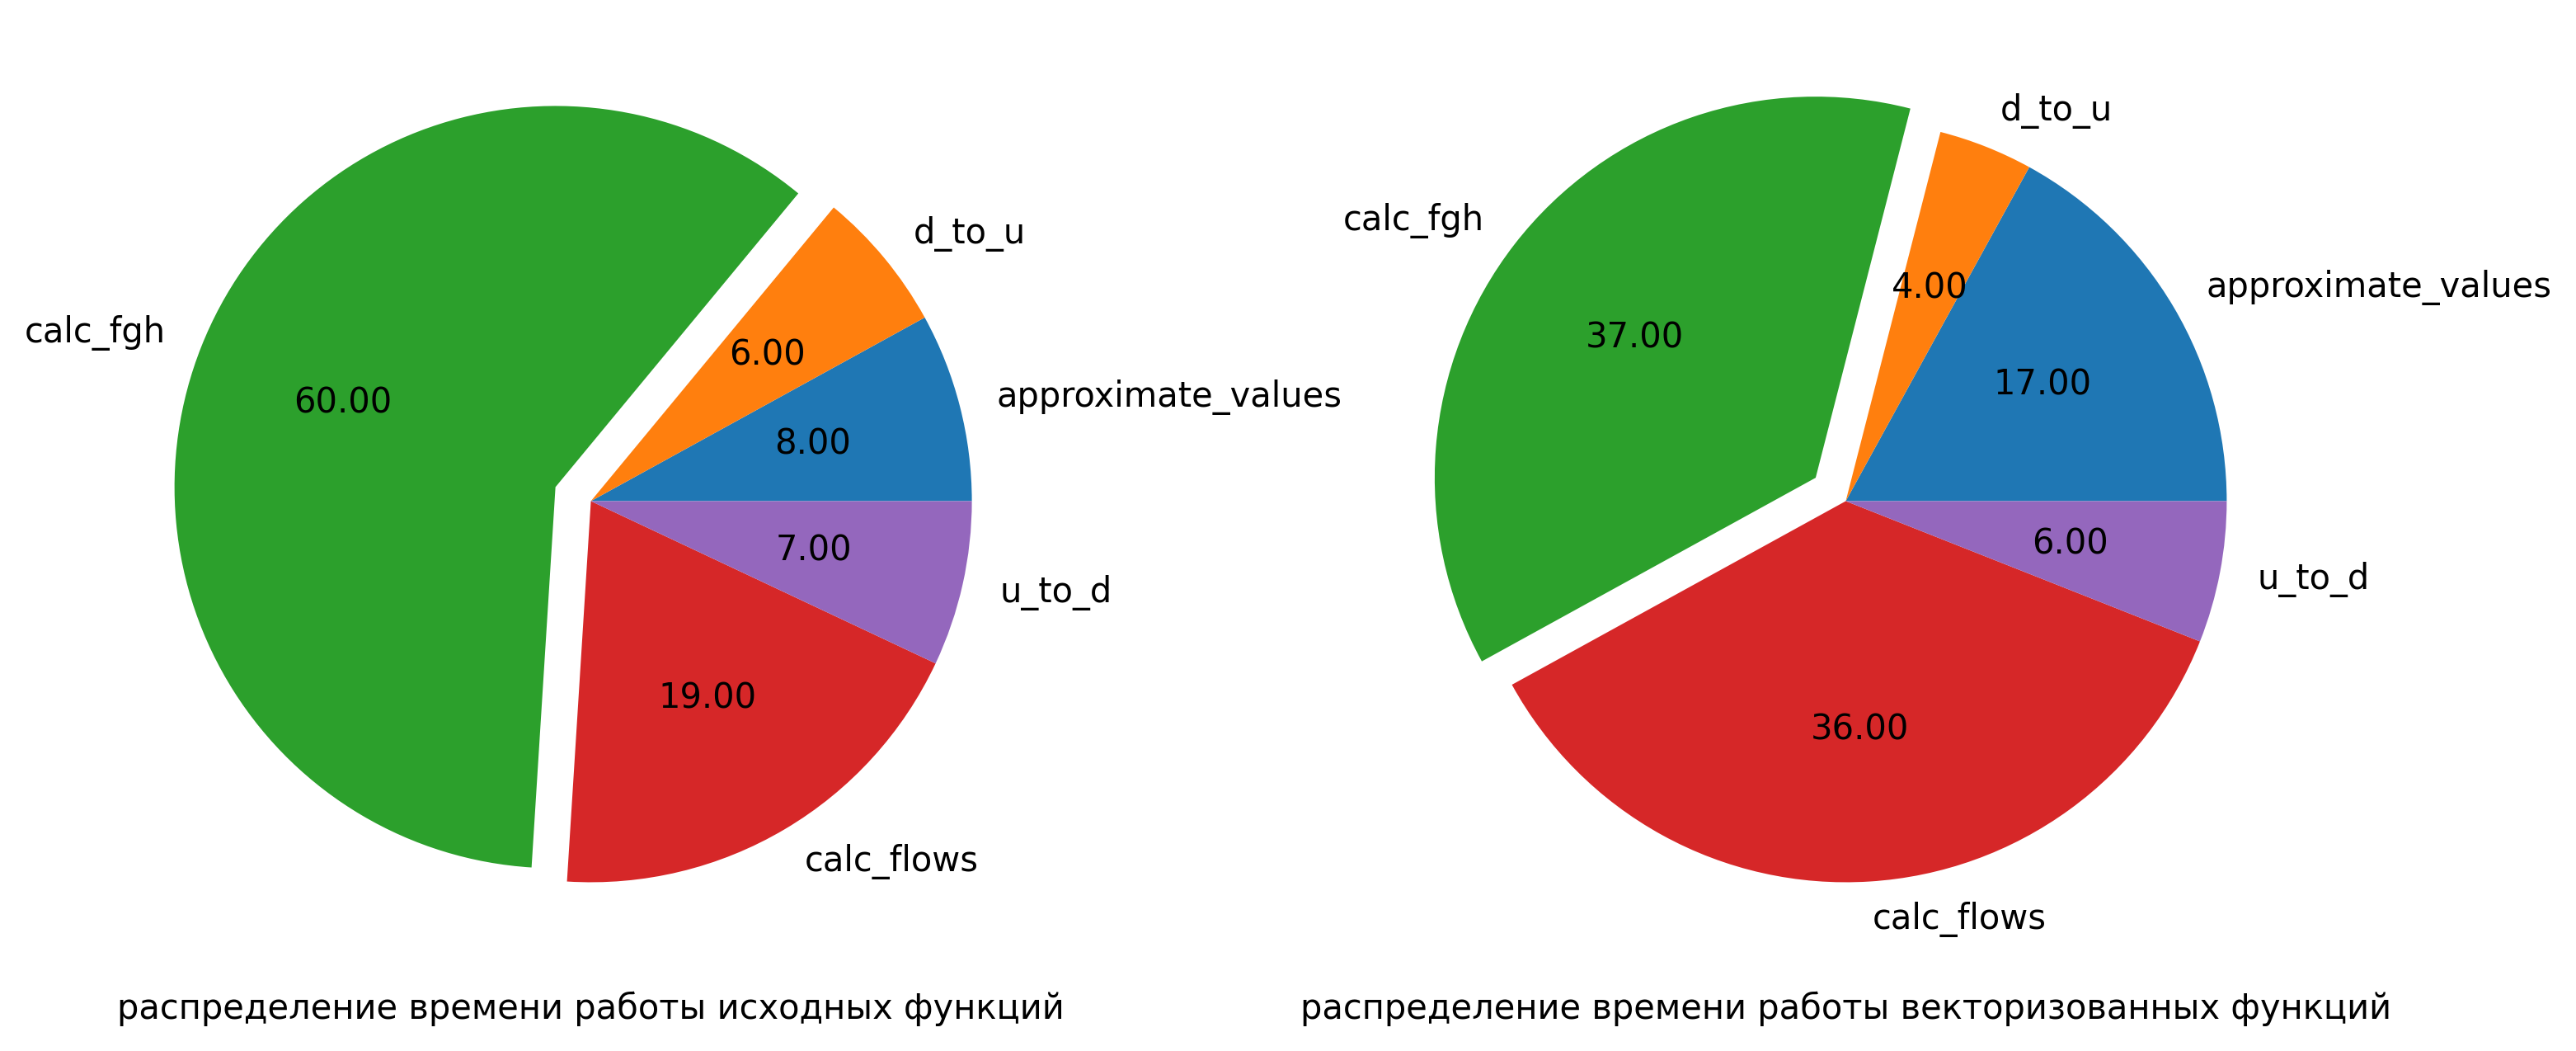
\includegraphics[width=1.0\textwidth]{./fig/vec_ibm_diagr.png}
\singlespacing
\captionstyle{center}\caption{Распределение времени выполнения отдельных функций газодинамического решателя.}
\label{fig:text_4_ibm_diagr}
\end{figure}

\begin{figure}[ht]
\centering
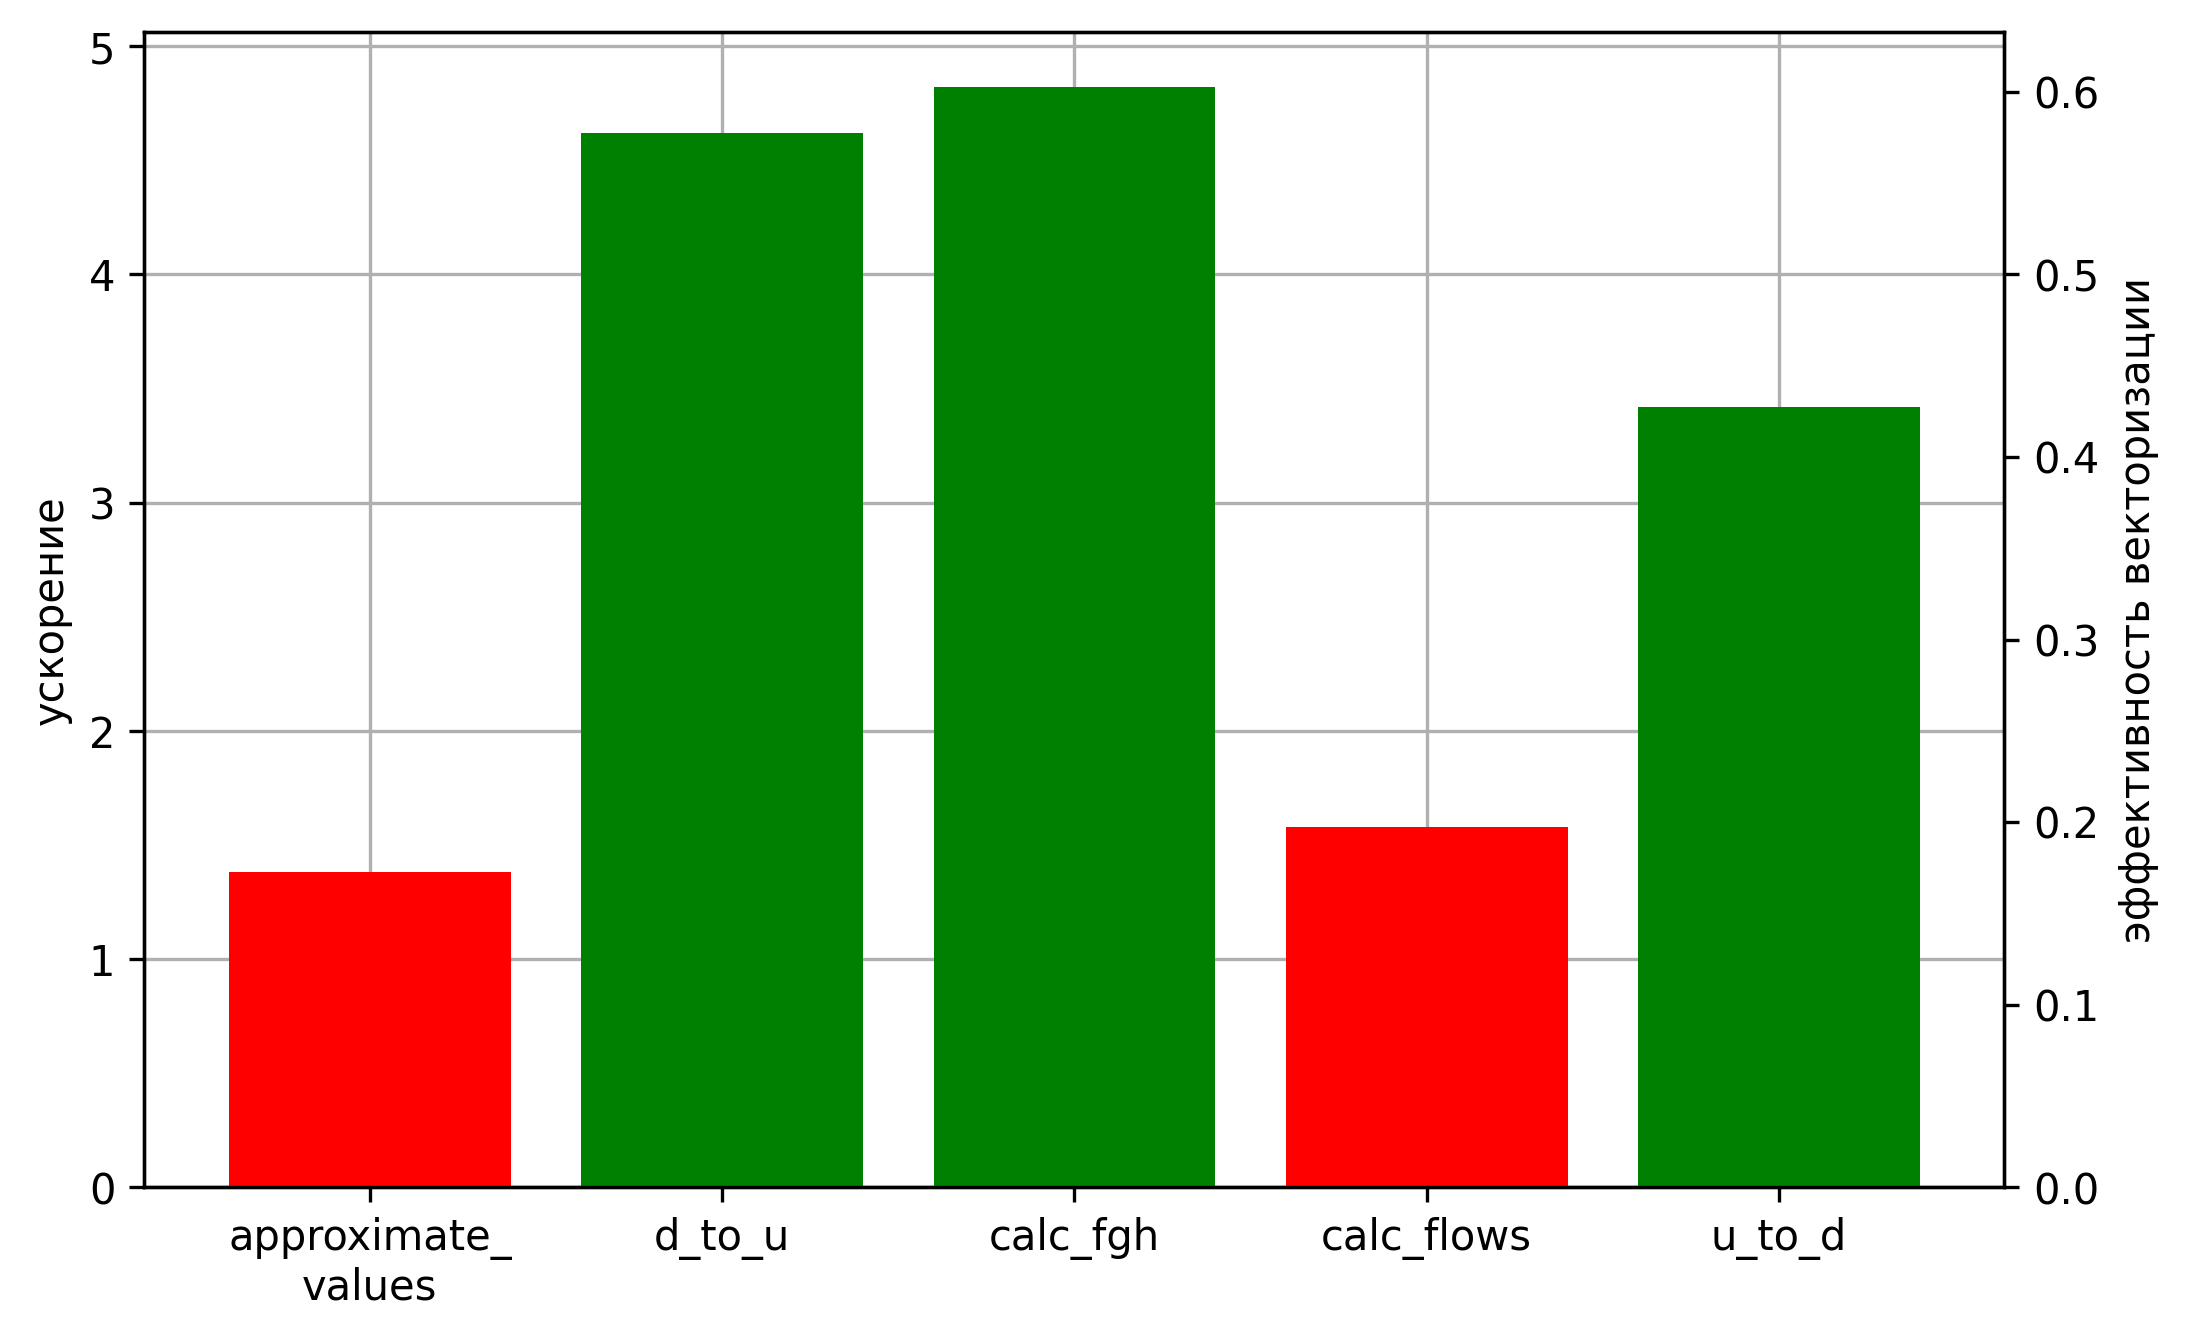
\includegraphics[width=0.6\textwidth]{./fig/vec_ibm_diagr2.png}
\singlespacing
\captionstyle{center}\caption{Ускорение кода и эффективность векторизации отдельных функций газодинамического решателя.}
\label{fig:text_4_ibm_diagr2}
\end{figure}

Также на рис.~\ref{fig:text_4_ibm_diagr2} представлены результаты ускорения и эффективности векторизации каждой функции.
Ускорение различных функций в результате векторизации сильно отличается друг от друга.
Причиной этому являются конкретные особенности каждой из этих функций.

Наибольшее ускорение продемонстрировала функция \texttt{calc\_fgh}, реализующая вычисление потоков $F^{\pm}$, $G^{\pm}$, $H^{\pm}$.
Этому способствовали следующие особенности этой функции.
Во-первых, функция содержит плоский цикл, полностью удовлетворяющий всем условиям, что делает возможным замену всех скалярных операций на векторные аналоги.
Во-вторых, в скалярной версии используются библиотечные вызовы \texttt{abs} (вычисление абсолютного значения) и \texttt{sqrt} (вычисление квадратного корня).
В наборе векторных инструкций AVX-512 есть векторные операции VAND (с помощью побитовой операцией над вещественным числом можно обратить в ноль бит знака этого числа), VSQRT, которые реализуют эти действия просто одной операцией, что сильно ускоряет исполнение.
Наконец, обилие операций умножения и сложения делает возможным применение векторных комбинированных операций вида $\pm a \cdot b \pm c$.

Также ускорение выше среднего продемонстрировали функции \texttt{d\_to\_u} и \texttt{u\_to\_d}.
Эти функции также состоят из плоских циклов, поэтому скалярные операции могут быть заменены на векторные аналоги.
Более низкое ускорение функции \texttt{u\_to\_d} объясняется наличием операций деления, которые выполняются медленнее операций сложения и умножения.

Показатель ускорения функции \texttt{calc\_flows} составил менее двух раз даже после избавления от всех условий, связанных с обработкой границ расчетной области.
Такая низкая эффективность векторизации объясняется тем, что внутри этой функции присутствуют циклы, которые не являются плоскими.
Так, например, в функции \texttt{calc\_flows} для корректировки консервативных величин внутри ячейки $(i, j, k)$ требуется обращаться за данными ко всем смежным по граням ячейкам: $(i \pm 1, j, k)$, $(i, j \pm 1, k)$, $(i, j, k \pm 1)$.
Это нарушает требование по унификации обращения к массивам данных на одной итерации плоского цикла и немедленно приводит к появлению операций gather/scatter, понижая эффективность векторизации.
Для функции \texttt{approximate\_values} ситуация выглядит аналогичной, так как для выполнения аппроксимации данных в ячейке $(i, j, k)$ требуется обращаться за данными в ячейки, относящиеся к шаблону аппроксимации (на рис~\ref{fig:text_4_ibm_immersed_boundary_method_cheme} нарушение требования унификации обращения за данными продемонстрировано красными стрелками, означающими, что при обработке одной ячейки сетки мы вынуждены обращаться за данными к другой ячейке).

%---------------------------------------------------------------------------------------------------
% 5.4 - вынос маловероятных регионов
% Локализация маловероятных регионов и т.п.

\subsection{Векторизация с помощью выноса маловероятных регионов из плоского цикла}\label{sec:text_4_loc_branch}

В этом разделе рассматривается оптимизация выноса маловероятного региона из плоского цикла.
Инструкции передачи управления не имеют векторных аналогов.
Наличие команд передачи управления по условию в теле плоского цикла является основной причиной потери производительности при проведении векторизации.
При наличии большого количества операторов управления (гнезда циклов, операторы if, switch, break, continue) оптимизирующий компилятор либо создает крайне неэффективный векторный код, либо вообще отказыватся от векторизации из-за слишком низкого теоретического ожидания ускорения \cite{Rybakov2018VecBranch}.
Зачастую не весь код в теле векторизуемого цикла одинаково вероятен в процессе исполнения.
В случае, если в теле присутствуют явно низковероятные регионы (если вероятности всех входящих в регион ребер близка к нулю), то можно выполнить их вынос из цикла, а оставшийся после преобразования код в теле цикла может быть векторизован либо автоматически, либо с минимальными усилиями.

\subsubsection{Вынос маловероятного региона из плоского цикла}

Рассмотрим оптимизацию выноса маловероятного региона из цикла с помощью временного сохранения условия.
Пусть есть плоский цикл, записанный в виде, представленном на листинге~\ref{lst:text_4_vec_loc_branch_1}.

\begin{lstlisting}[caption={Плоский цикл с маловероятным регионом.},label={lst:text_4_vec_loc_branch_1}]
for (int i = 0; i < w; ++i)
{
    block(i);
    
    if (cond(i))
    {
        block_true(i); //  prob. ~1.0
    }
    else
    {
        block_false(i); // prob. ~0.0
    }
}
\end{lstlisting}

В плоском цикле на листинге~\ref{lst:text_4_vec_loc_branch_1} внутри его тела мы видим три блока с кодом.
Блок кода \texttt{block(i)} выполнятся безусловно в начале тела цикла.
А далее в зависимости от вычисленного условия \texttt{cond(i)} (условие зависит от номера итерации, иначе можно было бы выполнить статическое расщепление цикла по условию) выполняется либо блок кода \texttt{block\_true(i)} (с вероятностью, близкой к единице), либо блок \texttt{block\_false(i)} (с вероятностью, близкой к нулю).
Будем считать, что блок \texttt{block(i)}, а также вероятный код, является простым по структуре и пригодным для векторизации, тогда как код из блока \texttt{block\_false(i)} должен выполняться редко, обрабатывает некоторые исключительные случаи и содержит крайне разветвленный и непригодный для векторизации контекст.
В исходном виде компилятор, как правило, не справляется с векторизацией такого цикла, поэтому для его автоматической векторизации можно использовать преобразование исходного кода, связанное с расщеплением этого цикла по условию.

Для выполнения расщепления по условию создадим вместо одного цикла три новых.
В первом цикле будем выполняться только блок \texttt{block(i)}, после которого все условия \texttt{cond(i)} записываются в локальный массив булевых значений (в маску).
Во втором цикле на каждой итерации при истинном значении элемента \texttt{TMP[i]} выполняется ветка кода из блока \texttt{block\_true(i)}.
Запись \texttt{block\_true(i) ? TMP[i]} означает выполнение блока под предикатом.
Третий же цикл инкапсулирует в себе выполнение маловероятного кода при условии ложности соответствующих значений \texttt{TMP[i]}.

\begin{lstlisting}[caption={Расщепление плоского цикла с маловероятным регионом.},label={lst:text_4_vec_loc_branch_2}]
for (int i = 0; i < w; ++i)
{
    block(i);
    TMP[i] = cond(i);
}

for (int i = 0; i < w; ++i)
{
    block_true(i) ? TMP[i];
}

if (TMP != 0x0)
{
    for (int i = 0; i < w; ++i)
    {
        if (!TMP[i])
        {
            block_false(i);
        }
    }
}
\end{lstlisting}

В результате выполненных преобразований первый цикл из листинга~\ref{lst:text_4_vec_loc_branch_2} содержит только векторизуемый безусловный код, второй цикл также содержит векторизуемый код, но с использованием предиката, который при векторизации преобразуется в векторную маску, накладываемую на все операции этого цикла.
Третий код является маловероятным и его вообще не требуется оптимизировать (дополнительно перед его выполнением следует проверить маску на наличие в ней ложных элементов, что также в большинстве случаев избавит от необходимости выполнять все итерации цикла).
В результате схематично векторизованная версия всех трех циклов будет выглядеть так, как это представлено на листинге~\ref{lst:text_4_vec_loc_branch_3}.

\begin{singlespace}
\begin{lstlisting}[caption={Векторизованная версия расщепленного плоского цикла с маловероятным регионом.},label={lst:text_4_vec_loc_branch_3}]
BLOCK();
TMP = COND();
BLOCK_TRUE() ? TMP;

if (TMP != 0x0)
{
    for (int i = 0; i < w; ++i)
    {
        if (!TMP[i])
        {
            block_false(i);
        }
    }
}
\end{lstlisting}
\end{singlespace}

Это преобразование следует использовать при уверенности, что условие \texttt{cond(i)} является вероятным.
При значении вероятности этого условия, близкой к единице, логическое ускорение от применения векторизации будет близко к ширине векторизации (при условии, что \texttt{block(i)} и \texttt{block\_true(i)} векторизуются идеально).
Однако, если условие \texttt{cond(i)} не является вероятным, то выполнение такого преобразования приведет к деградации производительности.
Также это преобразование применимо только если все выходы из выносимого региона являются выходами с итерации плоского цикла.

\subsubsection{Эксперимент по выносу маловероятного региона}

В разделе~\ref{sec:text_1_geo_prim_line_eps_intersect} была описана задача нахождения пересечения прямой с окрестностью отрезка в пространстве.
Эта задача имеет практическое значение в авиации применительно к обеспечению безопасности полетов воздушных судов.
Во время полета летательный аппарат генерирует вихревой спутный след \cite{Aubakirov1999Wake}, который со временем эволюционирует и конечном итоге разрушается \cite{Vyshinsky2006Wake}.
Этот след может представлять опасность для других участников воздушного движения \cite{Babkin2008Wake}, особенно в зонах, содержащих большое число летательных аппаратов \cite{Burluzky2014Wake}.
Вихревой след может рассматриваться как совокупность окрестностей отдельных отрезков траектории движения.
Для определения конфликта требуется решить задачу наличия пересечения траектории движения собственного летательного аппарата (положение которого представлено полупрямой) с множеством окрестностей отрезков.
При этом наличие хотя бы одного пересечения является редкой исключительной ситуацией, требующей немедленной обработки.
Если рассматривать поставленную задачу в виде плоского цикла, то вероятной ветвью исполнения в нем будет анализ на наличие пересечения, а маловероятной -- находения самих точек пересечения и принятие решения об избежании конфликта \cite{Rybakov2017Flight,Rybakov2022VecGeom}.

Рассмотрим задачу пересечения траектории собственного летательного аппарата с окрестностью какого-либо отрезка движения другого летательного аппарата.
Решение этой задачи приведено в разделе~\ref{sec:text_1_geo_prim_line_eps_intersect}.

Рассмотрим неравенство \eqref{eqn:text_1_geo_prim_ineq_k2k1k0} и случай $k_2 < 0$, или более подробно $k_2 = (\Delta \overline{C}, \overline{V})^2 + |\overline{V}|^2 \left( \Delta R^2 - |\Delta \overline{C}|^2 \right) < 0$.
Раскрыв скалярное произведение векторов и выполнив необходимые преобразования, получим условие на угол между тректорией движения собственного летательного аппарата и отрезком $AB$: $\left| \sin{\angle(\Delta \overline{C}, \overline{V})} \right| > \frac{|\Delta R|}{|\Delta \overline{C}|}$, где $\frac{|\Delta R|}{|\Delta \overline{C}|}$ представляет собой синус угла раствора окрестности отрезка $AB$.
Заметим, что угол раствора всегда очень мал, так как характеристики летательного аппарата меняются медленно во время движения, и $\Delta R$ близко к нулю.
Таким образом, случай $k_2 < 0$ является наиболее частым, который выполняется в подавляющем большинстве случаев.

Но даже в случае $k_2 < 0$ множество решений неравенства \eqref{eqn:text_1_geo_prim_ineq_k2k1k0} на отрезке $[0, 1]$ в подавляющем числе случаев оказывается пустым.
Переписав условие отсутствия решения неравенства \eqref{eqn:text_1_geo_prim_ineq_k2k1k0} на отрезке $[0, 1]$ при условии $k_2 < 0$ получим практически всегда выполняющееся условие $(k_2 < 0) \land (m > 0) \land (k_1^2 - k_2k_0 < m^2)$, где $m = \max(k_1 + k_2, -k_1)$.
С использованием этого условия как вероятного для выноса маловероятной ветви исполнения из плоского цикла, был поставлен эксперимент по векторизации программного кода определения конфликтов со спутными следами летательных аппаратов.
В результате к основному циклу была применена автоматическая векторизация и было достигнуто ускорение в районе 5,1 раз на микропроцессоре Intel Xeon Phi KNL\label{abbr:knl-8} при использовании вещественных чисел формата float.

\subsubsection{Оптимизация <<черная дыра>> для выделения вероятного пути исполнения}

В этом разделе описан метод выноса маловероятных регионов из плоского цикла в общем случае с помощью подхода, который в некоторых источниках применительно к своим предметным областям встречается под названием blackhole (<<черная дыра>>) \cite{Ilbeyi2019}.

\begin{figure}[ht]
\centering
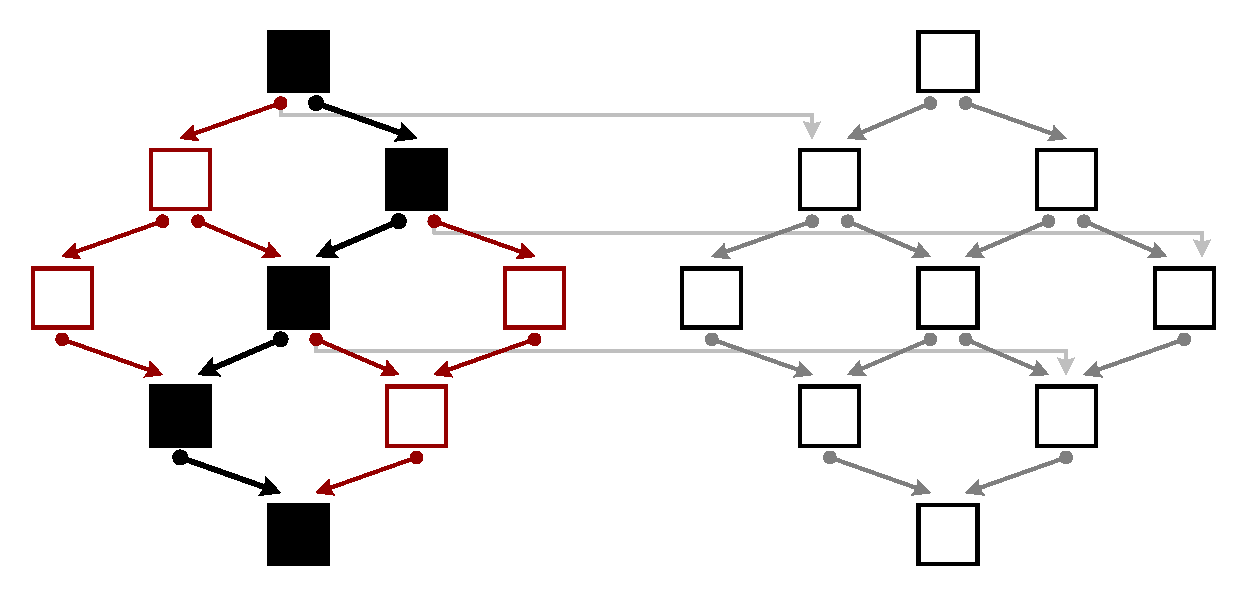
\includegraphics[width=0.9\textwidth]{./fig/vec_blackhole.pdf}
\singlespacing
\captionstyle{center}\caption{Иллюстрация схемы работы оптимизации <<черная дыра>>.}
\label{fig:text_4_vec_loc_branch_blackhole}
\end{figure}

Пусть дан некоторый CFG\label{abbr:cfg-2} тела плоского цикла (рис.~\ref{fig:text_4_vec_loc_branch_blackhole} слева), в котором присутствует явно выделенный пусть исполнения (на рисунке выделен черным цветом), вероятность прохождения которого близка к единице \cite{Shabanov2021VecCFG}.
Другие крайне маловероятные линейные участки (выделенные на рисунке красным цветом) представляют собой программный контекст, который практически никогда не исполняется, и векторизацию которого проводить нецелесообразно, либо невозможно.
Оптимизация blackhole заключается в создании точной копии CFG, на которую перенаправляются все маловероятные переходы из основного тела.
После выполнения перенаправления маловероятных переходов все ребра и линейные участки, отмеченные на рис.~\ref{fig:text_4_vec_loc_branch_blackhole} красным цветом, могут быть удалены.
Таким образом, после выполнения оптимизации в качестве объекта векторизации остается ограниченный и пригодный к векторизации программный контекст.
В случае же если один из маловероятных переходов все же осуществится, то выполнится переход на точную копию изначального CFG, который хоть и не оптимально, но корректно отработает эту редкую ситуацию.
Описанная оптимизация получила свое название blackhole, потому что после выполнения редкого перехода на копию CFG программа не может вернуться обратно в векторизованную версию, в этом случае исполняющийся экземпляр плоского цикла закончит свое исполнение в <<черной дыре>>.
Оптимизация может применяться в различных вариациях.
Например, можно создавать копию не целого CFG, а только конкретных маловероятных регионов, в этом случае мы будем иметь оптимизацию локализации редких путей исполнения.
Наоборот, более консервативным вариантом оптимизации является перенаправление маловероятных переходов сразу на голову невекторизованной копии тела цикла, что соответствует просто проведению повторного расчета при возникновении исключительной ситуации.

%---------------------------------------------------------------------------------------------------
% 5.5 - слияние

\subsection{Векторизация с помощью слияния путей исполнения}\label{sec:vec_mrg}

В этом разделе рассматривается оптимизация слияния путей исполнения по условию внутри плоского цикла с помощью постановки операций из параллельных скалярных блоков под предикаты этих блоков, трансформирующиеся при векторизации в векторные маски.
Приводятся аналитические оценки логической эффективности векторизации плоского цикла, в котором выполняется слияние двух скалярных блоков.

\subsubsection{Слияние по условию}\label{sec:text_4_vec_mrg_under_cond}

Универсальным способом векторизации программного кода, содержащего условия, является слияние всех путей исполнения под соответствующими предикатами \cite{Rybakov2024VecComb}.
Рассмотрим это действие на примере простого условия \texttt{cond}, по результату которого выполняется переход на один из блоков \texttt{block A} и \texttt{block B}.
Пусть известны вероятности переходов на эти блоки -- они равны $p$ и $1 - p$ соответственно.
Длины рассматриваемых блоков нормируем таким образом, чтобы в сумме они давали единицу, а отношение их длин задавалось параметром $\alpha$.
Таким образом, длины блоков будут равны $\frac{\alpha}{\alpha + 1}$ и $\frac{1}{\alpha + 1}$ соответственно (см. рис.~\ref{fig:text_4_vec_mrg_under_cond_cond}).
При этом условимся считать, что длина блока и время его исполнения это по сути одно и то же (то есть, время исполнения блока исчисляется количеством содержащихся в нем операций).

\begin{figure}[ht]
\centering
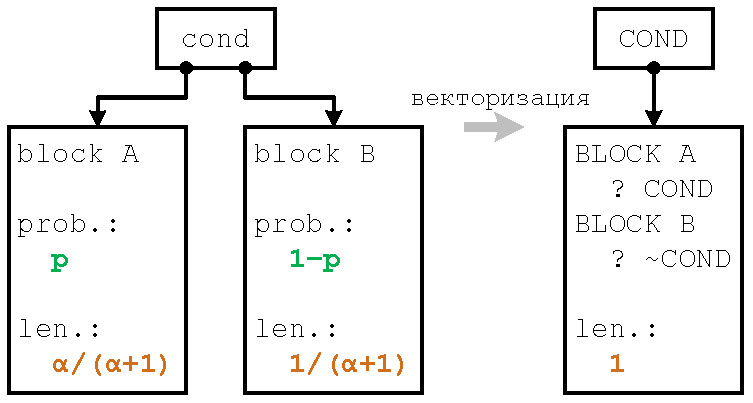
\includegraphics[width=0.7\textwidth]{./fig/vec_ifconv_nocheck.pdf}
\singlespacing
\captionstyle{center}\caption{Схема векторизации участка программного кода, состоящего из одного условия и двух блоков, переход на которые осуществляется в соответствии с этим условием.}
\label{fig:text_4_vec_mrg_under_cond_cond}
\end{figure}

Согласно представленной схеме программного контекста математическое ожидание времени исполнения рассматриваемых блоков в зависимости от условия, будет равно
\begin{equation}\label{eqn:text_4_vec_mrg_under_cond_t1}
	L = \frac{p \alpha}{\alpha + 1} + \frac{1 - p}{\alpha + 1} = p\left(\frac{\alpha - 1}{\alpha + 1}\right) + \left(\frac{1}{\alpha + 1}\right).
\end{equation}

Время выполнения $w$ таких участков кода в невекторизованном виде будет равно $wL$.
При векторизации кода необходимо избавиться от операций перехода, вместо этого все операции блоков \texttt{block A} и \texttt{block B} должны быть поставлены под предикаты \texttt{cond} и \texttt{\textasciitilde cond} соответственно.
Далее выполняется объединение $w$ участков кода, при котором скалярные операции под предикатами \texttt{cond}, \texttt{\textasciitilde cond} заменяются на векторные аналоги, выполняющиеся с использованием векторных масок \texttt{COND}, \texttt{\textasciitilde COND}.
Так как длины блоков выбирались таким образом, чтобы в сумме они давали единицу, то время исполнения векторной версии кода в точности равно $L_v = 1$.
Таким образом, логическая эффективность векторизации рассмотренного фрагмента кода совпадает со значением \eqref{eqn:text_4_vec_mrg_under_cond_t1} и равна
\begin{equation}\label{eqn:text_4_vec_mrg_under_cond_e}
	e_{vec}^{*} = \frac{L}{L_v} = p\left(\frac{\alpha - 1}{\alpha + 1}\right) + \left(\frac{1}{\alpha + 1}\right).
\end{equation}

На рис.~\ref{fig:text_4_vec_under_cond_chart_e_merged} представлены графики зависимостей логической эффективности векторизации из \eqref{eqn:text_4_vec_mrg_under_cond_e} для разных значений параметра $\alpha$.

\begin{figure}[ht]
\centering
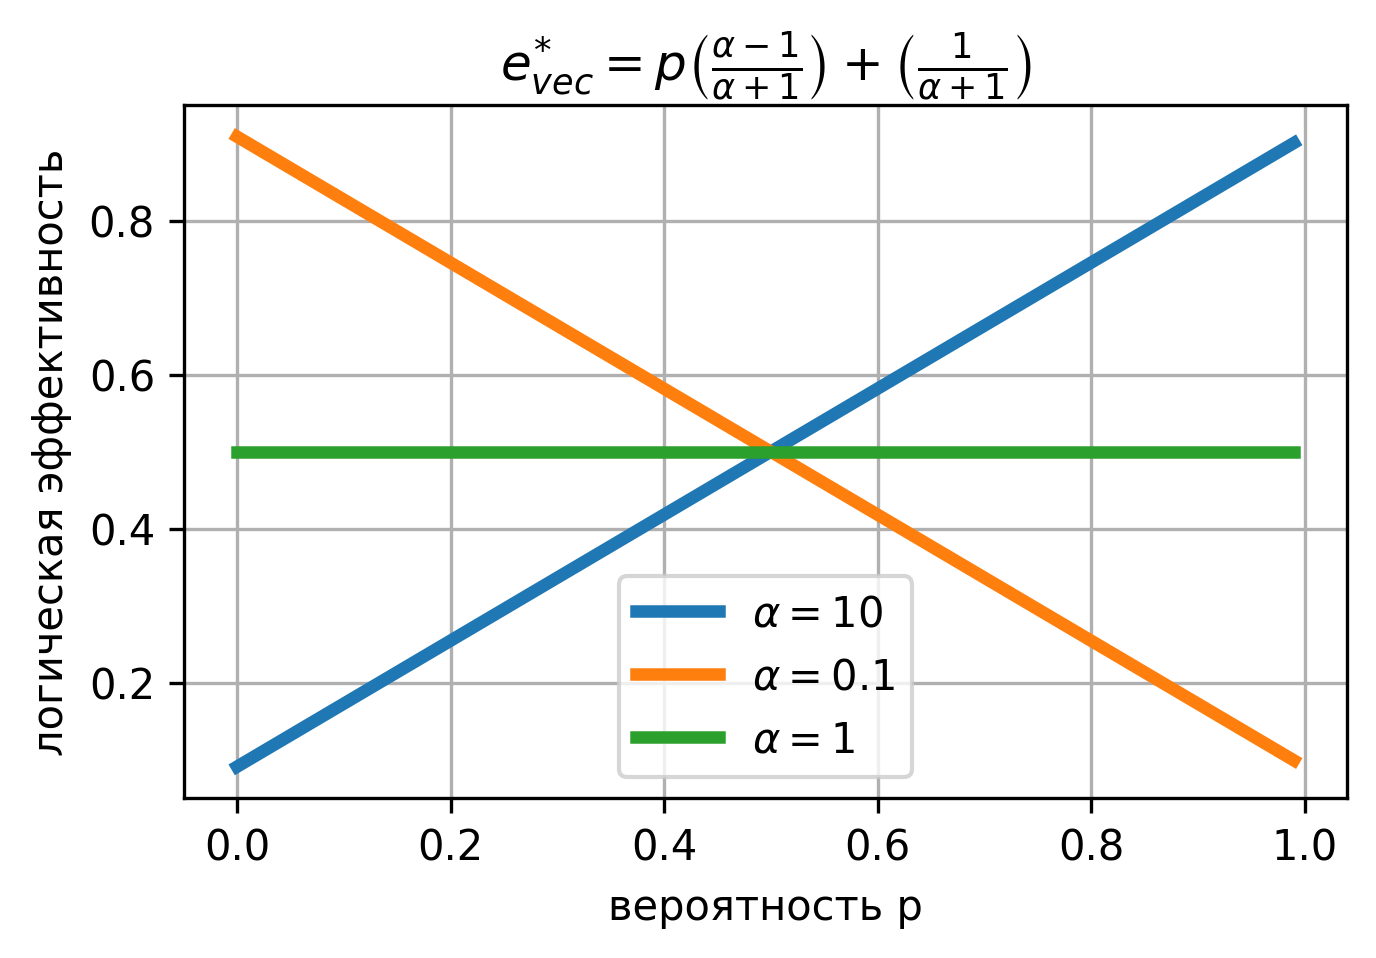
\includegraphics[width=0.6\textwidth]{./fig/vec_ifconv_nocheck_chart.png}
\singlespacing
\captionstyle{center}\caption{Графики зависимостей логической эффективности векторизации от вероятности перехода на \texttt{block A} при значениях отношения длин блоков \texttt{block A} и \texttt{block B} $\alpha = 10.0$, $\alpha = 0.1$, $\alpha = 1.0$ и при использовании простого слияния путей исполнения.}
\label{fig:text_4_vec_under_cond_chart_e_merged}
\end{figure}

Из рис.~\ref{fig:text_4_vec_under_cond_chart_e_merged} видно, что при $\alpha = 1$ (то есть при одинаковых длинах блоков \texttt{block A} и \texttt{block B}) эффективность векторизации постоянна и равна $0,5$.
В тех же случаях, когда длины блоков отличаются, эффективность векторизации возрастает, если вероятность перехода на более длинный блок выше, чем на более короткий блок.
В любом случае, можно констатировать, что такой подход прямого слияния ветвей исполнения под соответствующими предикатами в единый линейный участок является крайне неэффективным.
При возрастании количества условий эффективность векторизации таким способом падает экспоненциально.
Это связано с появлением в программном коде большого количества векторных инструкций с практически пустыми масками.
Для повышения эффективности векторизации контекста с условиями требуется рассмотрение других подходов, позволяющих повысить плотность масок исполняемых векторных команд.

% Проверка векторных масок исполняемого кода на пустоту.
\subsubsection{Слияние с проверкой масок на пустоту}\label{sec:text_4_vec_check_mask}

Рассмотрим модификацию слияния путей исполнения из раздела \ref{sec:text_4_vec_mrg_under_cond}, добавив проверку на пустоту векторых масок \texttt{COND} и \texttt{\textasciitilde COND}, под которыми исполняются векторизованные блоки \texttt{BLOCK A} и \texttt{BLOCK B} \cite{Rybakov2024VecComb} (см. рис.~\ref{fig:text_4_vec_check_mask_cond}). 

\begin{figure}[ht]
\centering
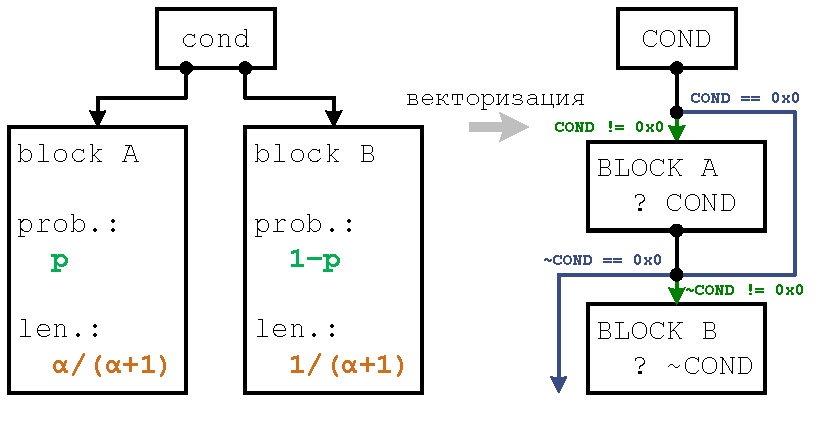
\includegraphics[width=0.7\textwidth]{./fig/vec_ifconv_check.pdf}
\singlespacing
\captionstyle{center}\caption{Схема векторизации участка программного кода, состоящего из одного условия и двух блоков, переход на которые осуществляется в соответствии с этим условием, с использованием проверок \\ векторных масок на пустоту.}
\label{fig:text_4_vec_check_mask_cond}
\end{figure}

Если векторная маска, под которой должен быть исполнен блок, пуста, то выполнять команды этого блока нет необходимости, поэтому проверка векторных масок на пустоту может повысить эффективность векторного кода.
Использование проверок векторных масок на пустоту оправдано, если вероятность появления пустых масок достаточно высока, а также исполняемый блок не является слишком коротким (в этом случае накладные расходы на лишнюю операцию сравнения и возможный переход нивелируют потенциальную пользу от применяемой оптимизации).
Скорректируем выражение для логической эффективности векторизации из \eqref{eqn:text_4_vec_mrg_under_cond_e} с учетом проверок векторных масок на пустоту.
Величина $L$ остается той же, что и в \eqref{eqn:text_4_vec_mrg_under_cond_t1}, а вот $L_v$ несколько изменится.
Если считать, что в каждом наборе обрабатываемых данных переход на тот или иной блок является случайной величиной, то вероятность пустой маски \texttt{COND} будет равна $(1 - p)^w$, тогда как вероятность пустой маски \texttt{\textasciitilde COND} равна $p^w$.
Тогда общая длина векторизованного кода может быть выражена как
\begin{equation}\label{eqn:text_4_vec_check_mask_tw}
	L_v = \left(1 - (1 - p)^w\right)\left(\frac{\alpha}{\alpha + 1}\right) + (1 - p^w)\left(\frac{1}{\alpha + 1}\right),
\end{equation}
а логическая эффективность векторизации примет следующий вид:
\begin{equation}\label{eqn:text_4_vec_check_mask_e}
	e_{vec}^{*} = \frac{ p(\alpha - 1) + 1 }{\left(1 - (1 - p)^w\right) \alpha + (1 - p^w) }.
\end{equation}

\begin{figure}[ht]
\centering
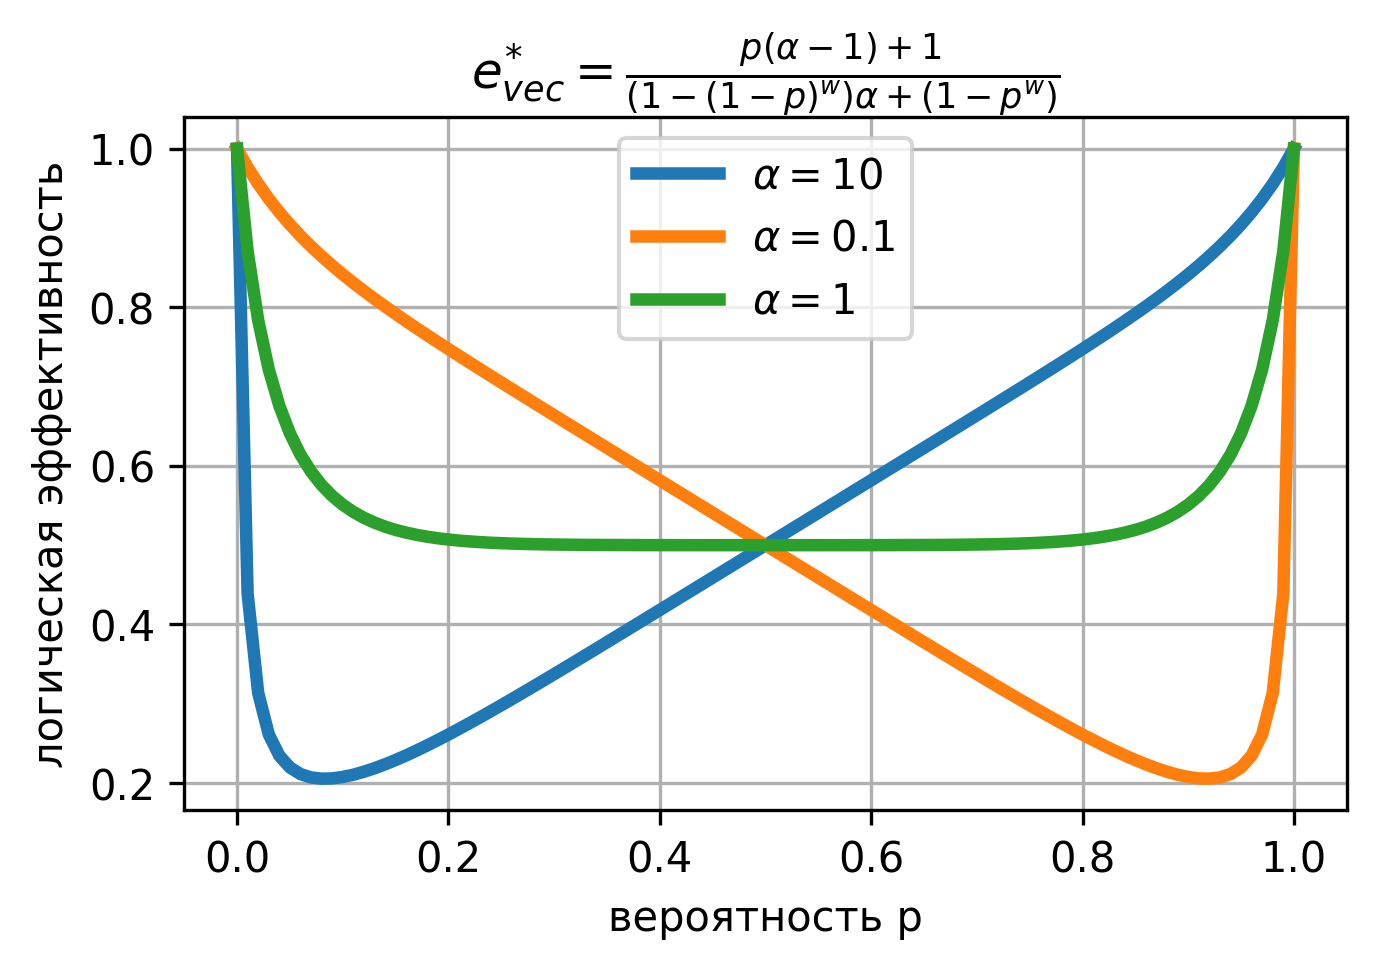
\includegraphics[width=0.6\textwidth]{./fig/vec_ifconv_check_chart.png}
\singlespacing
\captionstyle{center}\caption{Графики зависимостей логической эффективности векторизации от вероятности перехода на \texttt{block A} при значениях отношения длин блоков \texttt{block A} и \texttt{block B} $\alpha = 10.0$, $\alpha = 0.1$ и $\alpha = 1.0$ и при использовании слияния путей исполнения с проверкой масок на пустоту.}
\label{fig:text_4_vec_check_mask_chart_e_merged}
\end{figure}

На рис.~\ref{fig:text_4_vec_check_mask_chart_e_merged} представлены зависимости логической эффективности векторизации \eqref{eqn:text_4_vec_check_mask_e} при разных значениях параметра $\alpha$ с учетом проверок масок на пустоту для ширины векторизации $w = 16$, что соответствует использованию вещественного формата данных одинарной точности в 512-битных регистрах.

Из рис.~\ref{fig:text_4_vec_check_mask_chart_e_merged} видно, что эффективность векторизации возрастает, если значение вероятности перехода на один из блоков близко к единице, однако в среднем вероятность векторизации остается невысокой.

%---------------------------------------------------------------------------------------------------
% 5.6 - объединение и комбинирование

% Комбинирование векторных масок.
\subsection{Векторизация с объединением и комбинированием векторных масок}\label{sec:text_4_comb_mask}

При векторизации плоского цикла $w$ соседних скалярных итераций объединяются в один векторизованный векторный блок, таким образом $n$ итераций плоского цикла транформируются в $\lfloor \frac{n}{w} \rfloor$ векторных блоков без учета эпилога.
Слияние путей исполнения по условию порождает векторные блоки под векторными масками, таким образом образуются последовательности одинаковых векторных блоков под векторными масками.
В этом разделе рассматривается повышение плотности масок векторного кода с помощью объединения и комбинирования масок соседних векторных блоков.
В общем случае без учета комбинированных операций общее количество выполненных операций скалярного кода может быть выражено как $L = w \sum_{c \in C_v}{\rho(m(c))}$, где $C_v$ -- множество выполненных векторных инструкций в векторном коде, $m(c)$ -- маска инструкции, $\rho(m)$ -- плотность маски.
Таким образом, для повышения эффективности векторизации требуется повышение плостности векторных масок.

В общем случае можно считать, что в результате слияния под соответствующими предикатами ветвей исполнения внутри тела плоского цикла мы получим совокупность векторных блоков, обрабатывающихся сходим образом: загрузка входных данных \texttt{in\_data} под маской векторного блока, выполнение вычислений \texttt{block} под маской блока, сохранение результатов \texttt{out\_data} под маской блока (см. рис.~\ref{fig:text_4_vec_comb_mask_vec_block}).
На этой схеме \texttt{in\_data} и \texttt{out\_data} могут являться как одиночными векторами, так и наборами векторов.

\begin{figure}[ht]
\centering
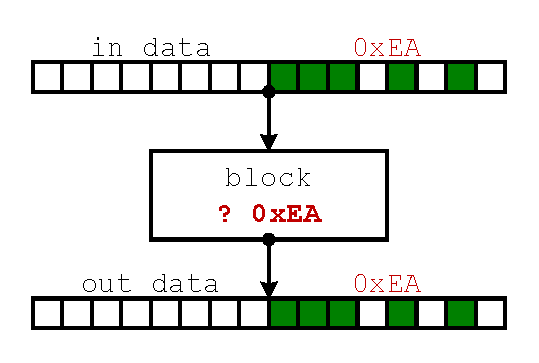
\includegraphics[width=0.5\textwidth]{./fig/vec_block_under_mask.pdf}
\singlespacing
\captionstyle{center}\caption{Схема вычислений векторизованного блока команд с входными данными \texttt{in\_data}, выходными данные \texttt{out\_data} и маской исполнения \texttt{0xEA}.}
\label{fig:text_4_vec_comb_mask_vec_block}
\end{figure}

Проверка маски блока на пустоту может повысить эффективность кода, если маски часто оказываются пустыми.
Однако этот никак не поможет в том случае, если в маске выставлено несколько битов.
В некоторых случаях достичь повышения производительности можно путем объединения двух соседних векторных блоков \cite{Rybakov2024VecComb}.

\subsubsection{Объединение непересекающихся масок}

Если в процессе векторизации у нас появились два соседних векторных блока \texttt{block(in\_data\_1)} $\rightarrow$ \texttt{out\_data\_1} и \texttt{block(in\_data\_2)} $\rightarrow$ \texttt{out\_data\_2}, которые должны выполняться под разными векторными масками \texttt{mask\_1} и \texttt{mask\_2}, и в дополнение к этому для этих масок выполнено условие \texttt{(mask\_1 \& mask\_2) == 0x0} (то есть маски не пересекаются), то вычисление этих двух соседних блоков можно объединить.
Вместо последовательного выполнения двух векторных блоков можно объединить их входные данные \texttt{in\_data\_1} и \texttt{in\_data\_2} с помощью слияния \texttt{in\_data = \_mm512\_mask\_blend\_ps(mask\_1, in\_data\_2, in\_data\_1}), после чего выполнить тот же блок вычислений под маской \texttt{mask\_1 | mask\_2}.
Ввиду отсутствия пересечения векторных масок в результирующих выходных данных \texttt{out\_data} будут содержаться как необходимые элементы данных \texttt{out\_data\_1}, так и необходимые элементы данных \texttt{out\_data\_2}.
В конце остается извлеч из объединенного результата \texttt{out\_data} данные \texttt{out\_data\_1} и \texttt{out\_data\_2} (см. рис.~\ref{fig:text_4_vec_comb_mask_comb_masks}).

\begin{figure}[ht]
\centering
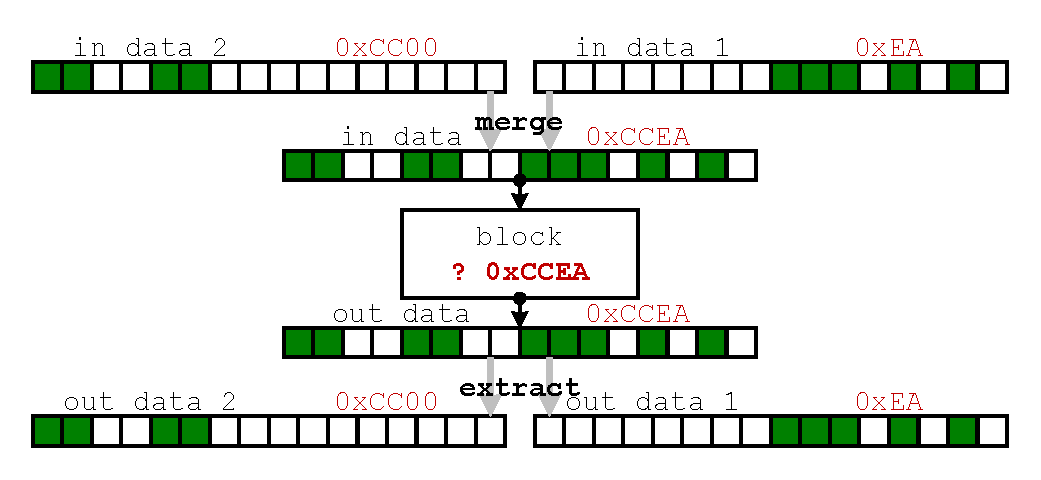
\includegraphics[width=1.0\textwidth]{./fig/vec_masks_union.pdf}
\singlespacing
\captionstyle{center}\caption{Схема вычислений с объединением двух векторизованных блоков \texttt{block(in\_data\_1)} $\rightarrow$ \texttt{out\_data\_1}, \texttt{block(in\_data\_2)} $\rightarrow$ \texttt{out\_data\_2}.
Объединение допустимо, так как векторные маски \texttt{0xCC00} и \texttt{0xEA} не пересекаются, объединенный блок выполняется под маской \texttt{0xCCEA}.}
\label{fig:text_4_vec_comb_mask_comb_masks}
\end{figure}

В результате такого преобразования в случае отсутствия пересечения векторных масок количество вычислений рассматриваемого блока \texttt{block} сокращается вдвое, а плотность векторных масок внутри блока повышается.
Однако вместе с этим появляются накладные расходы, связанные с проверками масок, а также операции слияния данных до вычислений блока и выделения нужных данных после вычислений.
Заметим, что эту технику можно применять для объединения трех и более соседних блоков, однако это связано с еще большим возрастанием накладных расходов.

\subsubsection{Комбинирование пересекающихся масок}

Еще один подход, о котором стоит упомянуть, но который не проверялся с точки зрения эффективности, связан с объединением соседних блоков с пересекающимися масками, то есть для которых \texttt{(mask\_1 \& mask\_2) != 0x0}.

\begin{figure}[ht]
\centering
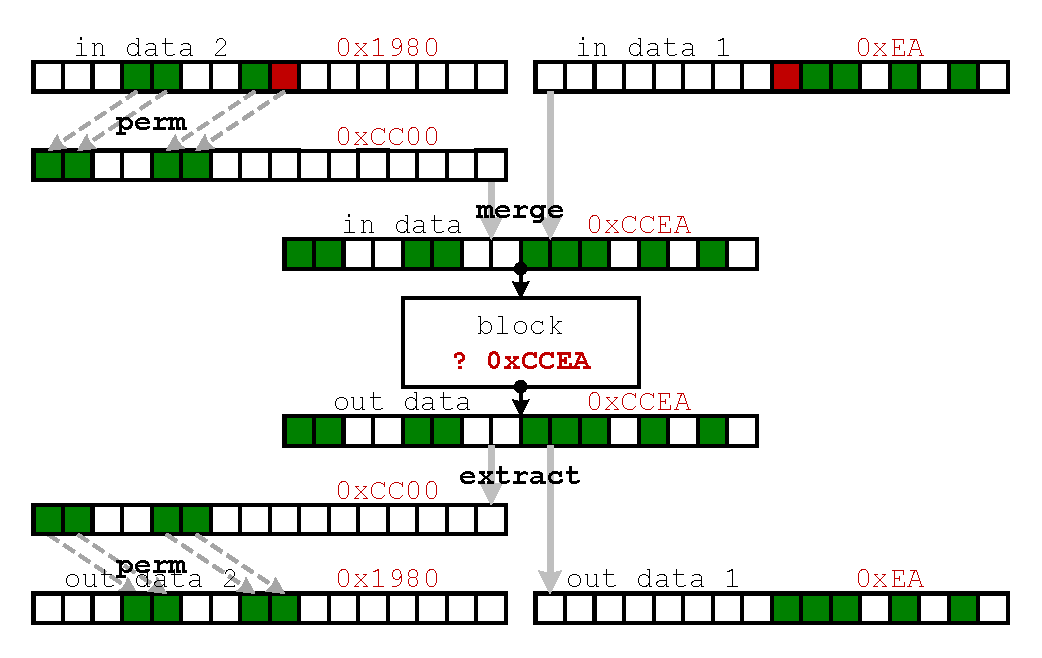
\includegraphics[width=1.0\textwidth]{./fig/vec_masks_comb.pdf}
\singlespacing
\captionstyle{center}\caption{Схема вычислений с объединением двух векторизованных блоков при условии пересечения их масок. Для объединения применяется изменение порядка элементов в данных одного из блоков.}
\label{fig:text_4_vec_comb_mask_comb_masks_perm}
\end{figure}

Если мы имеем дело с двумя масками низкой плотности, которые пересекаются, но для которых выполнено условие непревышения суммарной плотности ширины векторизации \texttt{popcnt(mask\_1) + popcnt(mask\_2) <= w}, то такие блоки также можно объединить.
Для этого перед объединением необходимо применять преобразование одной или обеих масок.

\begin{definition}
Преобразование \texttt{perm\_to} векторной маски \texttt{mask} называется обратимым, если существует преобразование \texttt{perf\_from} такое, что \texttt{perm\_from(perm\_to(mask)) = mask}.
\end{definition}

Для выполнения комбинирования векторных масок двух соседних блоков необходимо найти обратимое преобразование одной из масок (например, \texttt{mask\_1}) \texttt{perm\_to} такое, что будет выполнено условие \texttt{(perm\_to(mask\_1) \& mask\_2) == 0x0}.
В этом случае элементы входных данных переставляются местами в соответствии с преобразованием \texttt{perm\_to}, применяется описанная выше техника объединения блоков, а для выходных данных выполняется перестановка элементов в соответствии с преобразованием \texttt{perm\_from} (см. рис.~\ref{fig:text_4_vec_comb_mask_comb_masks_perm}).

Отметитм следующие моменты.
Объединять можно не только два соседние блока, но также три и более, но это усложняет программный код и увеличивает накладные расходы.
Следует принимать во внимание доступные операции по изменению порядка расположения элементов векторов, так как таких операций достаточно много и они отличаются по времени выполнения (SHUF, UNPCK, VPERM, VPERMIL и другие).
Преобразование исходных масок можно применять не к одной из них, а сразу к обеим маскам.
В этом случае необходимо найти обратимое преобразование первой маски \texttt{perm\_to\_1} и обратимое преобразование второй маски \texttt{perm\_to\_2}, такие что будет выполнено условие \texttt{(perm\_to\_1(mask\_1) \& perm\_to\_2(mask\_2)) = 0x0}.

\subsubsection{Эксперимент по объединению векторных масок}\label{sec:text_4_comb_mask_analyze}

В качестве примера, на котором проводился анализ эффективности векторизации плоских циклов с использованием объединения непересекающихся масок соседних векторизованных блоков, рассмотрим одну из функций реализации газодинамического римановского решателя -- функцию \texttt{prefun}.

\begin{singlespace}
\begin{lstlisting}[caption={Скалярная версия функции \texttt{prefun} из состава \\ римановского решателя.},label={lst:text_4_vec_comb_prefun_scalar}]
void scase_prefun_1(float& f, float& fd,
                    float p, float dk, float pk, float ck)
{
    if (p <= pk)
    {
        float prat = p / pk;
        f = riemann::sg4 * ck * (pow(prat, riemann::sg1) - 1.0f);
        fd = (1.0f / (dk * ck)) * pow(prat, -riemann::sg2);
    }
    else
    {
        float ak = riemann::sg5 / dk;
        float bk = riemann::sg6 * pk;
        float qrt = sqrt(ak / (bk + p));
        f = (p - pk) * qrt;
        fd = (1.0f - 0.5f * (p - pk) / (bk + p)) * qrt;
    }
}
\end{lstlisting}
\end{singlespace}

Для удобства будем пользоваться реализацией этой функции на языке программирования C \cite{riemannvecGithub}, как это представлено на листинге~\ref{lst:text_4_vec_comb_prefun_scalar}.

Функция \texttt{prefun} на листинге~\ref{lst:text_4_vec_comb_prefun_scalar} обрабатывает набор скалярных данных \texttt{p}, \texttt{dk}, \texttt{pk}, \texttt{ck} и вычисляет выходные аргументы \texttt{f}, \texttt{fd}.
Функция содержит одно условие и две ветви исполнения.
Обе ветви исполнения содержат достаточно тяжелые вычисления, что делает оправданным применение проверки масов на пустоту.
Все задействованные в реализации функции операции имеют векторные аналоги в наборе инструкций AVX-512\label{abbr:avx-11} (точнее в наборе функций-интринсиков), поэтому приведенная функция может быть векторизована путем замены скалярных операций векторными аналогами и слияния ветвей исполнения под соответствующими предикатами, как это показано на листинге~\ref{lst:text_4_vec_comb_prefun_vec}.

\begin{singlespace}
\begin{lstlisting}[caption={Векторизованная версия функции \texttt{prefun} из состава римановского решателя.},label={lst:text_4_vec_comb_prefun_vec}]
void vcase_prefun_1(__m512& f, __m512& fd,
                    __m512& p, __m512& dk, __m512& pk, __m512& ck,
                    __mmask16 m)
{
  __mmask16 cond = _mm512_kand(_mm512_cmple_ps_mask(p, pk), m);
  __mmask16 ncond = _mm512_kand(_mm512_knot(cond), m);

  { // first branch
    __m512 prat = _mm512_mask_div_ps(zero, cond, p, pk);
    f = _mm512_mask_mul_ps(f, cond,
          _mm512_mask_mul_ps(zero, cond, riemann::g4, ck),
          _mm512_mask_sub_ps(zero, cond,
            _mm512_mask_pow_ps(zero, cond, prat, riemann::g1),
            one));
    fd = _mm512_mask_mul_ps(fd, cond,
           _mm512_mask_div_ps(zero, cond, one,
             _mm512_mask_mul_ps(zero, cond, dk, ck)),
           _mm512_mask_pow_ps(zero, cond, prat,
             _mm512_mask_sub_ps(zero, cond, zero, riemann::g2)));
  }
  { // second branch
    __m512 ak = _mm512_mask_div_ps(zero, ncond, riemann::g5, dk);
    __m512 bk = _mm512_mask_mul_ps(zero, ncond, riemann::g6, pk);
    __m512 qrt = _mm512_mask_sqrt_ps(zero, ncond,
                   _mm512_mask_div_ps(zero, ncond, ak,
                     _mm512_mask_add_ps(zero, ncond, bk, p)));
      f = _mm512_mask_mul_ps(f, ncond,
            _mm512_mask_sub_ps(zero, ncond, p, pk), qrt);
      fd = _mm512_mask_mul_ps(fd, ncond,
             _mm512_mask_sub_ps(zero, ncond, one,
               _mm512_mask_mul_ps(zero, ncond, half,
                 _mm512_mask_div_ps(zero, ncond,
                   _mm512_mask_sub_ps(zero, ncond, p, pk),
                   _mm512_mask_add_ps(zero, ncond, bk, p)))),
             qrt); 
  }
}                 
\end{lstlisting}
\end{singlespace}

В процессе векторизации не применялись никакие локальные оптимизации, все скалярные операции были строго заменены на векторные аналоги с сохранением порядка вычислений с точности до ассоциативности умножения.
Из приведенного на листинге~\ref{lst:text_4_vec_comb_prefun_vec} кода видно, что команды первой ветви выполняются под маской \texttt{cond}, а другой ветви -- под маской \texttt{ncond}, таким образом можно применить проверку масок на пустоту.

Когда в разделе~\ref{sec:vec_mrg} вычислялась вероятность появления пустой маски, то использовалось предположение, что выполнение условий для разных наборов скалярных данных являются независимыми событиями.
На самом деле это не так и существенным образом зависит от локальности размещения данных, участвующих в расчетах \cite{Rybakov2020VecMon}.
Рассмотрим более подробно условие \texttt{p <= pk}.
Элементы данных \texttt{p} и \texttt{pk} свои для каждой расчетной ячейки.
Если речь идет о физических расчетах (а функция prefun относится к газодинамическому решателю), то значение элемента данных изменяется не слишком сильно при переходе от одной ячейки к соседней ячейке (см. рис.~\ref{fig:text_4_vec_comb_continuity}).

\begin{figure}[ht]
\centering
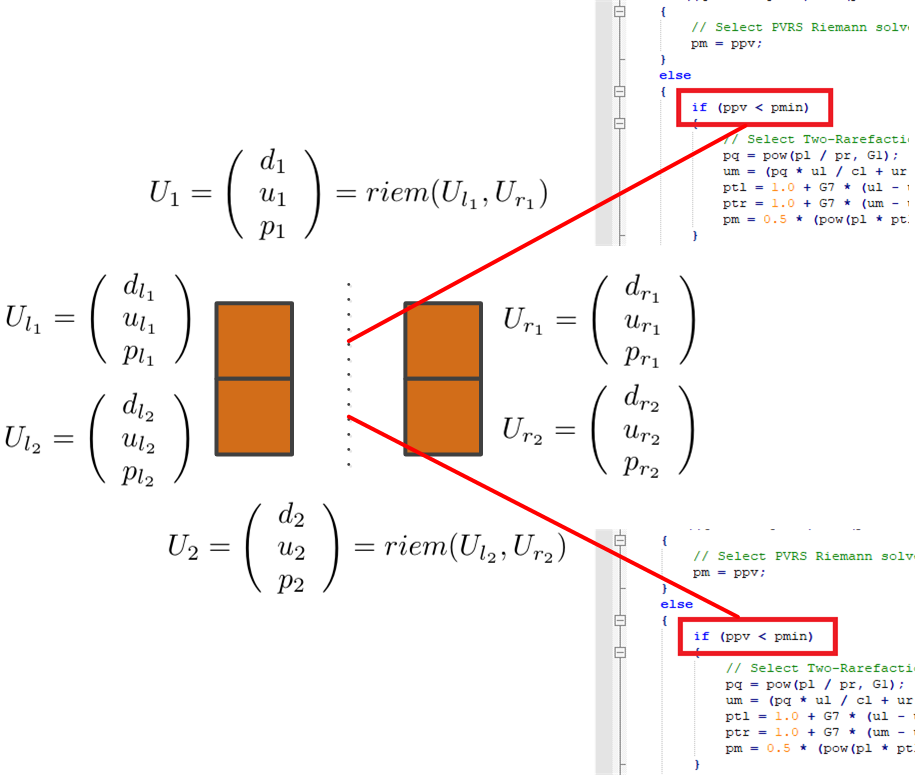
\includegraphics[width=0.6\textwidth]{fig/vec_continuity.png}
\singlespacing
\captionstyle{center}\caption{Иллюстрация тенденции сохранения значения условия при переходе к соседним ячейками в расчетных задачах.}
\label{fig:text_4_vec_comb_continuity}
\end{figure}

Значение условия \texttt{p <= pk} при переходе от одной ячейки к соседней будет изменяться также не слишком быстро.
Но условие это дискретная величина, а это значит, что часто значение условия будет сохраняться при переходе к соседней ячейке.
Для рассматриваемой функции \texttt{prefun} были собраны расчетные данные распределения плотности маски условия \texttt{p <= pk}, чтобы оценить вероятность появления пустых масок \texttt{cond} и \texttt{ncond}.
На рис.~\ref{fig:text_4_vec_comb_mask_independent_p} слева представлено распределение плотности масок в случае независимости условий для разных наборов скалярных данных.
Результаты распределения плотности маски \texttt{cond}, собранные по настоящему профилю исполнения векторного кода на реальных данных, представлены на рис.~\ref{fig:text_4_vec_comb_mask_independent_p} справа.

\begin{figure}[ht]
\centering
\begin{tabular}{ll}
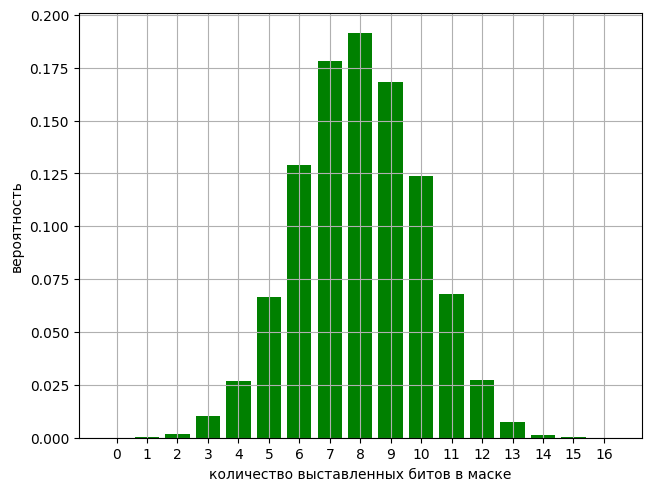
\includegraphics[width=0.45\textwidth]{fig/vec_mask_distr_independent_p.png}
&
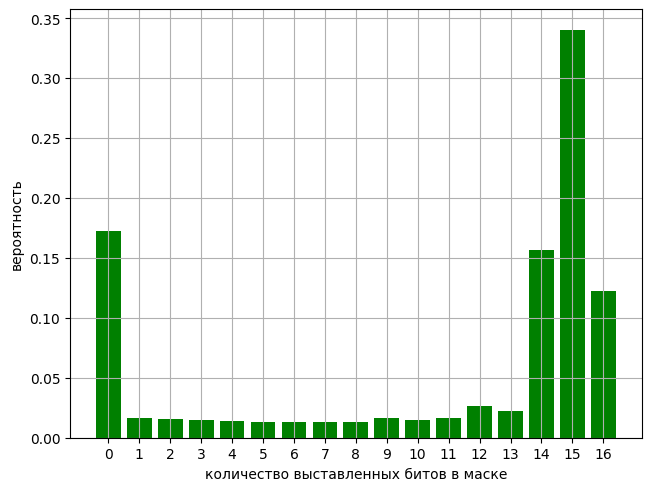
\includegraphics[width=0.45\textwidth]{fig/vec_mask_distr_real_p.png}
\end{tabular}
\singlespacing
\captionstyle{center}\caption{Гистограмма распределения количества единичных битов маски \texttt{cond} при условии, что все условия \texttt{p <= pk} для наборов скалярных данных являются независимыми (слева) и на реальном профиле исполнения (справа).}
\label{fig:text_4_vec_comb_mask_independent_p}
\end{figure}

Из рис.~\ref{fig:text_4_vec_comb_mask_independent_p} видно, что распределение плотностей масок на реальных данных совершенно не похоже на распределение, вычисленное в предположении о независимости условий переходов.
Можно заметить, что в реальном коде более четверти всех масок \texttt{cond} являются либо пустыми, либо полными (в этом случае пустой является маска \texttt{ncond}), а значит использование проверок масок на пустоту обосновано.

Для анализа полученных результатов были рассмотрены следующие три подхода к векторизации плоского цикла с условием.
В качестве базового метода векторизация принималось простое слияние путей исполнения под соответствующими предикатами с последующим объединением $w$ последовательных скалярных итераций в одну векторную (простое слияние).
Этот базовый метод сравнивался с двумя рассмотренными выше улучшениями: проверка масок блоков на пустоту (проверка масок) и слияние двух соседних блоков при условии отсутствия пересечения их масок (объединение масок).
Анализ эффективности применения преобразований рассматривался на приведенной в листинге~\ref{lst:text_4_vec_comb_prefun_scalar} функции \texttt{prefun} из реализации газодинамического римановского решателя.
Профиль исполнения функции собирался на задачах моделирования распада разрыва при различных начальных условиях \cite{Toh2024VecRiemann,Zeng2021VecRiemann}.
Эффективность векторизации при выбранных подходах измерялась двумя способами.
В качестве первого способа использовался режим эмуляции векторных инструкций.
В настоящее время используются различные эмуляторы AVX-512 с помощью которых можно оценить эффективность векторного кода \cite{Lee2024VecGem}.
При анализе рассматриваемой функции мы ограничились инструментом, позволяющим отследить плотность используемых в коде масок и общее количество скалярных и векторных операций \cite{Rybakov2023VecShvindt}.
Вторым способом сравнения был замер производительности результирующего векторного кода на микропроцессоре Intel Xeon Phi KNL.
Результаты сравнения представлены на рис.~\ref{fig:text_4_vec_comb_mask_res}.

\begin{figure}[ht]
\centering
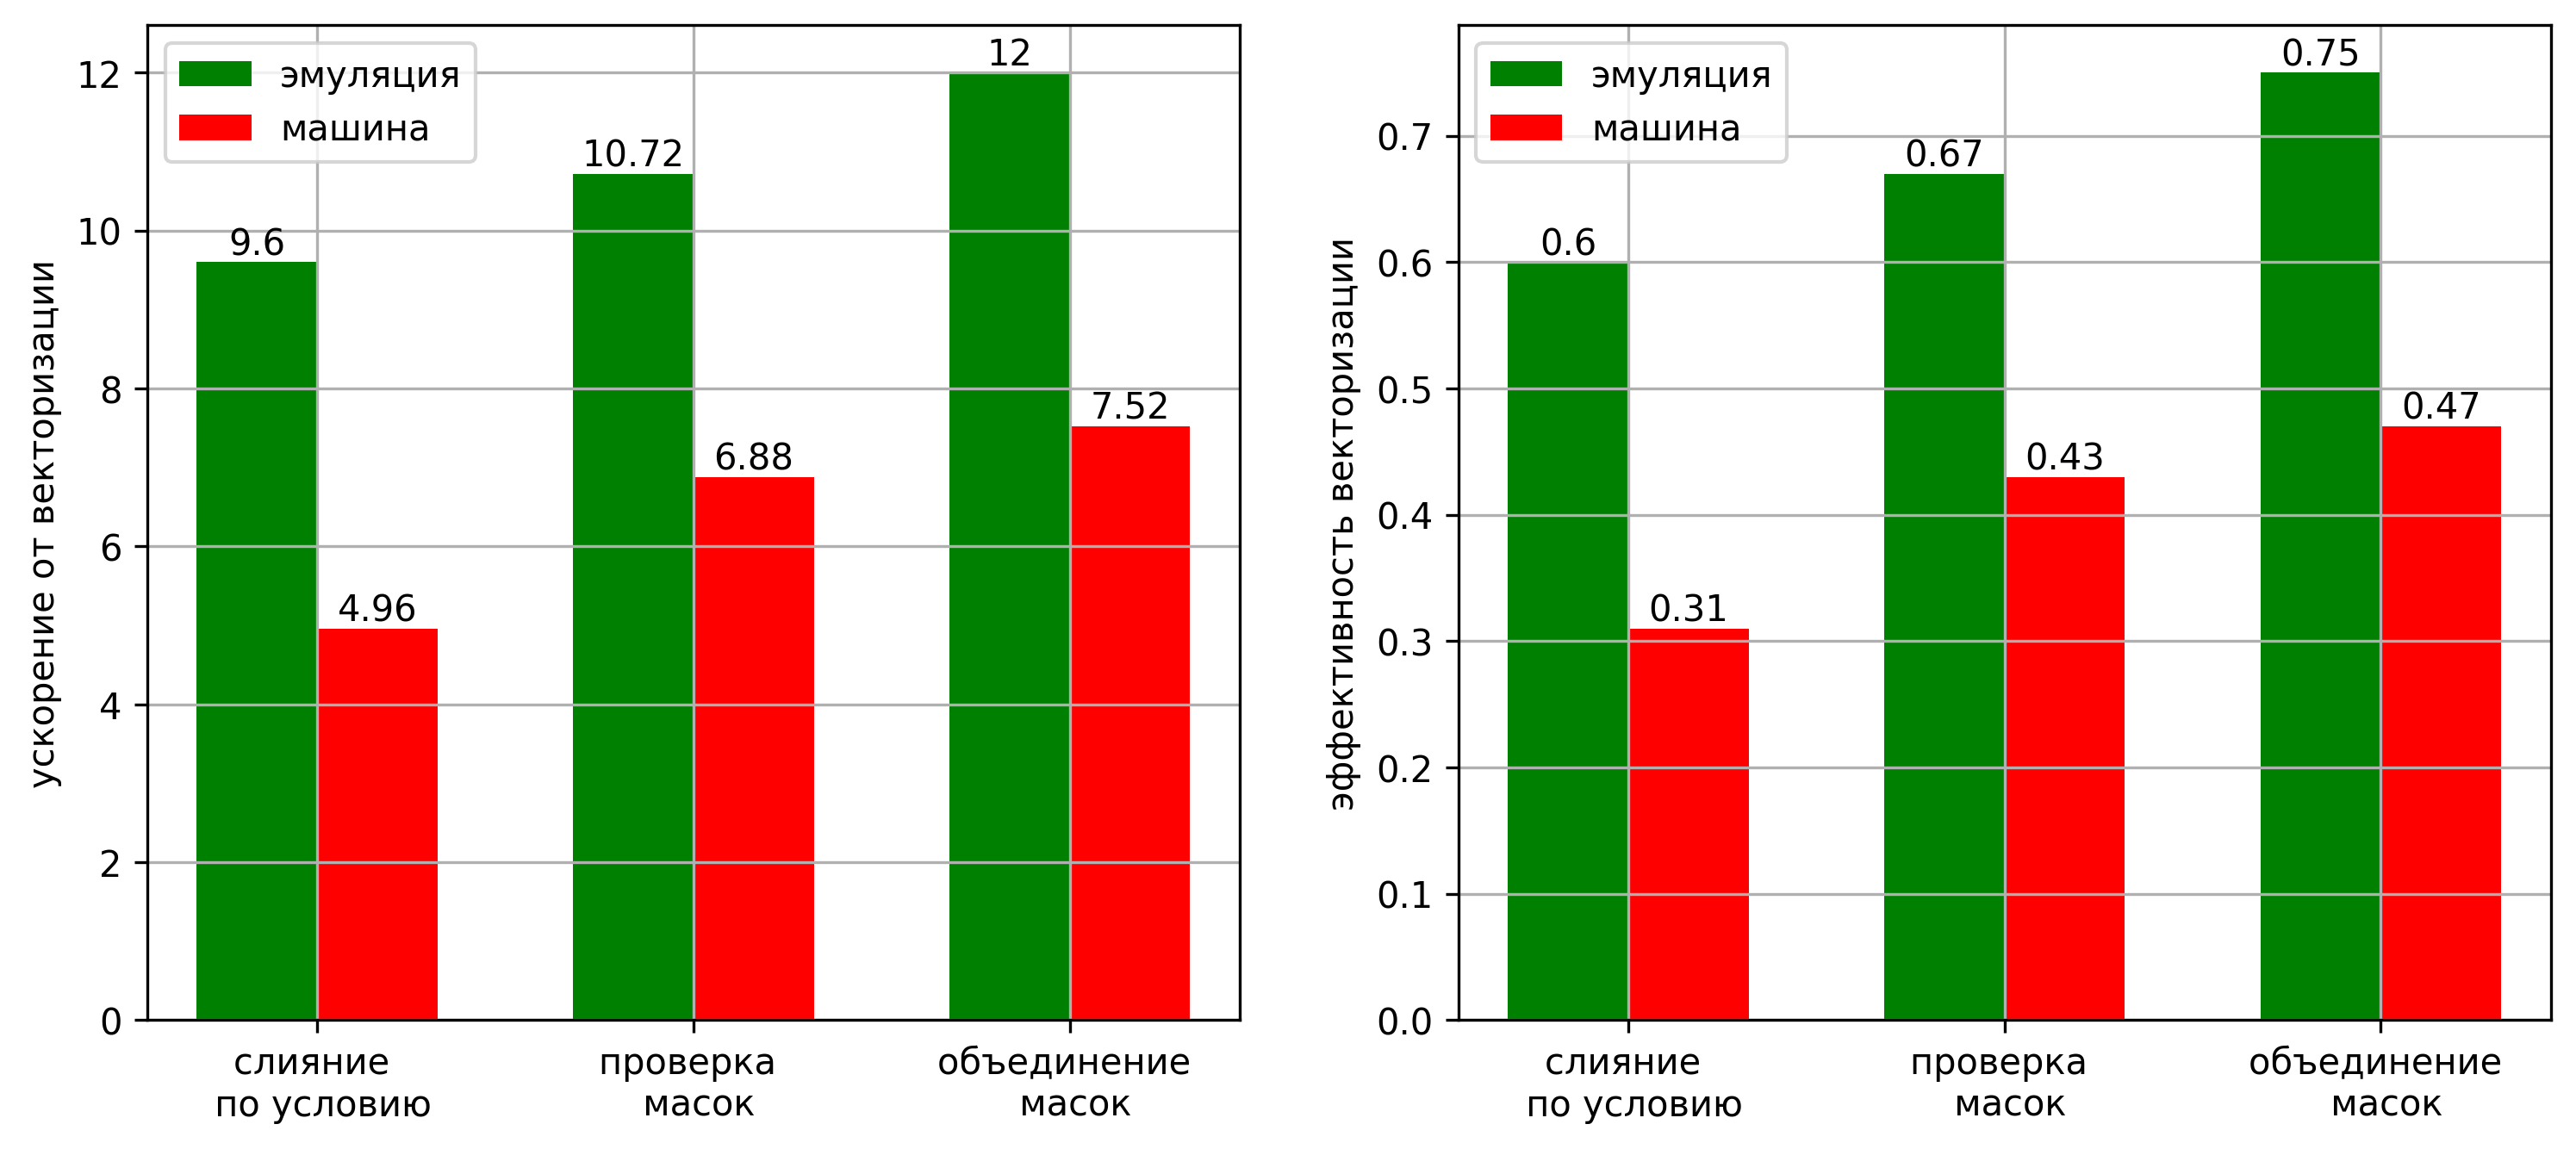
\includegraphics[width=1.0\textwidth]{./fig/vec_masks_union_res.png}
\singlespacing
\captionstyle{center}\caption{Результаты сравнения эффективности векторизации при простом слиянии, с проверкой масок и с объединением масок в режимах эмуляции и на микропроцессоре Intel Xeon Phi KNL\label{abbr:knl-9}.}
\label{fig:text_4_vec_comb_mask_res}
\end{figure}

Эксперимент показал, что в режиме эмуляции слияние ветвей исполнения привело к эффективности векторизации 0,6.
Использование проверки масок и объединения масок позволило пвысить ее до 0,67 и 0,75 соответственно.
На реальной машине простое слияние путей исполнения позволило достичь эффективности 0,31, а использование проверок масок и объединения масок позволило повысить ее до 0,43 и 0,47 соответственно.

%---------------------------------------------------------------------------------------------------
% 5.7 - гнезда циклов

\subsection{Векторизация гнезд циклов}

В расчетных приложениях часто встречается код, в котором тело плоского цикла содержит другие циклы или гнезда циклов.
В этом разделе проводится анализ программного контекста, в котором тело плоского цикла содержит другой цикл, такую конструкцию будем называть <<плоский цикл / внутренний цикл>> (см. рис.~\ref{fig:vec_flat_loop_nest}).

\begin{figure}[!ht]
\centering
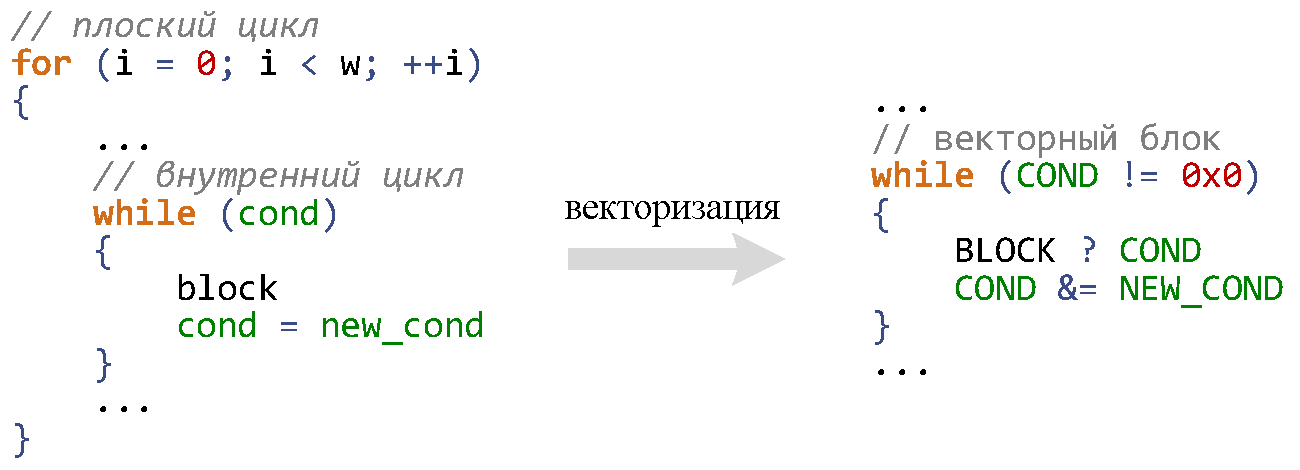
\includegraphics[width=0.85\textwidth]{fig/vec_flat_loop_nest.pdf}
\singlespacing
\caption{Схема векторизации стуктуры <<плоский цикл / внутренний цикл>>.}
\label{fig:vec_flat_loop_nest}
\end{figure}

При выполнении векторизации тело внутреннего цикла $block$, выполняемое по условию $cond$, переводится в векторный блок $BLOCK$, инструкции которого выполняются под маской $COND$, которая постепенно истощается пока не станет равной \texttt{0x0}.
При этом выполняется соотношение $I_v = \max_{i = 0}^{w - 1}{I(i)}$, где $I(i)$ -- количество итераций внутреннего цикла на $i$-ой итерации плоского цикла в скалярной версии, $I_v$ -- количество итераций внутреннего цикла в векторизованной версии.
Эффективность векторизации рассматриваемого программного кода зависит от характера изменения условия $cond$ (и соответственно количества итераций внутреннего цикла $I(i)$) при переходе между итерациями плоского цикла.
Слишком резкое изменения условия $cond$ между итерациями плоского цикла приводит к сильному изменению значений $I(i)$, что приводит к деградации производительности при векторизации структруры <<плоский цикл / внутренний цикл>>.
В терминах количества итераций справедлива следующая лемма.

\begin{lemma}\label{lem:vec_lem}
При векторизации структуры <<плоский цикл / внутренний цикл>>, верна априорная оценка
\begin{equation}\label{eqn:vec_7_lemma_eqn_1}
e_{vec}^{*} \le e_{vec}^I,
\end{equation}
где $e_{vec}^I = \frac{ \sum_{i = 0}^{w - 1}{I(i)} }{I_v w}$.
При этом, если $I_v - \min_{i = 0}^{w - 1}{I(i)} \le \epsilon$, то
\begin{equation}\label{eqn:vec_7_lemma_eqn_2}
e_{vec}^I \ge 1 - \frac{\epsilon}{I_v}.
\end{equation}
\end{lemma}

Пусть $\lambda$ -- количество операций на одной итерации внутреннего цикла в скалярной версии, а $\lambda_v$ -- количество операций на одной итерации внутреннего цикла в векторной версии, при этом $\frac{\lambda}{\lambda_v} \le 1$ (равенство достигается при идеальной векторизации итерации внутреннего цикла.
Из этого следует оценка \eqref{eqn:vec_7_lemma_eqn_1}, так как
\begin{equation}
	e_{vec}^{*} = \frac{L}{L_v w} = \frac{\sum_{i = 0}^{w - 1}{\sum_{j = 0}^{I(i) - 1}{\lambda}}}{w \sum_{j = 0}^{I_v}{\lambda_v}} = \frac{\lambda \sum_{i = 0}^{w - 1}{I(i)}}{w \lambda_v I_v} = \frac{\lambda}{\lambda_v} e_{vec}^I \le e_{vec}^I.
\end{equation}

Так как $I_v - \min_{i = 0}^{w - 1}{I(i)} \le \epsilon$, то $\forall i \in [0, w - 1] \implies I(i) \ge I_v - \epsilon$, откуда следует вторая оценка
\begin{equation}
	e_{vec}^I = \frac{\sum_{i = 0}^{w - 1}{I(i)}}{I_v w} \ge \frac{(I_v - \epsilon) w}{I_v w} = 1 - \frac{\epsilon}{I_v}. \ \blacksquare
\end{equation}

Параметр $\epsilon$ из леммы~\ref{lem:vec_lem} можно назвать коэффициентом неравномерности распределения количества итераций внутреннего цикла в скалярной версии (если $\epsilon = 0$, то все $I(i)$ равны между собой).
Далее в разделе рассмотрены различные варианты характера изменения условий $cond$ в стурктуре <<плоский цикл / внутренний цикл>> и распределения количества итераций внутреннего цикла в скалярной версии, и влияние этих факторов на эффективность векторизации.

\subsubsection{Внутренний циклов с постоянным количеством итераций}\label{sec:text_4_vec_mesh_intersect}

В этом разделе рассматривается наиболее простой случай, когда внутренний цикл, находящийся в теле плоского цикла, выполнятеся с постоянным количеством итераций, то есть $\epsilon = 0$ и $e_{vec}^I = 1$.

В разделе~\ref{sec:text_1_immersed_boundary_method} был описан метод погруженных границ для выполнения газодинамических расчетов вокруг тела со сложной геометрией.
Первым этапом его реалиазации, описанным в разделе~\ref{sec:text_1_immersed_boundary_method_realization}, является поиск пересечения всех ячеек неструктурированной поверхностной расчетной сетки со всеми ячейками объемной декартовой сетки.
Для решения этой задачи требуется многократно выполнить процедуру обнаружения пересечения треугольника и прямоугольного параллелепипеда в пространстве, эта процедура описана в разделе~\ref{sec:int_with_undermesh}.
Если задать координаты точек, образующих ячейки рассматриваемых расчетных сеток в виде набора массивов координат, то задачу поиска пересечений между парами ячеек (треугольник -- прямоугольный параллелепипед) можно организовать в виде плоского цикла, телом которого будет являться установление факта пересечения одной пары ячеек.
Рассмотрим подход к векторизации этого программного контекста \cite{Rybakov2019VecInt}.

Рассмотрим реализацию функции \texttt{tri\_box\_intersect}, анализирующую наличие пересечения треугольника и прямоугольного параллелепипеда с помощью метода свертывания системы линейных неравенств из \cite{Chernikov1963} (см. листинг~\ref{lst:text_1_mesh_intersect_tri}).

Функция возвращает $1$, если пересечение есть, и $0$, если пересечения нет.
Логика работы функции следующая.
Сначала коэффициенты системы неравенств \eqref{eqn:text_1_geo_prim_2} заносятся в двумерный массив коэффициентов \texttt{g[bec][3]}, где \texttt{bec} (basic equations count) -- количество исходных неравенств системы (в нашем случае 9).
Затем выполняется один шаг деформации системы с одновременным поиском множества решения для переменной $\gamma$.
Перед началом свертывания множество допустимых значений для переменной $\gamma$ принимается в виде отрезка $[0, 1]$ (\texttt{lo = 0}, \texttt{hi = 1}).
По мере свертывания системы неравенств \eqref{eqn:text_1_geo_prim_2} происходит сокращение множеств решений.
Если на каком-то этапе свертывания множество решений обращается в пустое (\texttt{lo > hi}), то функция заканчивает работу и возвращает 0.
Если после выполнения всех действий свертывания множество решений осталось ненулевым, то это означает наличие пересечения, и функция возвращает 1.

\begin{singlespace}
\begin{lstlisting}[caption={Исходная реализация свертывания системы линейных неравенств для определения пересечения треугольника и прямоугольного параллелепипеда.},label={lst:text_1_mesh_intersect_tri}]
for (i = 0; i < bec; ++i)
{
    gi0 = g[i][0];

    if (gi0 == 0.0)
    {
        if (!upgrade(g[i][1], g[i][2], &lo, &hi))
        {
            return 0;
        }
    }
    else
    {
        for (j = i + 1; j < bec; ++j)
        {
            if (gi0 * g[j][0] < 0.0)
            {
                f0 = gi0 * g[j][1] - g[j][0] * g[i][1];
                f1 = gi0 * g[j][2] - g[j][0] * g[i][2];

                if (gi0 < 0.0)
                {
                    f0 = -f0;
                    f1 = -f1;
                }

                if (!upgrade(f0, f1, &lo, &hi))
                {
                    return 0;
                }
            }
        }
    }
}

return 1;
\end{lstlisting}
\end{singlespace}

Получившийся программный код можно охарактеризовать как имеющий сложное управление, уровень вложенности конструкций управления в нем достигает 5, к тому же участок содержит 3 выхода из функции.
Функция \texttt{upgrade}, которая вызывается в строке 7 листинга, предназначена для обновления текущего множества допустимых значений для переменной $\gamma$ с учетом нового полученного ограничения вида $k_{\gamma} \gamma + k \le 0$, коэффициенты которого передаются в первом и втором параметрах.
Текущее множество решений является отрезком с границами, хранящимися в переменных \texttt{lo} и \texttt{hi}, и в зависимости от знака коэффициента $k_{\gamma}$ одна из этих границ внутри вызова функции \texttt{upgrade} может измениться (граница \texttt{lo} может увеличиться, либо граница \texttt{hi} может уменьшиться).
Если после обновления множества решений оно оказывается пустым (нижняя граница становится больше верхней), то функция \texttt{upgrade} возвращает 0, в противном случае она возвращает 1.

После рассмотрения функции \texttt{tri\_box\_intersect} можно объединить $w$ ее копий в единую функцию и выполнить ее векторизацию.
Наиболее тонким местом при векторизации тела плоского цикла являются условия, то есть наличие конструкций \texttt{if-else}.
Альтернативные ветви таких конструкций должны быть объединены в предикатном коде под противоположными предикатами.
Наличие большого количества условных операторов в исходном коде порождает множество инструкций под нулевыми предикатами, что негативно сказывается на производительности.
Для уменьшения количества условных операторов, можно использовать математические тождества с использованием векторных команды как abs, min, max, blend и других.
Например, в рассматриваемом коде вычисление значений \texttt{f0} и \texttt{f1} в строках 18-25 на листинге~\ref{lst:text_1_mesh_intersect_tri} с учетом условия \texttt{g[i][0] * g[j][0] < 0} может быть заменено на следующее:

\begin{singlespace}
\begin{lstlisting}[caption={Использование тождества для векторизации условия.},label={lst:text_4_mesh_intersect_tozh}]
f0 = fabs(gi0) * g[j][1] + fabs(g[j][0]) * g[i][1]
f1 = fabs(gi0) * g[j][2] + fabs(g[j][0]) * g[i][2]
\end{lstlisting}
\end{singlespace}

Похожие трудности вызывает условие \texttt{if} в строке 5 на листинге~\ref{lst:text_1_mesh_intersect_tri}.
Это условие имеет альтернативную ветку, содержащую цикл.
Слияние этих двух ветвей снижает производительность результирующего кода, поэтому в этом случае выгодно применить расщепление внешнего цикла по условию (по конструкции \texttt{if-else}).
При этом образуются два гнезда циклов, каждое из которых может быть векторизовано независимо.
Заметим, что описанное преобразование в общем смысле не является эквивалентным, так как обе ветки условия \texttt{if-else}, а значит и тела образовавшихся циклов, содержат выходы из функции, выполнение расщепления цикла может изменить условие, провоцирующее выход из функции.
Из-за этого компилятор не способен выполнить такое преобразование автоматически.
Но с точки зрения результата функции описанное преобразование корректно, поэтому мы его и применяем.

Условием выхода из вложенных циклов является достижение индуктивной переменной значения \texttt{bec}.
Это значение является константой, поэтому в векторный код это условие может быть перенесено без изменений.
На рис.~\ref{fig:text_1_mesh_intersect_scheme} приведен получившийся предикатный код для функции \texttt{tri\_box\_intersect\_16}, а также схематично показана его транформации в векторный аналог.

\begin{figure}[ht]
\centering
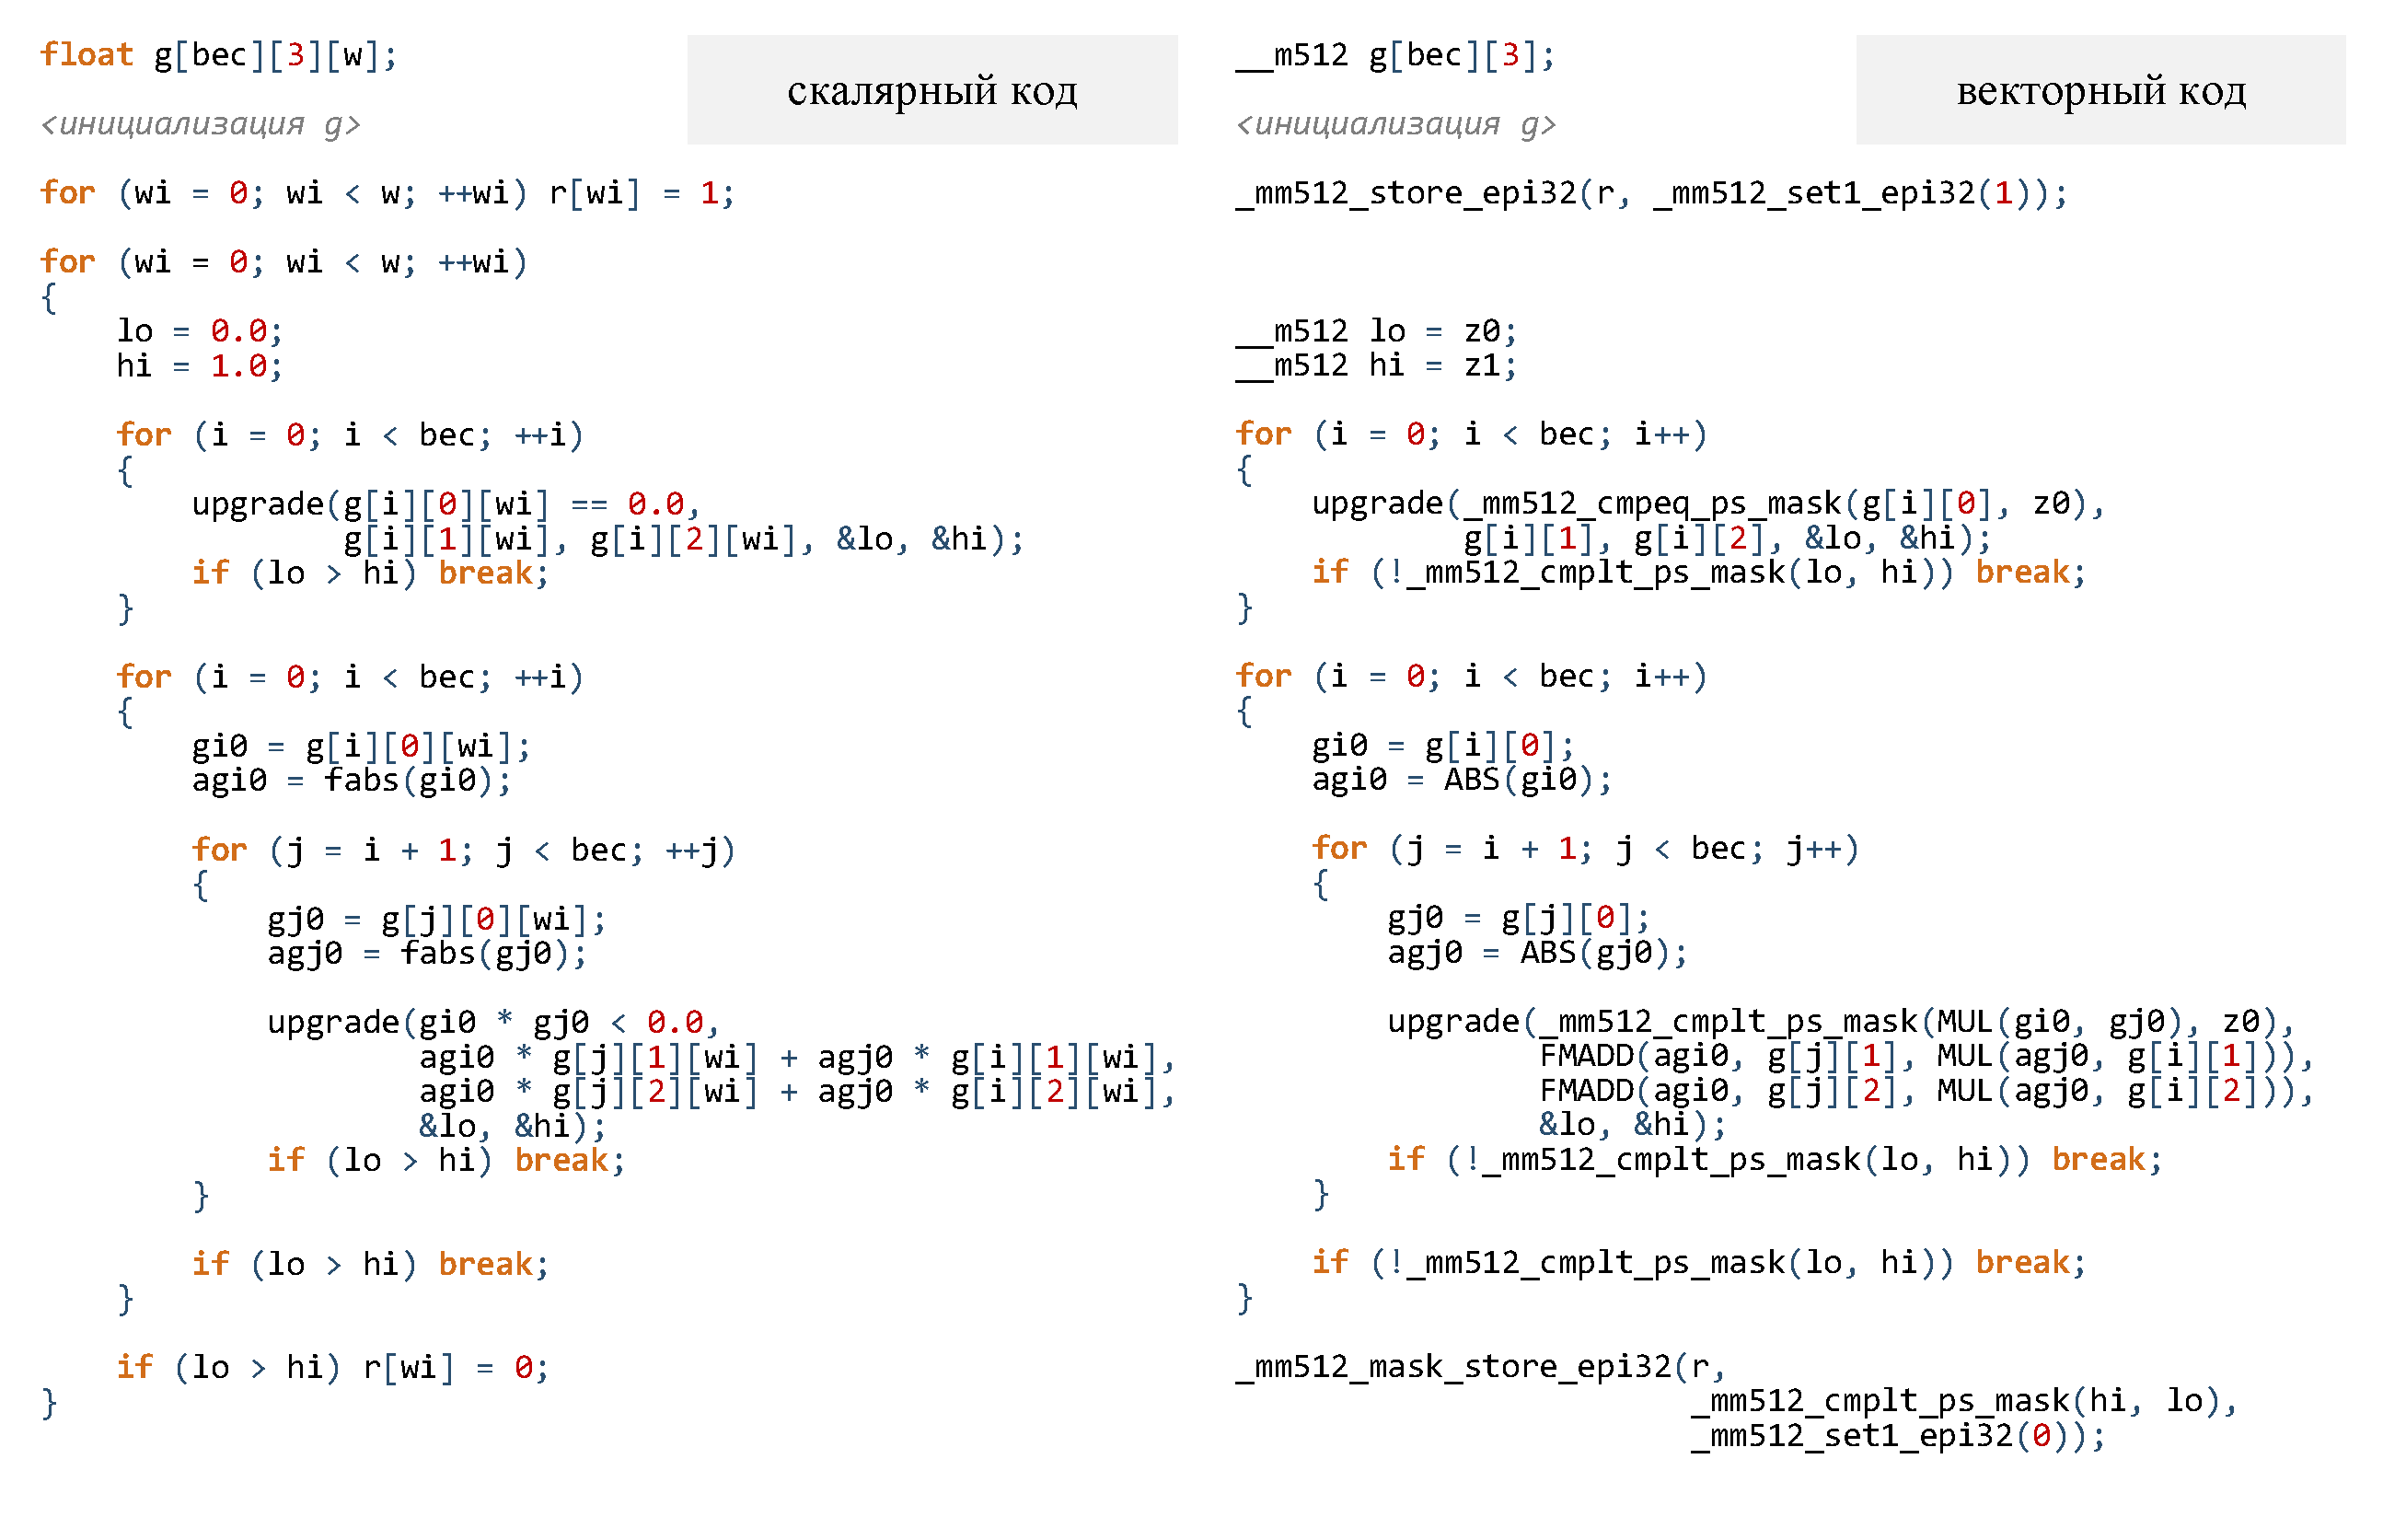
\includegraphics[width=1.0\textwidth]{fig/vec_mesh_intersect_final_scheme.pdf}
\singlespacing
\captionstyle{center}\caption{Схема перевода последовательного кода в векторный аналог для ядра функции \texttt{tri\_box\_intersect\_16}.}
\label{fig:text_1_mesh_intersect_scheme}
\end{figure}

Из рис.~\ref{fig:text_1_mesh_intersect_scheme} видно, что правильно составленный предикатный код (на рисунке слева) может быть довольно просто переведен в векторный аналог.
Для этого должны соблюдаться некоторые простые требования.
Во-первых, необходимо удалить все \texttt{else} ветки в условных операторах.
Этого можно добиться, например, путем расщепления оператора \texttt{if-else} на два противоположных условия.
После этого любое условие \texttt{if} легко трансформируется в предикат на весь блок кода, находящийся под условием.
Во-вторых, вызовы функции не должны находиться под предикатами.
Вместо этого в нашем случае скалярное условие вызова функции \texttt{upgrade} трансформировалось в аргумент функции, и после этого код легко поддается векторизации.
В остальном все вещественные скалярные инструкции были просто заменены на векторные аналоги.
Также была выполнена векторизация функции \texttt{upgrade} с помощью слияния всех веток выполнения под их предикатами, результирующий код этой функции представлен на листинге~\ref{lst:text_4_mesh_intersect_upgrade}.

\begin{singlespace}
\begin{lstlisting}[caption={Векторная реализация функции upgrade с пропагированным условием вызова внутрь функции.},label={lst:text_4_mesh_intersect_upgrade}]
void upgrade(__mmask16 m, __m512 f0, __m512 f1,
             __m512 *lo, __m512 *hi)
{
    __mmask16 c_f0z = _mm512_cmpeq_ps_mask(f0, z0);
    __mmask16 c_f0n = _mm512_cmplt_ps_mask(f0, z0);
    __mmask16 c_f0p = ~(c_f0z | c_f0n);
    __mmask16 c_f1p = _mm512_cmplt_ps_mask(z0, f1);
    __m512 k = _mm512_mask_div_ps(k, ~(m & c_f0z), f1, f0);
    k = SUB(z0, k);
    *lo = _mm512_mask_add_ps(*lo, m & c_f0z & c_f1p, *hi, z1);
    *hi = _mm512_mask_min_ps(*hi, m & c_f0p, *hi, k);
    *lo = _mm512_mask_max_ps(*lo, m & c_f0n, *lo, k);
}
\end{lstlisting}
\end{singlespace}

В результате преобразований был получен эффективный векторный код для поиска пересечений поверхностной и объемной расчетных сеток.
Функция определения пересечения пар ячеек продемонстрировала ускорение в 6,7 раза по сравнению с невекторизованной версией на микропроцессоре Intel Xeon Phi KNL\label{abbr:knl-10}.
Полный код доступен в \cite{iparGithub}.

% Векторизация римановского решателя.
\subsubsection{Внутренний цикл с непостоянным количеством итераций}\label{sec:text_4_vec_riemann}

В разделе~\ref{sec:text_4_vec_mesh_intersect} был рассмотрен пример векторизации плоского цикла, тело которого содержит циклы с постоянным количеством итераций.
При векторизации таких циклов условия перехода на следующую итерацию и выхода из внутреннего цикла переносятся в векторную версию кода без изменений.
Если количество итераций внутреннего цикла не является постоянным, то условия перехода на следующую итерацию и выхода из вложенного цикла зависят от номера итерации плоского цикла, то есть такие условия необходимо переводить в векторную форму с использованием векторных предикатов.
В этом разделе рассмотрим векторизацию такого программного контекста (тело плоского цикла содержит цикл с непостоянным количством итераций) на примере точного римановского решателя для задач газовой динамики \cite{Rybakov2019VecRiem1,Rybakov2019VecRiem2}.
Газодинамический решатель относится к программному контексту, в котором количество итераций внутреннего цикла меняется медленно с изменением номера итерации плоского цикла (то есть значение характеристики $\epsilon$ мало, а значение $e_{vec}^I$ близко к единице).

Рассматриваемая в этом разделе реализация римановского решателя находится в открытом доступе в составе библиотеки NUMERICA \cite{numericaGithub}.
Будем рассматривать одномерный случай для однокомпонентной среды, реализованный в виде чистой функции (функции без побочных эффектов, результат работы функции зависит только от значений входных параметров), которая по значениям плотности, скорости и давления газа слева $U_l = [d_l, u_l, p_l]$ и справа $U_r = [d_r, u_r, p_r]$ от разрыва, находит значения этих же величин на самом разрыве в нулевой момент времени после устранения перегородки $U = [d, u, p] = riem(U_l, U_r)$.
Трехмерный случай сводится к одномерному, полная реализация скалярной и векторизованной версии римановского решателя в трехмерном случае доступна в \cite{riemannvecGithub}.

\begin{figure}[ht]
\centering
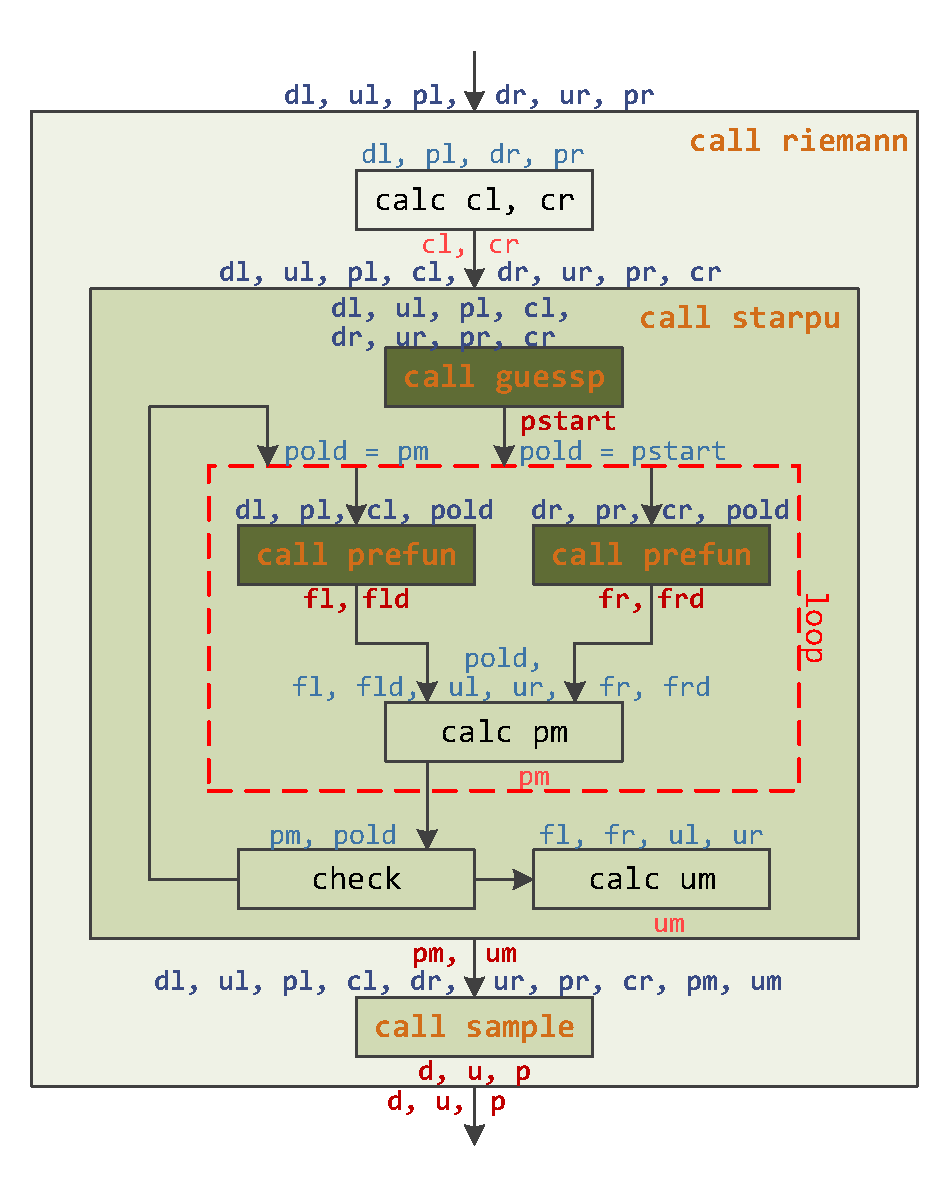
\includegraphics[width=0.5\textwidth]{fig/vec_riemann_functions.pdf}
\singlespacing
\captionstyle{center}\caption{Схема потока данных в римановском решателе}
\label{fig:text_4_vec_riem_functions}
\end{figure}

На Рис.~\ref{fig:text_4_vec_riem_functions} показана схема работы римановского решателя с обозначенными потоками данных и вызовами всех входящих в реализацию функций.
Функция \texttt{riemann} осуществляет вычисление скорости звука справа и слева, выполняет проверку на образование вакуума и последовательно вызывает функции \texttt{starpu} и \texttt{sample}.
Функция \texttt{starpu} вычисляет значения скорости и давления в среднем регионе между левой и правой волнами (star region), при этом функция содержит цикл с неизвестным количеством итераций для решения нелинейного уравнения итерационным методом Ньютона, внутри которого расположены вызовы других функций (\texttt{prefun}).
Функции \texttt{guessp} и \texttt{prefun} содержат только арифметические вычисления и простые условия.
Функция \texttt{sample} определяет окончательную конфигурацию разрыва путем вычисления множества условий и содержит очень разветвленное управление.

В процессе счета с помощью численных методов, базирующихся на римановском решателе, выполняется множество вызовов функции \texttt{riemann} с различными наборами входных данных.
Функция \texttt{riemann} является чистой, поэтому $w$ ее копий могут быть объединены в единый вызов с параметрами $\overline{U}_l = [\overline{d}_l, \overline{u}_l, \overline{p}_l]$, $\overline{U}_r = [\overline{d}_r, \overline{u}_r, \overline{p}_r]$, и результатом $\overline{U} = [\overline{d}, \overline{u}, \overline{p}] = riem(\overline{U}_l, \overline{U}_r)$.

Векторизация простой функции \texttt{prefun} с использованием простого слияния ветвей исполнения по условию с проверкой масок на пустоту, а также с объединением масок, уже рассматривалась в разделе \ref{sec:text_4_comb_mask_analyze}.
В этом разделе нас интересует функция \texttt{starpu}, которая содержит плоский цикл, тело которого содержит цикл с непостоянным количеством итераций.
Рассмотрим исходную реализацию скалярной версии функции \texttt{starpu}, представленную на листинге~\ref{lst:text_4_vec_riem_starpu}.

\begin{lstlisting}[caption={Оригинальная версия функции \texttt{starpu}.},label={lst:text_4_vec_riem_starpu}]
void starpu(float dl, float ul, float pl, float cl,
            float dr, float ur, float pr, float cr, float &p, float &u)
{
    const int nriter = 20;
    const float tolpre = 1.0e-6;
    float change, fl, fld, fr, frd, pold, pstart, udiff;

    guessp(dl, ul, pl, cl, dr, ur, pr, cr, pstart);
    pold = pstart;
    udiff = ur - ul;

    int i = 1;
    for ( ; i <= nriter; i++)
    {
        prefun(fl, fld, pold, dl, pl, cl);
        prefun(fr, frd, pold, dr, pr, cr);
        p = pold - (fl + fr + udiff) / (fld + frd);
        change = 2.0 * abs((p - pold) / (p + pold));

        if (change <= tolpre) break;
        if (p < 0.0) p = tolpre;

        pold = p;
    }

    if (i > nriter)
    {
        cout << "divergence in Newton-Raphson iteration" << endl;
        exit(1);
    }

    u = 0.5 * (ul + ur + fr - fl);
}
\end{lstlisting}

Цикл, расположенный в строках 13-24 кроме неизвестного количества итераций содержит также операторы передачи управления (\texttt{if}, \texttt{break}) и вызовы функций \texttt{prefun}, что также усложняет его векторизацию.
Перед выполнением векторизации этот цикл необходимо преобразовать в предикатную форму, в которой тело не должно содержать операций перехода.

\begin{lstlisting}[caption={Векторизованная версия функции \texttt{starpu}.},label={lst:text_4_vec_riem_starpu_vec}]
void starpu_16(__m512 dl, __m512 ul, __m512 pl, __m512 cl,
               __m512 dr, __m512 ur, __m512 pr, __m512 cr,
               __m512 *p, __m512 *u)
{
    ...
    two = SET1(2.0); tolpre = SET1(1.0e-6); tolpre2 = SET1(5.0e-7);
    udiff = SUB(ur, ul);

    guessp_16(dl, ul, pl, cl, dr, ur, pr, cr, &pold);

    // Start with full mask.
    m = 0xFFFF;

    for (; (iter <= nriter) && (m != 0x0); iter++)
    {
        prefun_16(&fl, &fld, pold, dl, pl, cl, m);
        prefun_16(&fr, &frd, pold, dr, pr, cr, m);
        *p = _mm512_mask_sub_ps(*p, m, pold,
                 _mm512_mask_div_ps(z, m,
                     ADD(ADD(fl, fr), udiff), ADD(fld, frd)));
        change = ABS(_mm512_mask_div_ps(z, m,
                         SUB(*p, pold), ADD(*p, pold)));
        cond_break = _mm512_mask_cmp_ps_mask(m, change,
                         tolpre2, _MM_CMPINT_LE);
        m &= ~cond_break;
        cond_neg = _mm512_mask_cmp_ps_mask(m, *p, z, _MM_CMPINT_LT);
        *p = _mm512_mask_mov_ps(*p, cond_neg, tolpre);
        pold = _mm512_mask_mov_ps(pold, m, *p);
    }

    if (iter > nriter)
    {
        cout << "divergence in Newton-Raphson iteration" << endl;
        exit(1);
    }

    *u = MUL(SET1(0.5), ADD(ADD(ul, ur), SUB(fr, fl)));
}
\end{lstlisting}

Запишем цикл в виде, при котором все инструкции цикла выполняются под своими предикатами, и выполнение цикла прерывается при условии обнуления всех предикатов \cite{Krzikalla2026Vec}.
При этом стоит заметить, что вызовы функций \texttt{prefun} также должны обладать соответствующими предикатами.
После преобразования тела цикла в предикатную форму, он может быть векторизован, после чего предикаты инструкций заменятся на векторные маски (именно в этом месте появляется дополнительный параметр векторизованной функции \texttt{prefun} в виде маски).
Результат векторизации функции \texttt{starpu} представлен на листинге~\ref{lst:text_4_vec_riem_starpu_vec}.
В строке 12 видна изначальная инициализация полной маски выполнения векторизованных итераций цикла.
По мере работы цикла маска истощается (строка 25), и при полном ее обнулении цикл завершает работу.

Для всех функций римановкого решателя была выполнена векторизация, полный программный код векторизованного решателя доступен в \cite{riemannvecGithub}.
Тестирование производительности выполнялось на массивах входных данных, собранных при решении стандартных тестовых задач: задача Сода, задача Лакса, задача о слабой ударной волне, задача Эйнфельдта, задача Вудворда-Колелла, задача Шу-Ошера и других \cite{Bulat2015VecRiemann}.
На диаграмме рис.~\ref{fig:text_4_vec_riemann_perf} показан эффект от применения различных оптимизаций к каждой из рассматриваемых функций, а также суммарное ускорение, полученное вследствие векторизации.

\begin{figure}
\centering
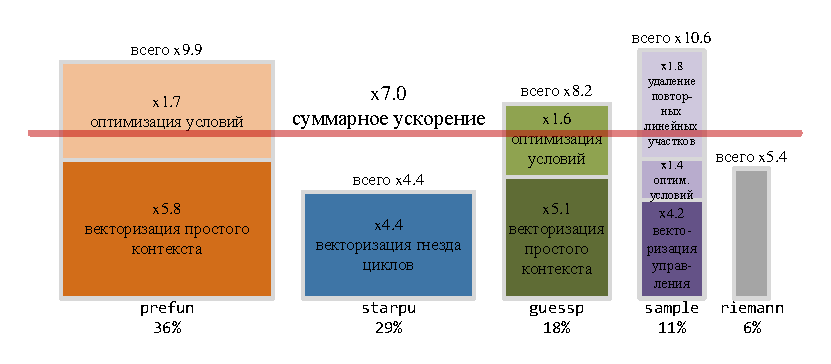
\includegraphics[width=1.0\textwidth]{fig/vec_riemann_perf.pdf}
\singlespacing
\captionstyle{center}\caption{Диаграмма ускорения отдельных функций и суммарного ускорения римановского решателя.}
\label{fig:text_4_vec_riemann_perf}
\end{figure}

Эффект от векторизации простого контекста варьируется в пределах от 5,1 до 5,8 раза (для функций \texttt{guessp} и \texttt{prefun}).
Также следует отметить существенный эффект от оптимизации условий (проверка на пустоту маски предикатов, под которой находится выполнение блока операций).
Это довольно простое преобразование, приводит к ускорению кода от 1,4 до 1,7 раз (для функций \texttt{sample} и \texttt{prefun}) в зависимости от того, насколько близкими являются условия с соседних итераций векторизуемого цикла.

% Векторизация циклов с нерегулярным количеством итераций.
\subsubsection{Внутренний цикл с нерегулярным количеством итераций}\label{sec:text_4_vec_irreg}

Рассмотренный в разделе \ref{sec:text_4_vec_riemann} программный контекст относится к моделированию физических процессов.
Для таких кодов характерно медленное изменение физических величин при переходе между ячейками.
Это свойство физических расчетных кодов позволяет эффективно выполнять векторизацию гнезд циклов с непостоянным количеством итераций.
В этом разделе рассмотрим принципиально другой тип контекста, в котором на двух соседних итерациях плоского цикла невозможно предсказать состояние условия, что приводит к возникновению гнезд циклов с нерегулярным количеством итераций \cite{Rybakov2019VecIrr,Shabanov2019VecSci}, что характеризуется значением $\epsilon$, сравнимым с $I_v$.

Рассмотрим реализацию сортировки Шелла, циклы в которой можно характерировать как циклы с нерегулярным количеством итераций.
Сортировка Шелла представляет собой расширение сортировки вставками, которое работает быстрее, так как позволяет на ранних этапах упорядочить далеко расположенные друг от друга элементы массива, это приводит к тому, что массив становится частично упорядоченным.
Во время сортировки Шелла выполняется последовательная сортировка подмассивов основного массива, являющихся срезами, при этом шаг среза постоянно уменьшается и на завершающем этапе выполняется обычная сортировка вставками (это соответствует срезу массива с шагом 1).
Выполнение сортировки срезов массива с большими шагами облегчает сортировку срезов с меньшими значениями шага, эффективность сортировки существенно зависит от выбранной последовательности шагов.
В литературе описано множество существующих последовательностей, из которых мы будем анализировать лишь некоторые, представленные в таблице~\ref{tbl:text_4_vec_irreg_steps}:

\begin{table}
\centering
\singlespacing
\captionstyle{center}\caption{Различные последовательности шагов, используемые в сортировке Шелла.}
\bigskip
\label{tbl:text_4_vec_irreg_steps}
\begin{tabular}{ | c | c | }
  \hline
  Последовательность & Формула \\ \hline\hline
  \makecell{Последовательность \\ Шелла}    & $k_1 = \lfloor \frac{N}{2} \rfloor, \ k_i = \lfloor \frac{k_{i-1}}{2} \rfloor, \ k_t = 1$ \\ \hline
  \makecell{Последовательность \\ Хиббарда} & $2^i - 1 \le N$, $i \in \mathbb{N}$ \\ \hline
  \makecell{Последовательность \\ Пратта}   & $2^i \cdot 3^j \le \frac{N}{2}$, $i \in \mathbb{N}$, $j \in \mathbb{N}$ \\ \hline
  \makecell{Последовательность \\ Седжвика} & $k_i = \begin{cases} 9 \cdot 2^i - 9 \cdot 2^{\frac{i}{2}} + 1, \ i = 2m, \ m \in \mathbb{Z}_{\ge 0} \\ 8 \cdot 2^i - 6 \cdot 2^{\frac{i + 1}{2}}, \ i = 2m + 1, \ m \in \mathbb{Z}_{\ge 0} \end{cases}$ \\ \hline
\end{tabular}
\end{table}

Реализация сортировки Шелла состоит из гнезда циклов, содержащего три цикла.
Внешний цикл выполняется по всем шагам из используемой последовательности шагов, начиная с максимального и заканчивая наименьшим шагом, равным единице.
Два внутренних цикла осуществляют сортировку всех подмассивов, являющихся срезами исходного массива с текущим шагом $k$ (листинг~\ref{lst:text_4_vec_irreg_shell}).

\begin{lstlisting}[caption={Реализация сортировки Шелла.},label={lst:text_4_vec_irreg_shell}]
void shell_sort(float* m, int n, int* ks, int k_ind)
{
    int i, j, k;

    for (k = ks[k_ind]; k > 0; k = ks[--k_ind])
    {
        for (i = k; i < n; i++)
        {
            float t = m[i];

            for (j = i; j >= k; j -= k)
            {
                if (t < m[j - k])
                {
                    m[j] = m[j - k];
                }
                else
                {
                    break;
                }
            }

            m[j] = t;
        }
    }
}
\end{lstlisting}

Рассмотрим возможности по векторизации сортировки Шелла для массива вещественных значений типа float (вектор AVX-512\label{abbr:avx-12} содержит 16 таких значений).
Самый вложенный цикл (цикл с счетчиком $j$, будем называть его просто внутренним) выполняет сортировку одного среза, состоящего из элементов массива, с расстоянием $k$ между соседними элементами.
Внутренний цикл не может быть векторизован без выполнения дополнительных модификаций кода, так как между записью элемента \texttt{m[j]} и чтением элемента \texttt{m[j - k]} существует межитерационная зависимость.
Две итерации среднего по вложенности цикла (цикла с индуктивной переменной $i$, будем называть его промежуточным) с номерами $i_1$ и $i_2$ не пересекаются по данным и могут быть выполнены параллельно при выполнении условия $|i_1 - i_2| < k$.
Выполним декомпозицию сортировки Шелла для того, чтобы можно было явно выделить ядро, поддающееся векторизации.

На рис.~\ref{fig:text_4_vec_irreg_code_decomp} представлена схема декомпозиции алгоритма сортировки Шелла, в котором явно выделены участки с разной максимально допустимой шириной векторизации, под которой мы будем понимать количество соседних итераций плоского цикла, независимых между собой.
Если максимально допустимая ширина векторизации оказывается ниже фактического значения, то вычисления необходимо производить с неполными масками, что приведет к деградации производительности).
Сначала выделен блок для шагов $k \ge 16$.
Для этих значений шагов можно параллельно выполнять 16 соседних итераций промежуточного цикла, при этом достигается максимальная плотность векторизации (показано зеленым цветом на схеме).

\begin{figure}[ht]
\centering
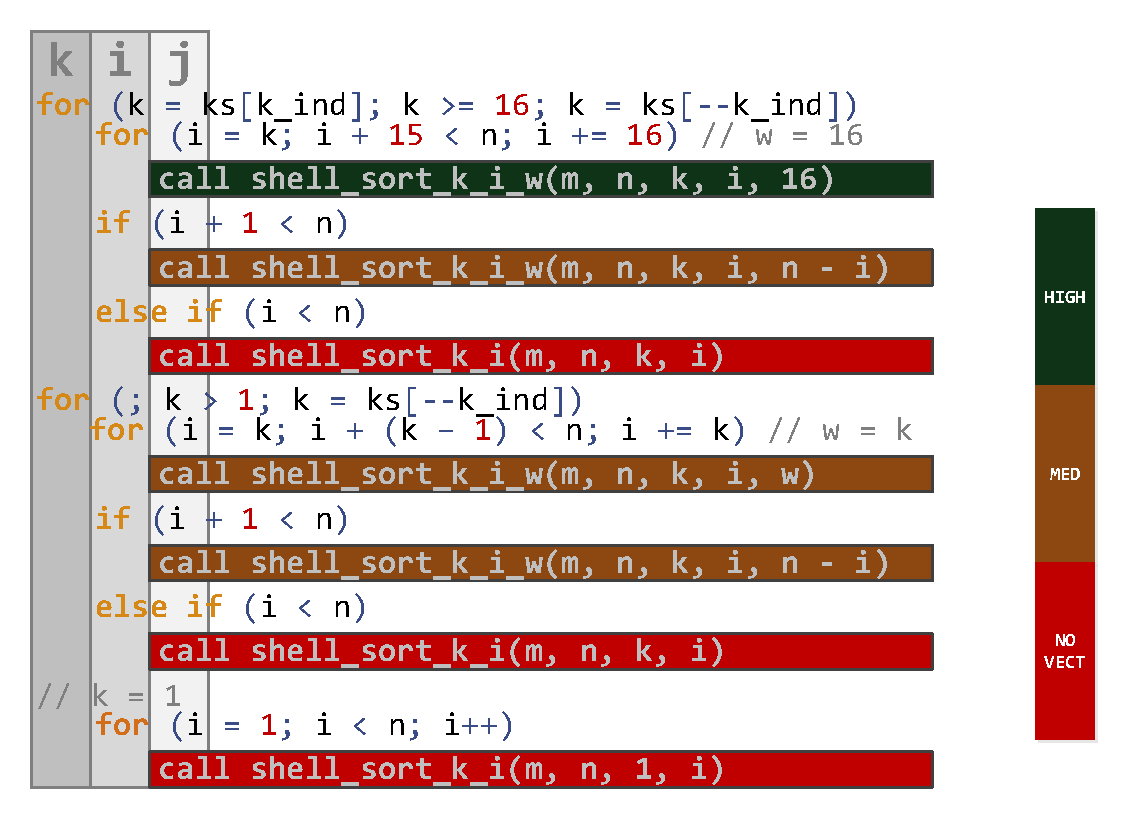
\includegraphics[width=0.7\textwidth]{fig/vec_shell_code_decomp.pdf}
\singlespacing
\captionstyle{center}\caption{Декомпозиция сортировки Шелла для выделения векторизуемых участков кода.}
\label{fig:text_4_vec_irreg_code_decomp}
\end{figure}

Все итерации промежуточного цикла разбиваются на группы по 16 соседних итераций и остаток, который векторизуется с шириной меньше 16 (показано желтым цветом, а в том случае, когда остаток состоит всего из одной итерации, то векторизация не требуется, что показано красным цветом на схеме).
Далее рассматривается блок значений шагов $1 < k < 16$.
При этих значениях максимально допустимая ширина векторизации всегда меньше 16, к тому же, как и в предыдущем блоке, возможно появление невекторизуемого остатка.

В последнюю очередь рассматривается невекторизуемая финальная сортировка вставками для $k = 1$.
Наличие участков кода с шириной векторизации менее 16 приводит к неоптимальному результирующему коду, однако есть более опасная причина низкой эффективности векторизации.

Функция \texttt{shell\_sort\_k\_i\_w}, появившаяся после декомпозиции алгоритма сортировки Шелла, содержит реализацию сортировки $w$ соседних срезов массива, взятых с шагом $k$.
При этом количество итераций внутреннего цикла этой функции является неизвестным.
Более того, количество итераций внутреннего цикла при сортировке одного среза никак не связано с количеством итераций внутреннего цикла при сортировке соседнего среза.
Это является существенной проблемой при попытке объединить код сортировки соседних срезов, используя векторные инструкции.

Для такого объединения необходимо переписать код сортировки среза в предикатной форме, после чего заменить все инструкции векторными аналогами, а предикаты –- векторными масками (см. рис.~\ref{fig:text_4_vec_irreg_shell_cfg}).
При этом если до векторизации внутренний цикл завершал работу при обращении предиката в false, то после векторизации внутренний цикл завершит работу, только если все элементы соответствующей векторной маски обнулятся.
Таким образом, количество итераций векторизованного внутреннего цикла равно максимальному количеству итераций всех объединяемых $w$ циклов.

\begin{figure}[ht]
\centering
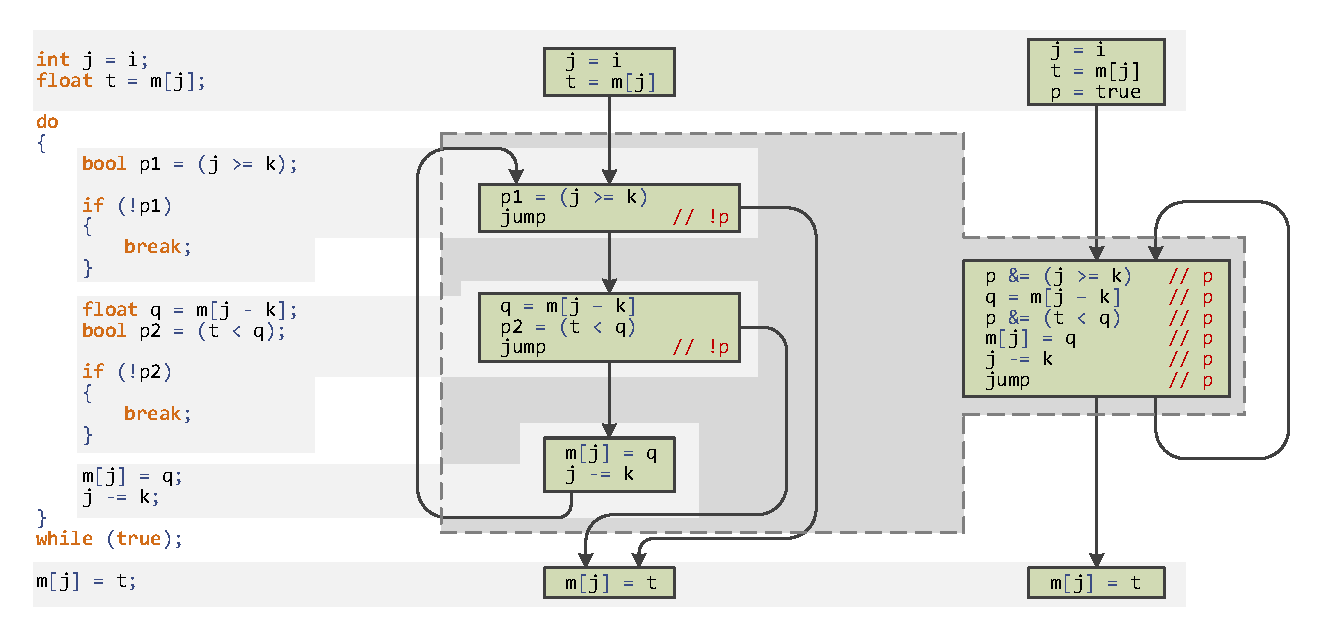
\includegraphics[width=1.0\textwidth]{fig/vec_shell_cfg.pdf}
\singlespacing
\captionstyle{center}\caption{Схема перевода тела внутреннего цикла сортировки Шелла в предикатную форму.}
\label{fig:text_4_vec_irreg_shell_cfg}
\end{figure}

Если значения количества итераций соседних объединяемых циклов различаются сильно (а для сортировки Шелла это утверждение верно), то мы получаем потерю эффективности векторизации из за низкой плотности масок векторных инструкций (то есть малый процент элементов векторов на самом деле обрабатывается при выполнении векторной операции).
Такой негативный эффект при векторизации гнезд циклов характерен для дискретных задач, в том числе для задач сортировки, поиска, комбинаторного перебора с отсечением ветвей и других.
Для задач численного моделирования физических процессов ситуация обратная -- для соседних итераций плоского цикла профиль исполнения отдельных участков программного кода тела цикла меняется не сильно при небольших изменениях входных данных.
Векторизованная версия ядра сортировки Шелла представлена на листинге~\ref{lst:text_4_vec_irreg_shell_vec} (полный код доступен в \cite{iparGithub}):

\begin{lstlisting}[caption={Векторизованный вариант ядра сортировки Шелла.},label={lst:text_4_vec_irreg_shell_vec}]
void shell_sort_k_i_w(float *m, int n, int k, int i, int w)
{
    int j = i;
    __mmask16 ini_mask = ((unsigned int)0xFFFF) >> (16 - w);
    __mmask16 mask = ini_mask;
    __m512i ind_j = _mm512_add_epi32(_mm512_set1_epi32(i),
                                     ind_straight);
    __m512 t, q;

    t = _mm512_mask_load_ps(t, mask, &m[j]);

    do
    {
        mask = mask & _mm512_mask_cmp_epi32_mask(mask, ind_j, ind_k,
                                                 _MM_CMPINT_GE);
        q = _mm512_mask_load_ps(q, mask, &m[j - k]);
        mask = mask & _mm512_mask_cmp_ps_mask(mask, t, q,
                                              _MM_CMPINT_LT);
        _mm512_mask_store_ps(&m[j], mask, q);
        ind_j = _mm512_mask_sub_epi32(ind_j, mask, ind_j, ind_k);
        j -= k;
    }
    while (mask != 0x0);

    _mm512_mask_i32scatter_ps(m, ini_mask, ind_j, t, _MM_SCALE_4);
}
\end{lstlisting}

Также стоит обратить внимание на появившуюся в векторном коде операцию scatter (листинг~\ref{lst:text_4_vec_irreg_shell_vec}, строка 25) множественной записи данных в память с произвольными смещениями относительно базового адреса.
Эта команда появилась как векторный аналог операции записи в память из оригинального кода (листинг~\ref{lst:text_4_vec_irreg_shell}, строка 23) ввиду той же причины –- нерегулярности количества итераций внутреннего цикла.
Команда scatter является медленной, что также является причиной снижения эффективности векторизации.

Кроме обозначенной команды scatter в векторизованном коде присутствуют другие команды обращения в память (листинг~\ref{lst:text_4_vec_irreg_shell_vec}, строки 10, 16, 19).
Это масочные команды чтения и записи по последовательным адресам, реализованные интринсиками \texttt{\_mm512\_mask\_load\_ps} и \texttt{\_mm512\_mask\_store\_ps}, которые раскрываются в операции невыровненного обращения в память vmovups.
Выровненные операции обращения в память использовать нельзя, так как в общем случае адреса обращения в этих командах не являются кратными размеру вектора.
В микропроцессорах Intel Xeon Phi KNL и Intel Xeon Skylake скорость обращения в память команд vmovaps не отличается от скорости обращения vmovups при условии выровненного обращения, поэтому компилятор icc вовсе не генерирует инструкции vmovaps \cite{MOVUPSintel}.
Таким образом, при невыполнении условия выровненности адресов вместо аварийного завершения мы получаем снижение производительности программы, однако это снижение не сравнимо с медленной работой инструкций gather и scatter.

\begin{figure}[ht]
\centering
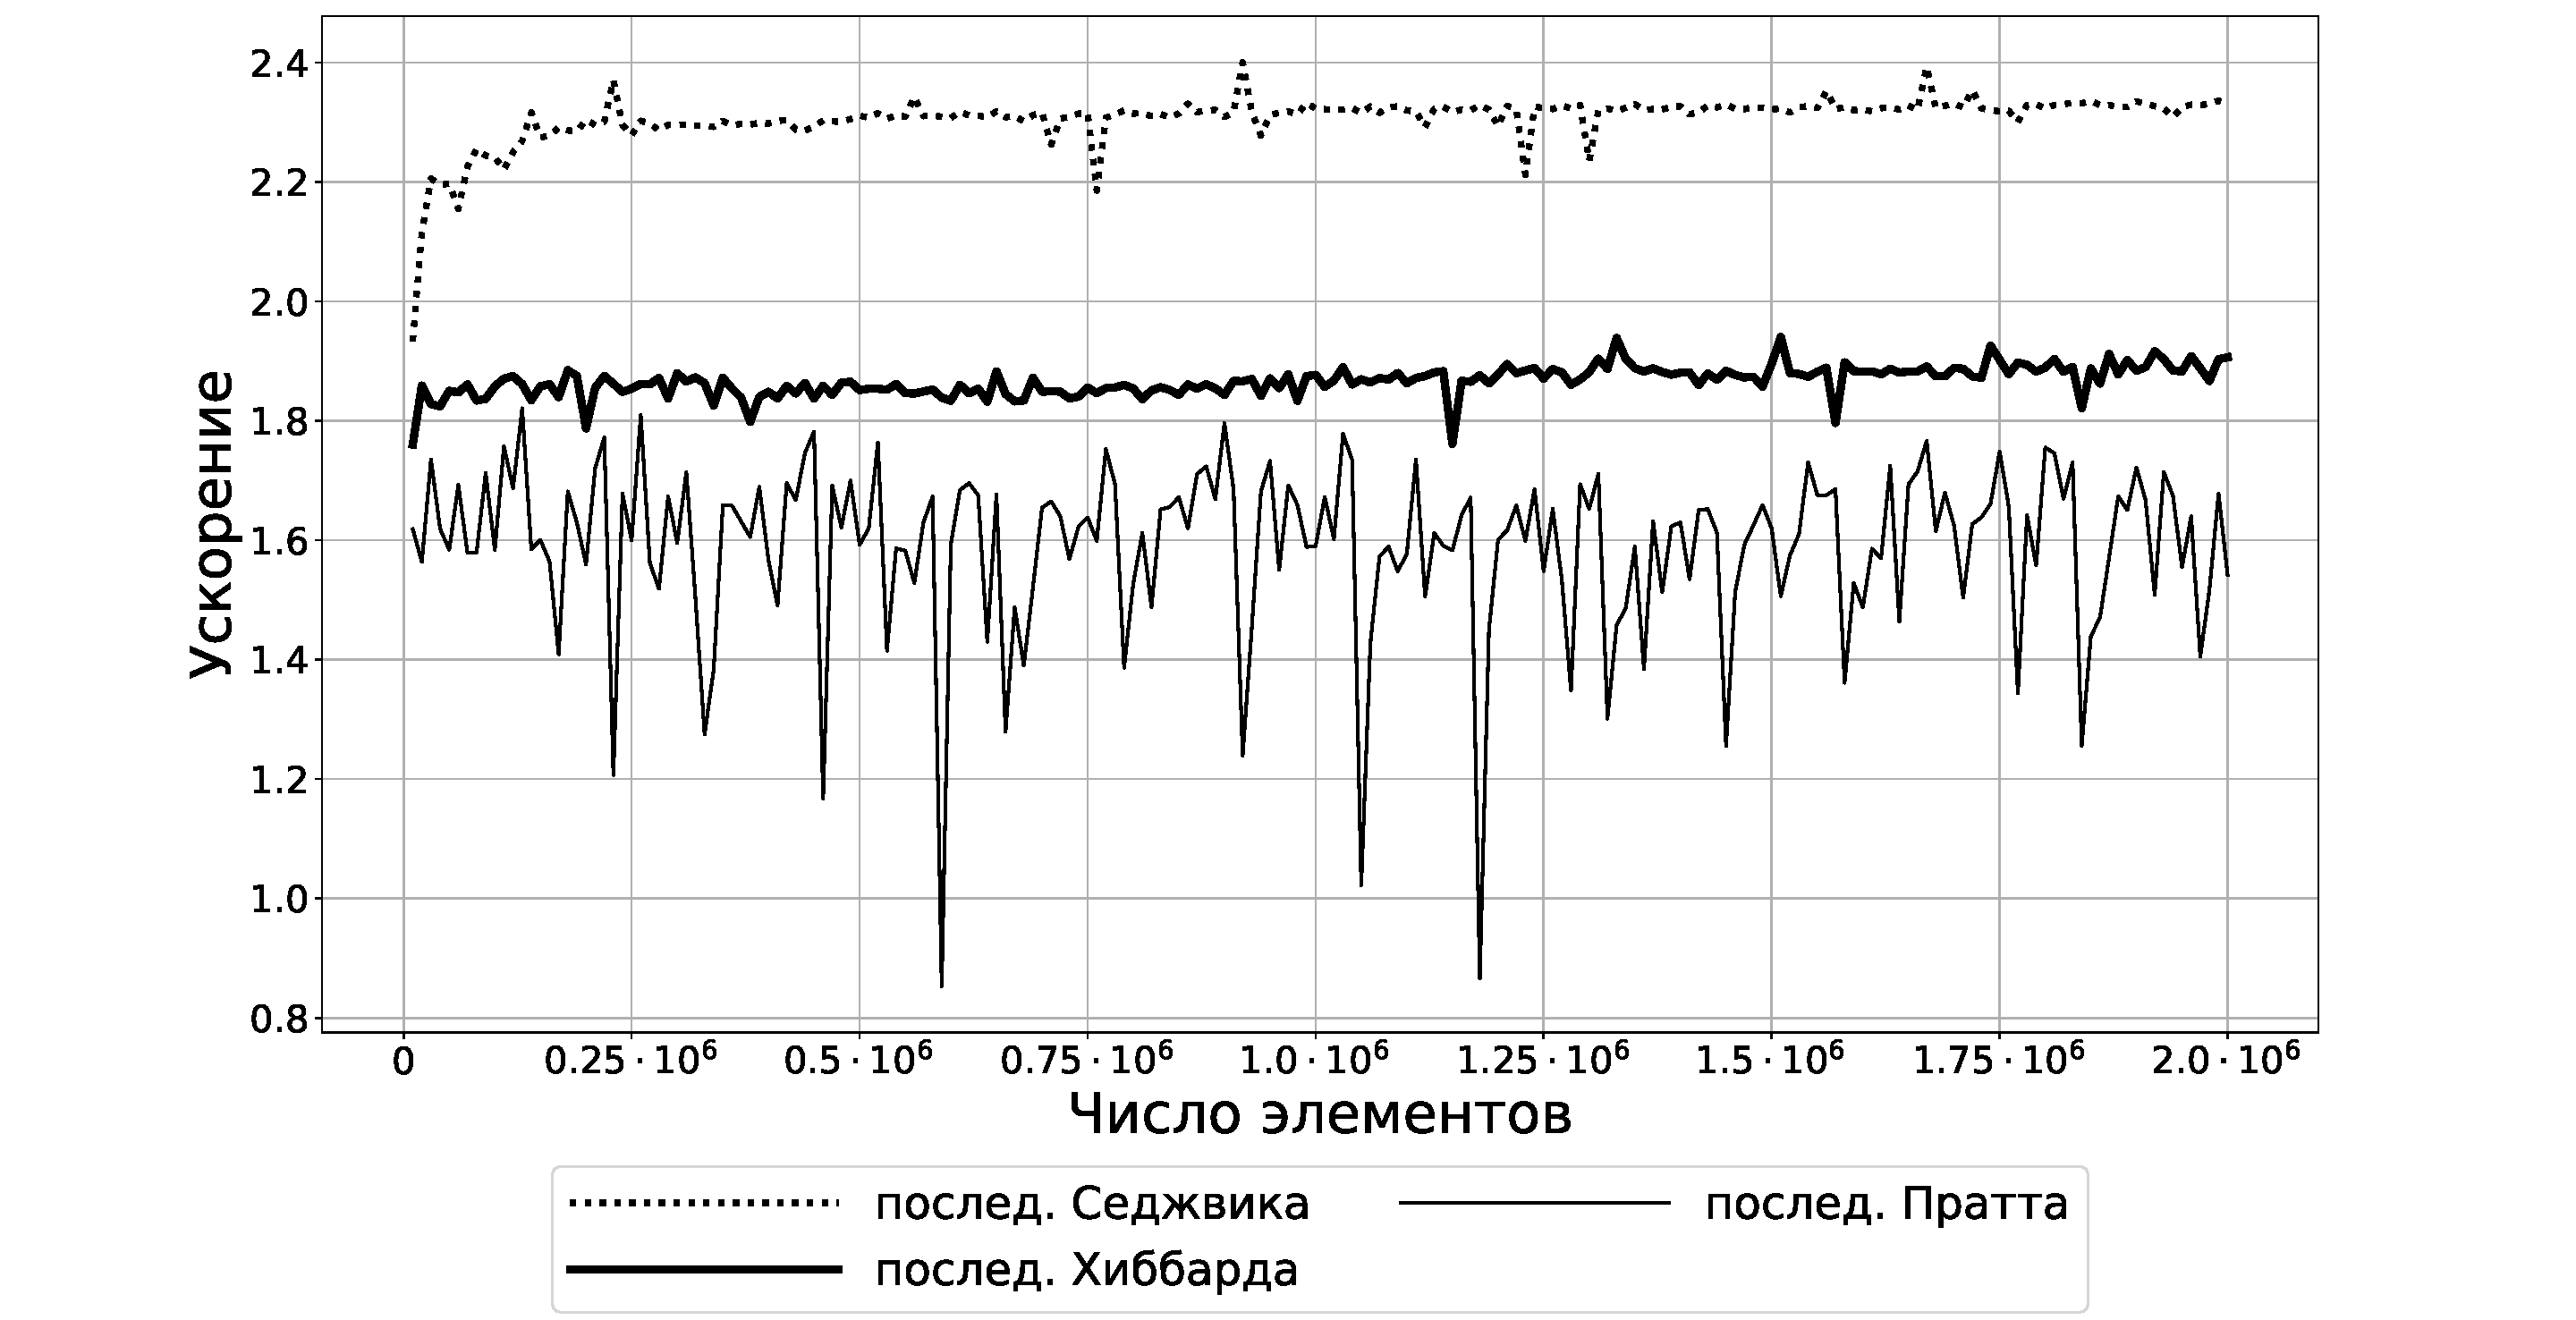
\includegraphics[width=1.0\textwidth]{fig/vec_shell_experimental_eff.pdf}
\singlespacing
\captionstyle{center}\caption{Ускорение векторизованной версии сортировки Шелла для различных последовательностей шагов.}
\label{fig:text_4_vec_irreg_eff}
\end{figure}

Для проведения экспериментов по замеру ускорения были использованы две версии исходного кода: неоптимизированная функция сортировки и реализованная с помощью функций-инстринсиков.
Обе версии сортировки были собраны компилятором icc с уровнем оптимизаии -O3.
Тестовые запуски и замер времени исполнения выполнялись на микропроцессоре Intel Xeon Phi KNL\label{abbr:knl-11}.

На рис.~\ref{fig:text_4_vec_irreg_eff} представлены результаты экспериментальных запусков для замеров ускорения векторизованного кода для последовательностей шагов Шелла, Хиббарда и Сэджвика.
Результаты показали, что ускорение сортировки Шелла редко превышает отметку 2.

%\begin{figure}[ht]
%\centering
%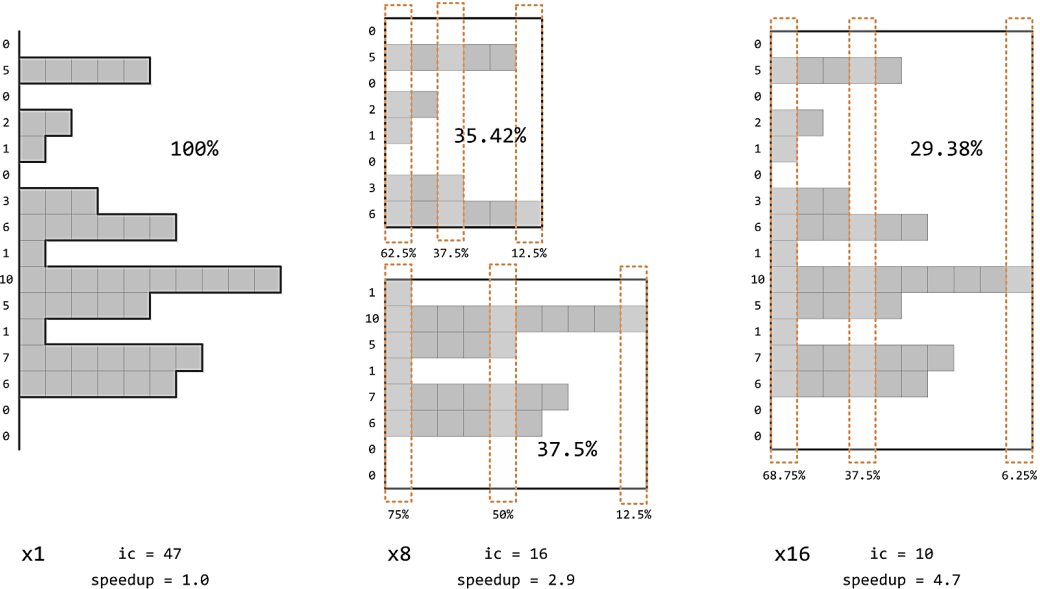
\includegraphics[width=0.8\textwidth]{./pics/text_4_vec_irreg/pack.png}
%\singlespacing
%\captionstyle{center}\caption{Иллюстрация потери производительности для вложенного цикла с нерегуярным количеством итераций.}
%\label{fig:text_4_vec_irreg_pack}
%\end{figure}

\subsubsection{Внутренний цикл с нерегулярным количеством итераций в целочисленном программном контексте}\label{sec:text_4_integer}

В разделах~\ref{sec:text_4_vec_riemann} и \ref{sec:text_4_vec_irreg} была рассмотрена векторизация плоских циклов с телом в виде циклов с непостоянным количеством итераций при работе с вещественными числами.
В этом разделе будет рассмотрен пример векторизации для целочисленного программного контекста -- программного код, в котором преобладают целочисленные вычисления, а также ведется работа с дискретными структурами данных.
Работа целочисленным программным контекстом отличается, как правило, наличием циклов с нерегулярным количеством итераций, а также нерегулярными обращениями в память в косвенностью и частыми промахами в кеш.
В качестве примера целочисленного программного контекста будем рассматривать алгоритм декомпозиции графа из раздела~\ref{sec:text_2_genetic}.

Алгоритм пузырькового роста из раздела~\ref{sec:text_2_genetic}, используемый в генетическом алгоритме декомпозиции графа, требует эффективной реализации, так как в составе генетического алгоритма он должен исполняться многократно для одного и того же графа, но с разными настройками декомпозиции, закодированными в генотипе декомпозиции.
Этот алгоритм работает с целочисленным программным контекстом и может быть векторизован с помощью векторных операций над упакованными целыми числами.

Рассмотрим возможности по ускорению алгоритма пузырьковго роста с помощью векторизации.
Пусть на вход в алгоритм, реализованный на языке C++, подается граф, информация о его ребрах записана в массиве \texttt{inc}, где \texttt{inc[i]} –- массив номеров всех вершин, смежных с вершиной $i$.
Номера доменов, к которым относятся конкретные вершины хранятся в массиве \texttt{domains}.
В алгоритме пузырькового роста домены наращиваются последовательно с помощью алгоритма обхода графа в ширину, начиная от инициирующих вершин.
Структура \texttt{q} -- массив очередей вершин, ожидающих попадания в домены, в начале работы алгоритма очередь \texttt{q[i]} содержит только одну инициирующую вершину $i$-го домена.
В качестве масссива и очереди используются структуры STL vector и queue соответственно.
Пусть требуется выполнить декомпозицию (или раскраску вершин графа) на \texttt{domains\_count} доменов.
Тогда простейшая реализация алгоритма пузырькового роста доменов от инициирующих вершин может иметь следующий вид (см. листинг~\ref{lst:text_4_vec_integer}):

\begin{lstlisting}[caption={Реализация алгоритма пузырькового роста доменов.},label={lst:text_4_vec_integer}]
while (is_q)
{
    is_q = false;

    for (size_t c = 0; c < domains_count; ++c)
    {
        if (q[c].empty()) continue;

        is_q = true;
        n = q[c].front();
        q[c].pop();

        if (domains[n] == -1)
        {
            domains[n] = c;
            for (auto ngh : inc[n]) q[c].push(ngh);
        }
    }
}
\end{lstlisting}

Реализация алгоритма представляет собой гнездо из 3 циклов.
Внешний цикл выполняется до тех пор, пока найдется хотя бы одна непустая очередь домена.
Средний цикл выполнятся по номерам доменов.
Для каждого домена берется первая необработанная вершина из соответствующей очереди, и если она еще не отнесена ни к одному домену, то она заносится в текущий домен, а все ее соседи отправляются в очередь.
Внутренний цикл -- цикл по всем соседям только что обработанной вершины, которые должны быть занесены в очередь.
Будем выполнять векторизацию представленного кода по среднему циклу, и для простоты анализа приведем реализацию для фиксированного значения \texttt{domains\_count = 16} (это позволит избавиться от среднего цикла, и заменить его набором отдельных векторных операций).

Для выполнения векторизации вначале необходимо избавиться от STL\label{abbr:stl-1} структур vector и queue, так как они имеют свою внутреннюю реализацию, и векторизация операций по работе с ними невозможна.
Вместо структуры \texttt{vector<int>} будем хранить информацию о списке соседних вершин просто в массиве, 0-м элементом которого будет его размер.
Очередь queue также будет имитировать с помощью массива и индексов \texttt{front} и \texttt{back}, указывающих на первый и последний элементы очереди соответственно.
Тогда операция \texttt{push(v)} будет соответствовать записи в массив по индексу \texttt{back} с его продвижением, а операция \texttt{pop} будет соответствовать просто продвижению индекса \texttt{front}.
Очередь пуста если ее индекс \texttt{front} больше индекса \texttt{back}.

\begin{figure}[ht]
\centering
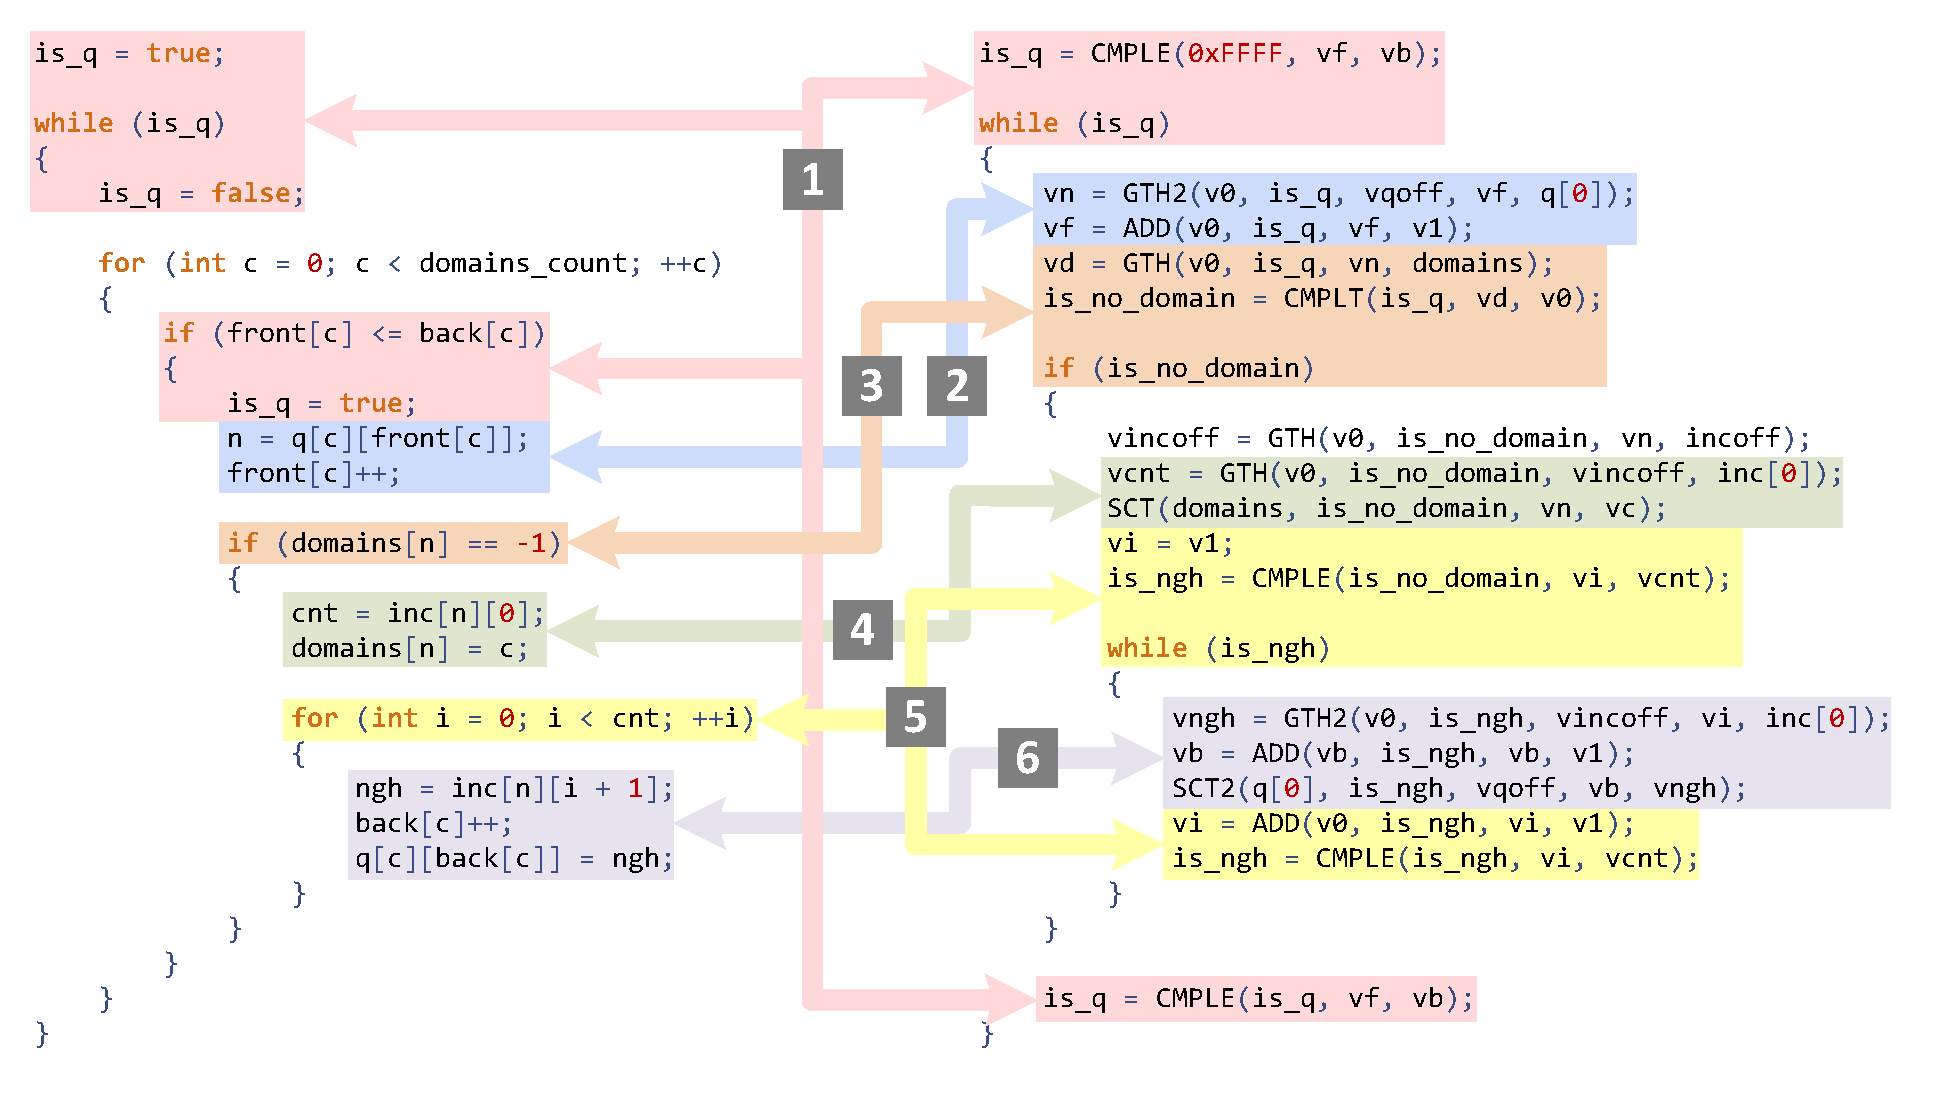
\includegraphics[width=0.90\textwidth]{fig/vec_genetic_code.pdf}
\singlespacing
\captionstyle{center}\caption{Векторизация программного кода алгоритма пузырькового роста путем замены скалярных инструкций векторными аналогами.}
\label{fig:text_4_vec_integer_code}
\end{figure}

На рис.~\ref{fig:text_4_vec_integer_code} представлены скалярная и векторная версии программного кода реализации алгоритма пузырькового роста.
Полная версия исходного кода доступна в \cite{comboptGithub}.
В векторной версии \texttt{ADD} обозначает функцию-интринсик \texttt{\_mm512\_mask\_add\_epi32}, \texttt{GTH} и \texttt{SCT} -- аналогично представляют собой краткие имена для интринсиков операций gather и scatter.
Обозначения \texttt{GTH2} и \texttt{SCT2} -- это те же операции \texttt{GTH} и \texttt{SCT}, только использующие сразу два смещения от базового адреса).
Через \texttt{CMPLE}, \texttt{CMPLT} обозначены вызовы функции-интринсика \texttt{\_mm512\_mask\_cmp\_epi32\_mask} с параметрами сравнения \texttt{\_MM\_CMPINT\_LE} и \texttt{\_MM\_CMPINT\_LT} соответственно.
На рис.~\ref{fig:text_4_vec_integer_code} цифрой <<1>> обозначена векторизация условия продолжения выполнения внешнего цикла (цикл завершает работу, если все очереди доменов пусты).
Цифрой <<2>> обозначена векторизация извлечения следующей вершины из каждой очереди.
Цифрой <<3>> обозначена проверка принадлежности извлеченных вершин к какому-либо домену (в векторной версии формируется маска \texttt{is\_no\_domain} -- маска с номерами доменов, в которые добавляется новая вершина).
Цифрой <<4>> обозначена векторизация помещения рассматриваемой вершины в текущий домен и получение количества ее соседей. 
Цифра <<5>> -- обработка всех соседей только что помещенной в домен вершины, и цифра <<6>> -- добавление этих соседей в соответствующие очереди.

Для оценки эффективности проведенной векторизации были произведены запуски на дуальных графах поверхностных прямоугольных расчетных сеток со стороной от 20 до 2000 ячеек (то есть на графах с количеством вершин от 400 до 4 млн).
Замеры ускорения выполнялись на микропроцессоре Intel Xeon Phi KNL\label{abbr:knl-12}, результаты представлены на рис.~\ref{fig:text_4_vec_integer_sp}, для удобства приведен также график сглаженного показателя ускорения.

\begin{figure}[ht]
\centering
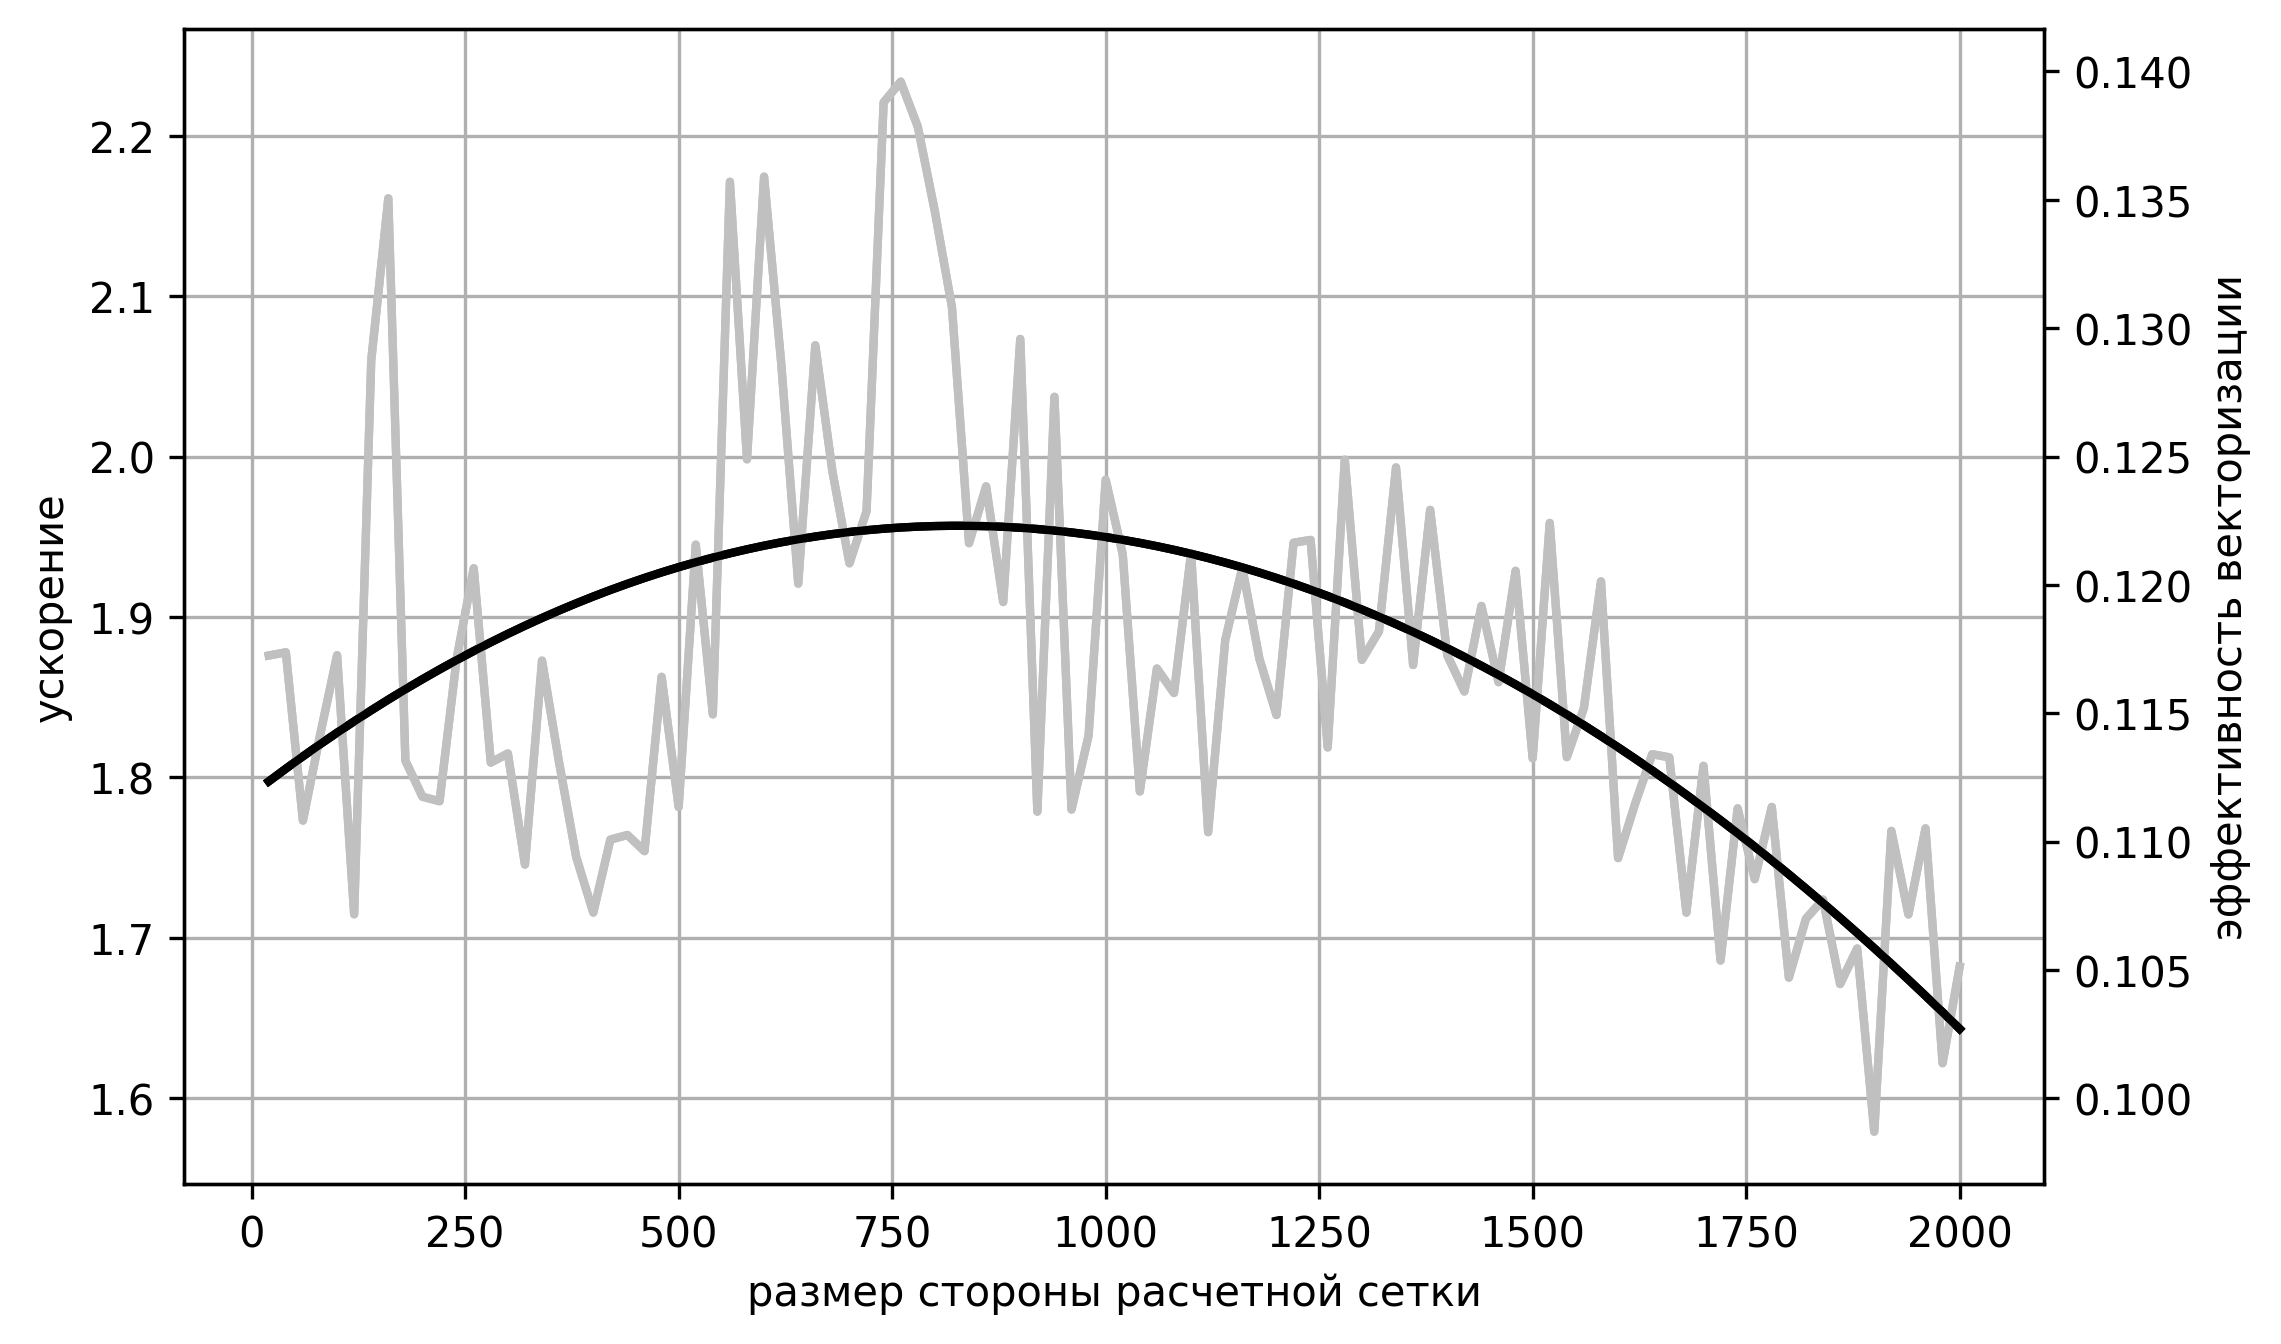
\includegraphics[width=0.7\textwidth]{fig/vec_genetic_chart_speedup_rus.png}
\singlespacing
\captionstyle{center}\caption{Ускорение и эффективность векторизации алгоритма пузырькового роста в зависимости от размера стороны расчетной сетки.}
\label{fig:text_4_vec_integer_sp}
\end{figure}

Замеры ускорения продемонстрировали ускорение в диапазоне 1,7-2,2 раза для рассматриваемых графов с количеством ячеек от 400 до 4 млн.
Анализируя график сглаженного показателя ускорения, можно отметить, что максимум наблюдается при размере стороны расчетной сетки в районе 750 и равен примерно 1,95.
Снижение ускорения при уменьшении стороны расчетной сетки связано с увеличение количества конфликтов при обработке следующих вершин из очередей доменов.
Снижение ускорения при увеличении стороны расчетной сетки связано с увеличением разброса смещений при выполнении операций gather/scatter, что приводит к промахам в кэш-память.
Продемонстрированные невысокие результаты ускорения объясняются прежде всего нерегулярным количеством итераций циклов в гнезде, а также обилием операций множественного обращения в память gather/scatter.

%---------------------------------------------------------------------------------------------------
% Выводы.

\subsection{Выводы из главы}

\begin{figure}[ht]
\centering
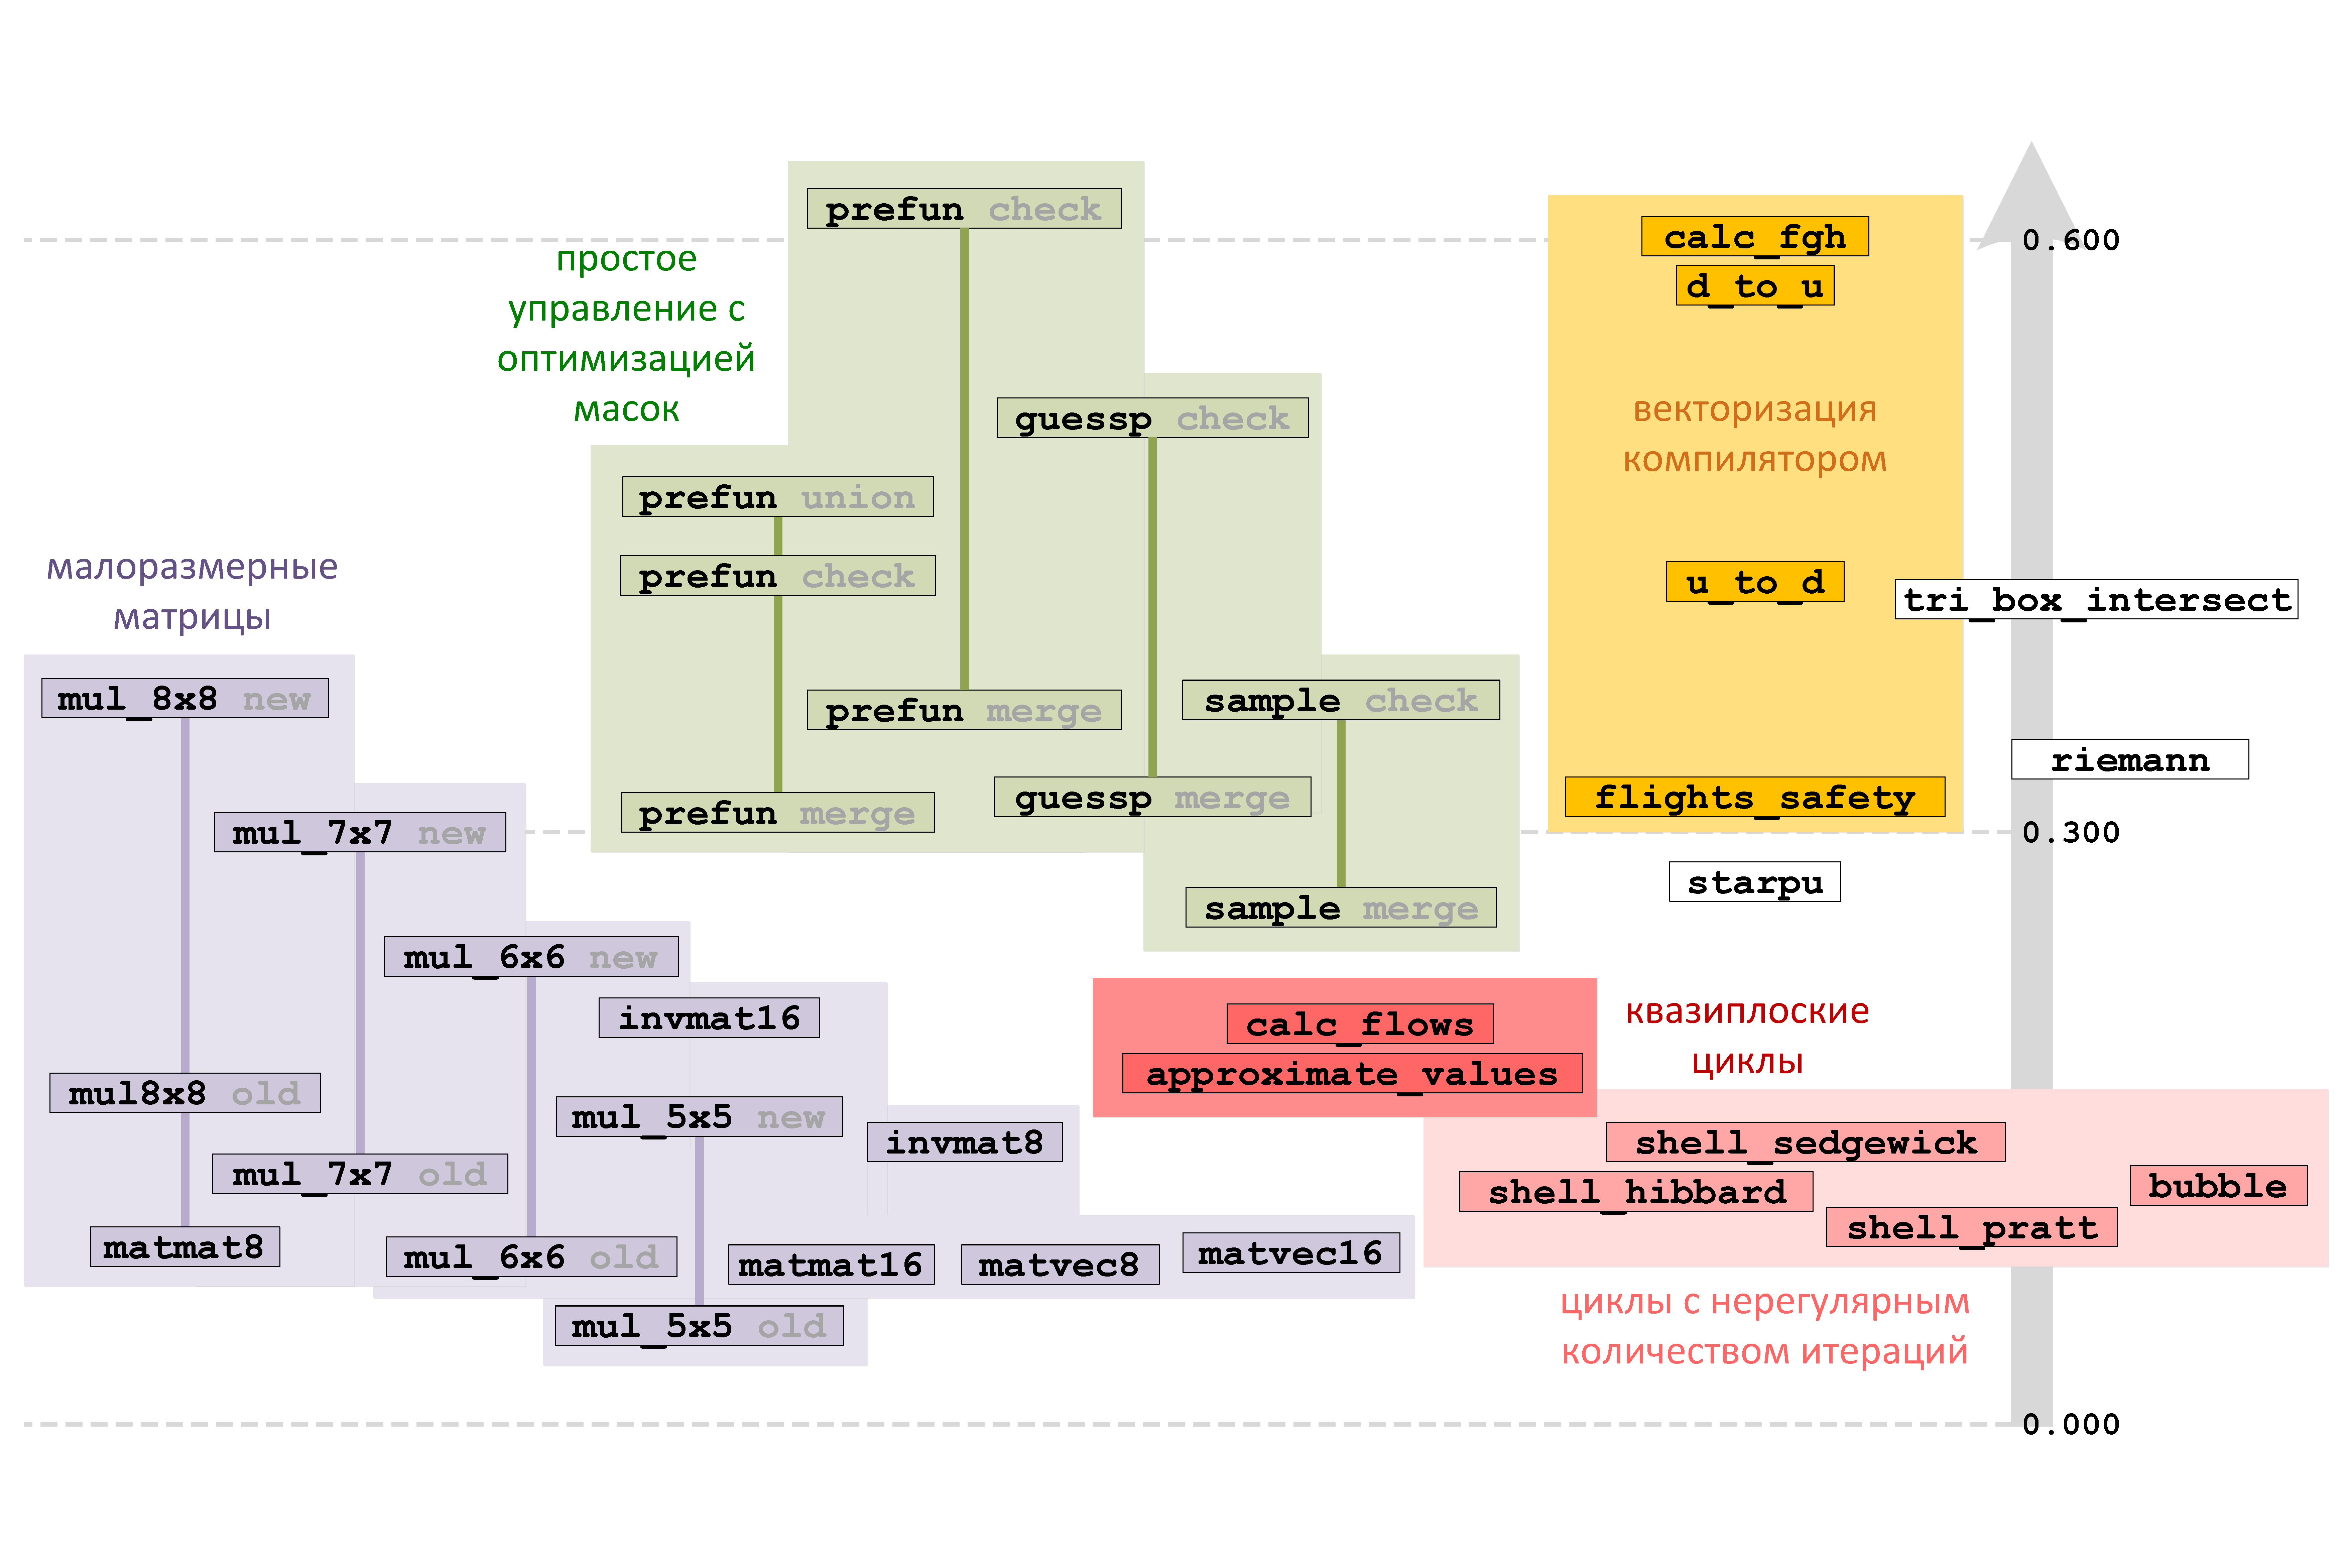
\includegraphics[width=1.0\textwidth]{fig/vec_map_cut.pdf}
\singlespacing
\captionstyle{center}\caption{Карта эффективности векторизации.}
\label{fig:text_4_fin_map}
\end{figure}

Векторизация является важной низкоуровневой оптимизацией программного кода, с помощью которой можно достичь кратного ускорения суперкомпьютерных приложений.
Все основные современные микропроцессорные архитектуры поддерживают векторные вычисления, причем наблюдается тенденция на увеличение размера вектора (на сегодняшний день максимальная длина равна 512 битам, но уже сейчас логически эта длина не ограничена, учитывая наборы векторных инструкций с переменной длиной вектора).

Сейчас наиболее перспективным набором векторных инструкций является набор AVX-512\label{abbr:avx-13}, так как в нем поддержана возможность выборочной обработки элементов векторов с помощью векторных масок.
Эта уникальная возможность позволяет векторизовать сложный программный контекст, содержащий команды передачи управления, гнезда циклов и вызовы функций.

В этой главе были рассмотрены и предложены новые методы векторизации программного кода.
На рис.~\ref{fig:text_4_fin_map} приведена карта сравнения программного контекста различного вида по эффективности векторизации $e_{vec}$.
На этом рисунке схожие по свойствам тестовые примеры объединены в одной цветовой гамме.
Многие из представленных тестовых примеров векторизации программного кода были использованы при численном решении задач обледенения и газовой динамики.

В разделах \ref{sec:text_4_small_matr}, и \ref{sec:text_4_spec_matr} продемонстрированы подходы к векторизации матричных операций малой размерности.
При выполнении векторизации программного кода необходимо уметь находить наборы однотипных операций для объединения их в векторные операции над векторными наборами данных.
При этом полнота использования элементов векторных данных в вычислениях, выраженная в высокой плотности векторных масок, напрямую влияет на эффективность векторизации (см. риc.~\ref{fig:text_4_fin_map}, малоразмерные матрицы).

В разделе \ref{sec:text_4_flat} введено понятие плоского цикла, с помощью которого предпринимается попытка унифицировать процесс объединения однотипных операций в векторные инструкции путем записи тела плоского цикла в предикатной форме с последущей векторизацией с помощью замены скалярных операций векторными аналогами.
Можно констатировать, что плоский цикл может быть векторизован при практически произвольном виде его тела (тело может содержать сложное управления, гнезда циклов, вызовы функций).

В разделе \ref{sec:text_4_ibm} приведено описание подхода, как вычисления могут быть представлены в виде композиции плоских циклов с относительно простым телом, после чего успешно векторизованы оптимизирующим компилятором в автоматическом режиме (см. рис.~\ref{fig:text_4_fin_map}, \texttt{calc\_fgh}, \texttt{calc\_d\_to\_u}, \texttt{calc\_u\_to\_d}).
При этом рассматривается предпочтительный способ организации хранения данных в виде <<набора массивов>> и оптимизация расщепления гнезда циклов по условию для уменьшения количества операций передачи управления внутри плоского цикла.
Отмечено, что цикл, не являющийся в полной мере плоским (квазиплоский цикл), также может быть успешно векторизован, но с некоторой потерей производительности (см. рис.~\ref{fig:text_4_fin_map}, \texttt{calc\_flows}).

Так как основной преградой к эффективной векторизации является наличие операций передачи управления внутри тела плоского цикла (операция передачи управления не может быть векторизована), то в разделе \ref{sec:text_4_loc_branch} рассматриваются оптимизации, направленные на избавление от условий внутри цикла.
Рассматривается оптимизация выноса маловероятного региона из цикла и поставлен эксперимент по определению эффективности автоматической векторизации при использовании этой оптимизации (см. рис.~\ref{fig:text_4_fin_map}, \texttt{flights\_safety}).
Приведено описание оптимизации <<черная дыра>> по выделению вероятного пути исполнения в теле плоского цикла.

В разделе \ref{sec:text_4_vec_mrg_under_cond} приведено описание и теоретическая оценка общего подхода к избавлению от операций передачи управления и слиянию путей исполнения в теле плоского цикла с помощью векторных инструкций blend.

В разделе \ref{sec:text_4_vec_check_mask} описывается простая операция проверки векторных масок на пустоту, которая оказывает наибольший прирост производительности при векторизации простого программного контекста (см. рис.~\ref{fig:text_4_fin_map}, функции с пометкой \texttt{check}).

В разделе \ref{sec:text_4_comb_mask} предлагается метод объединения векторных масок, позволяющих одновременно исполнять блоки векторных инструкций с непересекающимися масками (см. рис.~\ref{fig:text_4_fin_map}, \texttt{prefun union}).
Также предлагается метод комбинирования векторных масок, позволяющий одновременно исполнять блоки векторных инструкций с пересекающимися масками.

Остальные разделы посвещены методам векторизации гнезд циклов, в которых один из циклов является плоским.

Наиболее простым случаем является векторизаци гнезда циклов с постоянным количеством итераций, так как в этом случае условие выхода из цикла не требует векторизации.
Этот случай рассмотрен в разделе \ref{sec:text_4_vec_mesh_intersect} и продемонстрировал лучшую эффективность среди примеров векторизации гнезд циклов (см. рис~\ref{fig:text_4_fin_map}, \texttt{tri\_box\_intersect}).

В разделе \ref{sec:text_4_vec_riemann} рассмотрен пример векторизации гнезда циклов с непостоянным количеством итераций для расчетной задачи, в которой условие выхода из цикла на разных итерациях плоского цикла меняется медленно.
Векторизация такого гнезда циклов возможна с помощью векторизации условия выхода из цикла, и эффективность векторизации оказывается ниже, чем в примере с постоянным количеством итераций (см. рис.~\ref{fig:text_4_fin_map}, \texttt{starpu}).

Наиболее сложным для векторизации случаем является векторизация гнезд циклов с нерегулярным количеством итераций.
Такой программый контекст рассмотрен в разделах \ref{sec:text_4_vec_irreg} (вещественные вычисления) и \ref{sec:text_4_integer} (целочисленные вычисления).
При этом внутри итерации плоского цикла векторизуемые условия оказываются непредсказуемыми, что приводит к понижению плотности векторных масок в векторных инструкциях и падению производительности (см. рис.~\ref{fig:text_4_fin_map}, циклы с нерегулярным количеством итераций).
Такой программный контекст характерен для дискретных задач и он демонстрирует наиболее низкую эффективность векторизации.

%---------------------------------------------------------------------------------------------------
